%% LyX 2.0.3 created this file.  For more info, see http://www.lyx.org/.
%% Do not edit unless you really know what you are doing.
\documentclass[12pt,english]{report}
\usepackage[T1]{fontenc}
\usepackage[latin9]{inputenc}
\usepackage{float}
\usepackage{calc}
\usepackage{amsthm}
\usepackage{amsmath}
\usepackage{setspace}
\usepackage[hidelinks]{hyperref}
\usepackage{longtable,lscape}
\usepackage{multirow}
\usepackage{colortbl}
\usepackage{mathrsfs}
\usepackage{listings}
\usepackage{xspace}
\usepackage{nccmath}


\makeatletter

%%%%%%%%%%%%%%%%%%%%%%%%%%%%%% LyX specific LaTeX commands.
\providecommand{\LyX}{L\kern-.1667em\lower.25em\hbox{Y}\kern-.125emX\@}
%% Because html converters don't know tabularnewline
\providecommand{\tabularnewline}{\\}
\floatstyle{ruled}


%%%%%%%%%%%%%%%%%%%%%%%%%%%%%% Textclass specific LaTeX commands.
\usepackage{UTSAthesis}      
\usepackage{times}            
\usepackage{latexsym}
\usepackage{fixltx2e}

\newenvironment{ruledcenter}{%
  \begin{center}
  \rule{\textwidth}{1mm} } {%
  \rule{\textwidth}{1mm} 
  \end{center}}%


  \theoremstyle{definition}
  \newtheorem{defn}{\protect\definitionname}
\theoremstyle{plain}
\newtheorem{thm}{\protect\theoremname}

%\usepackage{times}
\usepackage{graphicx}
\usepackage{epsf}
\usepackage{verbatim}

\usepackage{algorithm} 
\usepackage{algorithmic} 

\usepackage{url}
\usepackage{alltt}
\usepackage{listings}
\usepackage{longtable,lscape}
\usepackage{slashbox,multirow}
\usepackage{colortbl}
\usepackage{mathrsfs}
\usepackage[labelfont=bf]{caption}
\usepackage{subcaption}
\usepackage{enumerate}
\usepackage[all]{xy}
\usepackage{float}
\usepackage{threeparttable}
\usepackage{mathrsfs}
\usepackage{balance}
\usepackage{amssymb}
\usepackage{booktabs}
\usepackage{xcolor}
\usepackage{xspace}
\usepackage{hyperref}

\renewcommand{\algorithmicrequire}{\textbf{Input:}} % Use Input in the format of Algorithm
\renewcommand{\algorithmicensure}{\textbf{Output:}} % Use Output in the format of Algorithm

\DeclareCaptionLabelFormat{r-parens}{\textbf{(#2)}} %Define our custom label
%\captionsetup{font=footnotesize}
\captionsetup[sub]{              % The subcaption settings
    font=scriptsize,           % Make the font smaller for both label and text
    labelformat=r-parens}

\newcommand{\revision}[2]{
	{\color{red} #1} :
	{\color{green} #2}
}

\lstset{
  basicstyle=\ttfamily\footnotesize,
  columns=fullflexible,
  mathescape=true,
  frame=no
}
\newcommand{\Add}{\CodeIn{add}}
\newcommand{\AVTree}{\CodeIn{AVTree}}
\newcommand{\Assignment}[3]{$\langle$ \Object{#1}, \Object{#2}, \Object{#3} $\rangle$}
\newcommand{\BinaryTreeRemove}{\CodeIn{BinaryTree\_remove}}
\newcommand{\BinaryTree}{\CodeIn{BinaryTree}}
\newcommand{\Caption}{\caption}
\newcommand{\Char}[1]{`#1'}
\newcommand{\CheckRep}{\CodeIn{checkRep}}
\newcommand{\ClassC}{\CodeIn{C}}
\newcommand{\CodeIn}[1]{{\small\texttt{#1}}}
\newcommand{\CodeOutSize}{\scriptsize}
\newcommand{\Comment}[1]{}
\newcommand{\Ensures}{\CodeIn{ensures}}
\newcommand{\ExtractMax}{\CodeIn{extractMax}}
\newcommand{\FAL}{field-ordering}
\newcommand{\FALs}{field-orderings}
\newcommand{\Fact}{observation}
\newcommand{\Get}{\CodeIn{get}}
\newcommand{\HashSet}{\CodeIn{HashSet}}
\newcommand{\HeapArray}{\CodeIn{HeapArray}}
\newcommand{\Intro}[1]{\emph{#1}}
\newcommand{\Invariant}{\CodeIn{invariant}}
\newcommand{\JUC}{\CodeIn{java.\-util.\-Collections}}
\newcommand{\JUS}{\CodeIn{java.\-util.\-Set}}
\newcommand{\JUTM}{\CodeIn{java.\-util.\-TreeMap}}
\newcommand{\JUTS}{\CodeIn{java.\-util.\-TreeSet}}
\newcommand{\JUV}{\CodeIn{java.\-util.\-Vector}}
\newcommand{\JMLPlusJUnit}{JML+JUnit}
\newcommand{\Korat}{Korat}
\newcommand{\Left}{\CodeIn{left}}
\newcommand{\Lookup}{\CodeIn{lookup}}
\newcommand{\MethM}{\CodeIn{m}}
\newcommand{\Node}[1]{\CodeIn{N}$_#1$}
\newcommand{\Null}{\CodeIn{null}}
\newcommand{\Object}[1]{\CodeIn{o}\ensuremath{_#1}}
\newcommand{\PostM}{\MethM$_{post}$}
\newcommand{\PreM}{\MethM$_{pre}$}
\newcommand{\Put}{\CodeIn{put}}
\newcommand{\Remove}{\CodeIn{remove}}
\newcommand{\RepOk}{\CodeIn{repOk}}
\newcommand{\Requires}{\CodeIn{requires}}
\newcommand{\Reverse}{\CodeIn{reverse}}
\newcommand{\Right}{\CodeIn{right}}
\newcommand{\Root}{\CodeIn{root}}
\newcommand{\Set}{\CodeIn{set}}
\newcommand{\State}[1]{2^{#1}}
\newcommand{\TestEra}{TestEra}
\newcommand{\TreeMap}{\CodeIn{TreeMap}}

\newenvironment{CodeOut}{\begin{scriptsize}}{\end{scriptsize}}
\newenvironment{SmallOut}{\begin{small}}{\end{small}}

\newcommand{\pairwiseEquals}{PairwiseEquals}
\newcommand{\monitorEquals}{MonitorEquals}
%\newcommand{\monitorWField}{WholeStateW}
\newcommand{\traverseField}{WholeState}
\newcommand{\monitorSMSeq}{ModifyingSeq}
\newcommand{\monitorSeq}{WholeSeq}

\newcommand{\IntStack}{\CodeIn{IntStack}}
\newcommand{\UBStack}{\CodeIn{UBStack}}
\newcommand{\BSet}{\CodeIn{BSet}}
\newcommand{\BBag}{\CodeIn{BBag}}
\newcommand{\ShoppingCart}{\CodeIn{ShoppingCart}}
\newcommand{\BankAccount}{\CodeIn{BankAccount}}
\newcommand{\BinarySearchTree}{\CodeIn{BinarySearchTree}}
\newcommand{\LinkedList}{\CodeIn{LinkedList}}

\newcommand{\Book}{\CodeIn{Book}}
\newcommand{\Library}{\CodeIn{Library}}

\newcommand{\Jtest}{Jtest}
\newcommand{\JCrasher}{JCrasher}
\newcommand{\Daikon}{Daikon}
\newcommand{\JUnit}{JUnit}

\newcommand{\trie}{trie}

\newcommand{\Perl}{Perl}


\newcommand{\SubjectCount}{11}
\newcommand{\DSSubjectCount}{two}

\newcommand{\Equals}{\CodeIn{equals}}
\newcommand{\Pairwise}{PairwiseEquals}
\newcommand{\Subgraph}{MonitorEquals}
\newcommand{\Concrete}{WholeState}
\newcommand{\ModSeq}{ModifyingSeq}
\newcommand{\Seq}{WholeSeq}
\newcommand{\Aeq}{equality}

\newcommand{\Meaning}[1]{\ensuremath{[\![}#1\ensuremath{]\!]}}
\newcommand{\Pair}[2]{\ensuremath{\langle #1, #2 \rangle}}
\newcommand{\Triple}[3]{\ensuremath{\langle #1, #2, #3 \rangle}}
\newcommand{\SetSuch}[2]{\ensuremath{\{ #1 | #2 \}}}
%\newtheorem{definition}{Definition}
%\newtheorem{theorem}[definition]{Theorem}
%\newcommand{\Equiv}[2]{\ensuremath{#1 \EquivSTRel{} #2}}
%\newcommand{\EquivME}{\Equiv}
%\newcommand{\EquivST}{\Equiv}
%\newcommand{\EquivSTRel}{\ensuremath{\cong}}
%\newcommand{\Redundant}[2]{\ensuremath{#1 \lhd #2}}
%\newcommand{\VB}{\ensuremath{\mid}}
%\newcommand{\MES}{method-entry state}

%\newcommand{\Small}[1]{{\small{#1}}}

\newcommand{\CenterCell}[1]{\multicolumn{1}{c|}{#1}}

\newcommand*{\listingsfont}{\fontfamily{[Scale=0.7]{Courier}}\selectfont}


\usepackage{color}
\definecolor{sh_comment}{rgb}{0.12, 0.38, 0.18 } %adjusted, in Eclipse: {0.25, 0.42, 0.30 } = #3F6A4D
\definecolor{sh_keyword}{rgb}{0.37, 0.08, 0.25}  % #5F1441
\definecolor{sh_string}{rgb}{0.06, 0.10, 0.98} % #101AF9


\lstset {
	frame=bt,
	rulesepcolor=\color{black},
	showspaces=false,showtabs=false,tabsize=1,
	numberstyle=\tiny,numbers=left,
	basicstyle= \listingsfont,
	stringstyle=\color{sh_string},
	keywordstyle = \color{sh_keyword}\bfseries,
	commentstyle=\color{sh_comment}\itshape,
	captionpos=b,
	xleftmargin=0.5cm, xrightmargin=0.5cm,
	lineskip=-0.3em,
	escapebegin={\lstsmallmath}, escapeend={\lstsmallmathend}
}

\usepackage{listings}
\usepackage{multirow}
\usepackage{varwidth}
\usepackage{array}
\usepackage{float}
\usepackage{balance}

\floatstyle{ruled}
\newfloat{example}{thp}{lop}
\floatname{example}{Example}

\newcolumntype{R}[1]{>{\raggedleft\arraybackslash}p{#1}}
\newcommand\NameEntry[2]{%
	\multirow{#1}*{%
		\begin{varwidth}{5em}% --- or minipage, if you prefer a fixed width
			 #2%
		\end{varwidth}}}

%%%%%%%%%%%%%%%%%%%%%%%%%%%%%% User specified LaTeX commands.
\usepackage{epsfig}          
\usepackage{setspace}         
\usepackage{lscape}
\usepackage{graphicx}
\usepackage{cite}


\usepackage{xspace}
\usepackage{enumerate}
\usepackage{array} 
\usepackage{color}
\usepackage{cases}
\usepackage{amsfonts}


\@ifundefined{showcaptionsetup}{}{%
 \PassOptionsToPackage{caption=false}{subfig}}
\usepackage{subfig}
\makeatother

\usepackage{babel}
  \providecommand{\definitionname}{Definition}
\providecommand{\theoremname}{Theorem}



\begin{document}


\supervisor{Xiaoyin Wang, Ph.D.}

\committeeB{Jianwei Niu, Ph.D.}

\committeeD{Palden Lama, Ph.D.}

\committeeC{Wei Wang, Ph.D.}

\committeeE{Lide Duan, Ph.D.}




\informationitems{Doctor of Philosophy in Computer Science}{Ph. D.}{B. Sc.}{Department of Computer Science}{College of Sciences}{March}{ 2018 }


\thesiscopyright{Copyright 2018 Shaikh Nahid Mostafa \\
All rights reserved. }


\dedication{\emph{I would like to dedicate this thesis/dissertation 
to my parents.}}


\title{\textbf{Study and Prioritization of Dependency-Oriented Test Code for Efficient Regression Testing}}


\author{Shaikh Mostafa}
\maketitle
\begin{acknowledgements}
First of all, I would like to thank my adviser, Xiaoyin Wang. If it were not for him, I would
neither have started nor finished my PhD. I very much enjoyed spending time and working with him.
I have to thank him for numerous nights of assisting on the project or conversation through email.
His advises regarding my research as well as professional career have been invaluable.
Although I could never do enough to return all that he has done for me, I hope to assist
the junior co-workers with the same passion in the future.\\ 


I would like to convey my deepest gratitude to Tao Xie for being a tremendous mentor of the research project PerfRanker. Furthermore,
I would like to thank Jianwei Niu, Palden Lama, Wei Wang, and Lide Duan
for their generous help during my graduate studies. They served on my thesis
committee and helped me improve presentation of this material.\\


My internship mentors also provided great support and lovely environments: John
Micco (Google) and Abhayendra Shing (Google) to carry out a research project on google
infrastructure. I was honored to work with exceptional master's student Rodney Rodriguez.
I would like to thank other colleagues and friends, including Foyzul Hasan and Xue Qin.\\

Last but not least, I would like to thank my sister, my brother, my parents
and my wife for their never-ending love, care, and support.

\vspace{4in}

\begin{singlespace}
\emph{This Doctoral Dissertation Thesis
was produced in accordance with guidelines which permit the inclusion
as part of the Doctoral Dissertation
the text of an original paper, or papers, submitted for publication.
The Doctoral Dissertation must
still conform to all other requirements explained in the Guide for
the Preparation of  Doctoral Dissertation 
at The University of Texas at San Antonio. It must include a comprehensive
abstract, a full introduction and literature review, and a final overall
conclusion. Additional material (procedural and design data as well
as descriptions of equipment) must be provided in sufficient detail
to allow a clear and precise judgement to be made of the importance
and originality of the research reported. }

\emph{It is acceptable for this
Doctoral Dissertation to include as chapters authentic copies of papers
already published, provided these meet type size, margin, and legibility
requirements. In such cases, connecting texts, which provide logical
bridges between different manuscripts, are mandatory. Where the student
is not the sole author of a manuscript, the student is required to
make an explicit statement in the introductory material to that manuscript
describing the students contribution to the work and acknowledging
the contribution of the other author(s). The signatures of the Supervising
Committee which precede all other material in  Doctoral Dissertation attest to the accuracy of this statement.}\end{singlespace}
\end{acknowledgements}
\begin{abstract}
In modern software process, software testing is performed along with software development to detect errors as early as possible and to guarantee that changes made in software did not affect the system negatively. However, during the development phase, the test suite is updated and tends to increase in size. Due to the resource and time constraints for re-executing large test suites, it is important to develop techniques to reduce the effort of regression testing.\\ 
 
Unit testing testing is the core of test driven development where software testers need to test a class or a component without integration with some of its dependencies. Typical reasons for excluding dependencies in testing high cost of invoking some dependencies (e.g., slow network or database operations, commercial third-party web services), and the potential interference of bugs in the dependencies. In practice, mock objects have been used in software testing to simulate such missing dependencies. However, due to exclusion of dependencies, mock-objects-based testing is not suitable for performance regression and backward incompatibility regression testing.\\
 
A small extent of performance degradation may result in severe consequence and running performance test needs more time and resources. Also, it can be hard for a developer to understand performance impact with few runs. Furthermore, A code changes touches several test cases is very common during the evolution of software. Due to the resource and time constraints for re-executing large test suites, it is important to develop techniques to reduce the effort of regression testing. Our proposed method focus on the performance test suite prioritization via performance impact analysis of change.\\
 
Nowadays, due to the frequent technological innovation and market changes, software libraries are evolving very quickly. To make sure that existing client software applications are not broken after a library update, backward compatibility has always been one of the most important requirements during the evolution of software platforms and libraries. Previous studies on this topic mainly focus on API signature changes between consecutive versions of software libraries, but behavioral changes of APIs with untouched signatures are actually more dangerous and are causing most real world bugs because they cannot be easily detected. Our study categorizes behavioral backward incompatibilities according to incompatible behaviors and invocation conditions. We propose compare those detected in regression testing with those causing real-world bugs and prioritization test case based on backward incompatibilities in dependencies.\\
 
\end{abstract}

\pageone{}


\chapter{Introduction}


\section{Motivation}

In every aspect of our lives, e.g., ranging from communication to social networks to entertainment to business to transportation to health uses of software is predominant. Therefore, software correctness is of utmost importance. The world has witnessed the high cost of bugs far too many times. Prior studies in the area of software testing estimate that bugs cost global economy more than \$300 billion per year. Despite the risk of introducing new bugs while making changes, software constantly evolves due to never-ending requirements. When Agile software development models were first envisioned, a core tenet was to iterate more quickly on software changes and determine the correct path via exploration--essentially, striving to "fail fast" and iterate to correctness as a fundamental project goal. \\



Thus, software developers have to check, at each project revision, not only correctness of newly added functionality, but also that the recent project changes did not break any previously working functionality. Software testing is the most common approach in industry to check correctness of software. Software developers usually write tests for newly implemented functionality and include these tests in a test suite (i.e., a set of tests for the entire project). To check that project changes did not break previously working functionality, developers practice regression testing - running test suite at each project revision.  Clearly, more automation and better tools for software testing can lower the cost of software development, increase the reliability of software, and reduce the negative economic impact of defective software. So, Continuous Integration process which automatically compile, build, and test every new version of code committed to the central team repository, ensures that the entire team is alerted any time the central code repository contains broken code.\\


Although regression testing is important, it is costly because it frequently runs a large number of tests. Some research studies [38, 48, 67, 109, 117] estimate that regression testing can take up to 80\% of the testing budget and up to 50\% of the software maintenance cost. The cost of regression testing increases as software grows. For example, Google reported that In 2014, approximately 15 million lines of code were changed in approximately 250,000 files in the Google repository on a weekly basis. Google's codebase is shared by more than 25,000 Google software developers from dozens of offices in countries around the world. On a typical workday, they commit 16,000 changes to the codebase, and another 24,000 changes are committed by automated systems. 
Their regression-testing system, TAP [65,146,149], has had a linear increase in both the number of project changes per day and the average test-suite execution time per change, leading to a quadratic increase in the total test-suite execution time per day. As a result, the increase is challenging to keep up with even for a company with an abundance of computing resources. Other companies and open-source projects also reported long regression testing time.\\



Due to the resource and time constraints for re-executing large test suites, it is important to develop techniques to reduce the effort of regression testing.  Unit testing testing is the core of test driven development where software testers need to test a class or a component without integration with some of its dependencies. Typical reasons for excluding dependencies in testing high cost of invoking some dependencies (e.g., slow network or database operations, commercial third-party web services), and the potential interference of bugs in the dependencies. In practice, mock objects have been used in software testing to simulate such missing dependencies. However, due to exclusion of dependencies, mock-objects-based testing is not suitable for performance regression and backward incompatibility regression testing.\\
 
A small extent of performance degradation may result in severe consequence motivate us that running performance test needs more time and resources. Also, it can be hard for a developer to understand performance impact with few runs. Furthermore, A code changes touches several test cases is very common during the evolution of software. Due to the resource and time constraints for re-executing large test suites, it is important to develop techniques to reduce the effort of regression testing. Our proposed method focus on the performance test suite prioritization via performance impact analysis of change.\\

 
Nowadays, due to the frequent technological innovation and market changes, software libraries are evolving very quickly. To make sure that existing client software applications are not broken after a library update, backward compatibility has always been one of the most important requirements during the evolution of software platforms and libraries. Previous studies on this topic mainly focus on API signature changes between consecutive versions of software libraries, but behavioral changes of APIs with untouched signatures are actually more dangerous and are causing most real world bugs because they cannot be easily detected. Our study categorizes behavioral backward incompatibilities according to incompatible behaviors and invocation conditions. We compared those detected in regression testing with those causing real-world bugs and prioritization test case based on backward incompatibilities in dependencies.

\section{Thesis Statement}
Our thesis is three-pronged:\\
\\
\medskip\vspace{+0.05cm}
\noindent\begin{tabular}{|p{16cm}|}
	\hline
	\textit{\textbf{(1)} Developer should have better understanding when mock and when real object}\\
	\textit{\textbf{(2)} There is a need for an automated performance test suite prioritization technique for collection-intensive software that works in practice}\\
	\textit{\textbf{(3)} It is important to study and categorization of behavioral backward incompatibilities}\\
	\hline
\end{tabular}
\medskip


\section{Contributions}
To confirm the thesis statement, this dissertation makes the following contributions:
\begin{itemize}
\item The dissertation presents the first empirical study on status and the usage of mocking frameworks in software testing. The study shows that mocking frameworks are widely used in practice, and a small portion of dependencies are mocked. Software testers tend to mock source code classes than libraries, while library classes also
take a substantial proportion (40\%) in all mocked classes and developer most likely to mock network, database and time consuming services API.

\item The main goal of this dissertation project is to investigate and prioritize software regression testing and how we can improve the efficiency and cost reduction
of software regression testing. Particular, given a large number of existing performance test cases, how should we rank them such that commit of code changes are pushed to repository in a given time. The dissertation introduces a novel technique for performance RTS, named PerfRanker and our evaluation results show that, compared with the best of the three other baseline approaches, our approach achieves an average improvement of 17.6 percentage points on APFD-P and 27.4 percentage points on DCG. Furthermore, for Apache Commons Math and Xalan, our approach is able to rank top 1 affected test case within top 8\% and top 16\% test cases, and top 3 affected test cases within top 37\% and 30\% test cases, respectively.

\item The dissertation presents study and categorization behavioral backward incompatibilities according to incompatible behaviors and invocation conditions beyond api signature. 
The study shows that behavioral backward incompatibilities are prevalent among Java software libraries, and caused most of real-world backward-incompatibility bugs. Furthermore, many of the behavioral backward incompatibilities are intentional, but are rarely well documented.
\end{itemize}

\section{Organization}
\vspace{-0.5cm}
This dissertation is organized as follows. Chapter 2 introduces the background and related work. Chapter 3 describes our empirical study on the usage of mocking frameworks in software testing. Chapter 4 presents performance test case prioritization and experimental results for them. Chapter 5 describe our study categorization of behavioral backward incompatibilities according to incompatible behaviors and invocation conditions. In chapter 6 and 7 we discusses the lesson learned and future work direction.




\chapter{Background and Related Work}
The purpose of this section is to provide the background of this study and a review of
related literature. First, the background is introduced followed by a related work section
about Mocking, Regression, Performance Regression and Backward incompatibility.



\section{Mocking}
Mocking objects are used in software testing to simulate software dependencies so that the testing process can be accelerated and the testing scope can be limited to the component under test (instead of going beyond the interface of dependencies and invoke potential bugs relevant to dependencies). To
simulate real dependencies, mock objects typically have the same interface as the objects they mimic. Therefore, the client object remains unaware of whether it is using a real object or a mock object.

There have been a number of existing research efforts on enhancing mocking frameworks or leveraging mock objects to improve automatic software testing. Freeman et al.~\cite{IEEEhowto:kopka}~\cite{Freeman} presented the basic process and concepts of using mocks objects in unit testing, as well as a mocking framework jMock. Galler et al.~\cite{Galler} proposed an approach to automatically generation of mocking objects satisfying certain preconditions to serve as test inputs in automatic test-case generation for Java unit testing. Taneja et al.~\cite{Taneja} proposed to automatically generate mock objects to simulate the behavior of database systems in the automatic test-case generation of database systems. Coelho et al.~\cite{Coelho} proposed an approach to generate mock agents in the unit testing of multi-agent software systems. Due to the necessity of mock objects in unit testing, researchers also proposed approaches to automatically generating mock objects along with unit test cases ~\cite{woda}~\cite{Pasternak}. For the existing test cases which are not using mock objects, Saff and Ernst~\cite{Saff} proposed an approach to automatically refactor such test cases by adding mock objects. Marri et al.~\cite{Marri} carried out an experiment to study the benefit of using mock objects to simulate file systems. All these research efforts are about automatic generation of mock objects and how to leverage mock objects in specific testing problems, while our work focuses on the current usage status of mocking frameworks and mock objects in real world software projects. As far as we know, this paper is the first research effort to study the usage status of mocking frameworks and mock objects in software practice.

\section{ Regression}
Regression testing is the activity of testing software after it has been modified to gain
confidence that the newly introduced changes do not obstruct the behavior of the existing,
unchanged parts of the software. In order to gain confidence that program changes did not introduce any errors, regression test suites are executed recurringly. The number of test cases
can greatly influence the execution time of a test suite. There are a number of challenges related to regression testing, such as identification of obsolete test cases, regression test selection, prioritization
and minimization and test suite augmentation [19]. Yoo and Harman [44] conducted a
survey on regression testing minimization, selection and prioritization, constituting nearly
200 papers. It encompasses the main research results around regression testing, addressing
the problems of identifying obsolete, reusable and re-testable test cases (selection),
eliminating redundant test cases (minimization) and ordering test cases to maximize early
fault detection (prioritization).



\section{Performance Reression}
The default approach for regression testing is to retest all test cases after releasing a new version, which is an expensive proposition.
To solve this problem, there are good collection of industry case studies and research effort on performance regression testing in software systems. For example, automating regression benchmarking \cite{KALIBERA}, a model-based performance testing framework for workloads\cite{BARNA11}, genetic algorithm to expose performance regression\cite{LUO16}, learning-based performance testing framework for test input data\cite{GRECHANIK12}, symbolic execution to generate load test\cite{ZHANG11} and probabilistic symbolic execution \cite{Chen2016} focus on building better performance regression testing infrastructure and test cases. Other important works are performance bug detection(\cite{JIN12, JOVIC11, KILLIAN10, YAN12}), performance debugging(\cite{SHEN05,HAN12,LEUNG07,AGUILERA03}), automatic fixing performance problem \cite{Nistor15} and 
performance regression testing result analysis(\cite{FOO11,FOO10}) focus on detecting performance regression bugs or provide forensic diagnosis. But Our work 
assumes the existence performance testing infrastructure and test cases, and improves the testing efficiency by prioritizing test suite.


Functional regression is a well research area to reduce testing cost by test case selection based on test case property and
code modification(\cite{ROTHERMEL97,CHEN94}), test suite reduction by removing redundancy in test suite (\cite{HARROLD93,BLACK04,ZHONG06}) and test cases prioritization orders test case execution in a way to hope to detect functional fault faster(\cite{ELBAUM00,KIM02,LI07,ROTHERMEL99}). Different from these work, our goal is to reduce performance regression
testing overhead via test suite prioritization based on change impact analysis whether an operation is expensive or lies in hot path.
Most relevant work on the performance risk implication of code change~\cite{huang2014performance}. However, this work relies on static analysis and focuses on specific types of performance regressions. Furthermore, prioritizing commits is not enough to address performance regression because 
a code changes touches several test cases is very common during the evolution of software. In our study, we found that some commits touches more than 100 test cases.



\section{Backward incompatibility }
Nowadays, as software products become larger and more complicated, software libraries have become a necessary part of almost any software. Since software libraries and their client software are typically maintained by different developers, the asynchronous evolution of software libraries and client software may result in incompatibilities. To avoid incompatibilities, for decades, ``backward compatibility'' has been a well known requirement in the evolution of software libraries. Each API method in an existing version of software library should exactly maintain its behavior in the following versions.


Researchers have noticed that software libraries are evolving frequently for a long time, so a number of studies have been conducted on the evolution of software libraries. Raemaekers et al.~\cite{Raemaekers:APIStability} proposed a measurement of software-library stability which considers API method difference and code difference, and studied the stability of 140 industrial Java systems based on the measurement. McDonnell et al.~\cite{McDonnell:APIStability} studied the stability of Android APIs (in terms of added and removed classes and methods), and the time lag between the release of API changes and the corresponding adaptation at the client software side. Espinha et al.~\cite{Espinha:WebAPI} interviewed 6 web client software developers and conducted an empirical study on four widely used web services to understand their API evolution trends, including the frequency of API changes, and the time given client developers to upgrade to the new version of services. Bavota et al.~\cite{Bavota:upgrade,Bavota:upgradeJ}, studied the evolution of software dependency upgrades in the apache software ecosystem. Robbes et al.~\cite{Robbes} studied the reaction of developers to deprecated APIs in SmallTalk ecosystem. The existing research efforts mainly focus on signature-level API changes (Raemaekers et al.'s work further considers the amount of code difference) to measure API changes and stability. By contrast, our study focuses on behavioral changes of software libraries, which are more difficult to be detected and may cause more severe consequences.






\chapter{An Empirical Study on the Usage of Mocking Frameworks in Software Testing}

\section{Introduction}
\label{sec:intro}
During software evolution, frequent code changes, often including problematic changes, may degrade software performance. For example, a study~\cite{huang2014performance} found that upgrading from MySQL 4.1 to 5.0 caused the loading time of the same web page to increase from 1 second to 20 seconds in a production e-commerce website. Even small performance degradation may result in severe consequence. For example, Google could lose 20\% traffic due to an increase of 500ms latency~\cite{Google}. Amazon could have 1\% decrease in sales due to a 100ms delay in page rendering~\cite{Stevefamov}. \\

Developers can apply systematic, continuous performance regression testing to reveal such performance regressions in early stages~\cite{foxref,poliniref,TSEPerform,MITCHELL,KALIBERA}. But due to its high overhead, performance regression testing is expensive to conduct frequently. Actually, the typical execution cost of popular performance benchmarks varies from tens of minutes to tens of hours~\cite{huang2014performance}, so it is impractical to run all performance test cases for each code commit. Recently, PerfScope~\cite{huang2014performance} was proposed to predict whether a code commit may significantly affect software performance and thus require performance testing. Specifically, PerfScope extracts various features from the original version and the code commit, and trains a classification model for prediction. Although PerfScope helps reduce code commits for performance regression testing, its empirical evaluation shows that a non-trivial proportion of code commits still require performance testing; thus, there is still a strong need of reducing the cost of conducting performance regression testing on a code commit, even after applying PerfScope in practice.\\

%Such problematic changes are referred to as performance regressions in this paper. and GCC from 4.3 to 4.5, Mozilla developers experienced an up to 19\% performance regression, which forced them to consider a complete switchover.Performance regression testing is a major approach to detecting performance regressions, This is widely advocated in academia, open source community and industry .for web servers is 3 minute to 1 hr, for databases is 10 minutes to 3 hrs, for compilers is 1 hr to 20 hrs and for operating systems is 2 hrs to 24 hrs . With the high revision frequency and high testing cost, 


%
%it does not consider the performance impact of code commits on individual test cases, and thus results in two limitations. First,
%

To address such strong need, developers shall prioritize performance test cases on a code commit for three main reasons. First, there can be high cost to execute all performance test cases on a code commit for large systems in practice. Second, as reported in a previous industrial study~\cite{TSEPerform} and our study in Section~\ref{sec:motivation}, various random factors may affect the observed execution time, so it typically requires a large number of repetitive executions to confirm a performance regression. Therefore, with prioritized test cases, developers can better distribute testing resources  (i.e., do more executions on test cases likely to trigger performance regressions). 
Third, a code commit may accelerate some test cases while slowing down others. It is often important for the developers to understand the performance of their software under different scenarios, while a coarse-grained commit-level technique is not helpful on this requirement. \\



%research effort by addressed this problem with PerfScope, or regressional performance testing. Specifically, for each new code commit, PerfScope applied to the code change various program analysis (e.g., hot path analysis, bound analysis, and data dependency analysis) to  to 

%For example, our study shows that it averagely requires 150 executions to confirm a 10\% performance difference, which is typically considered significant, and dynamic techniques bringing in more than 10\% overhead are typically not considered for deployment-time usage~\cite{}. 


%Mozilla’s Talos performance regression detection system~\cite{firefoxTalos} runs performance tests every time a change is pushed to the Firefox source repository~\cite{firefoxperf}. In our empirical evaluation, we observe that one code commit may affect more than 100 test cases. 


 


%There is a useful work on the performance risk implication of code change. But their approach may not accurately assess the risk of performance regression issues because of generic nature of static modeling and lacking profiling information. Furthermore, prioritizing commits is not enough to address performance regression because  a code changes touches several test cases is very common during the evolution of software. In our study, we found that some commits touches more than 100 test cases. So the key difference is that we focus  on the prioritizing test cases in regressional performance testing via performance impact analysis of code changes that includes one time profiling and static modeling.

To develop an effective test-prioritization solution for performance regression testing, we focus on \textit{collection-intensive software}, an important type of modern software whose execution time is heavily spent on loading, manipulating, and writing collections of data. Collections are widely used in software for scalable data storage and processing, and thus collection-intensive software is very common. Examples include libraries for data structures, text formating and parsing, mathematics, image processing, etc. Also, collection-intensive software is often used as components in complex systems. Moreover, a recent study~\cite{JIN12} shows that a large portion of performance bugs are related to loops, which are often used to iterate through collections. Our statistics show that 89\% and 77\% of loops iterate through collections for our two subjects Xalan and Apache Commons Math, respectively.\\

%improper iteration on collections has been identified as one of the most
%

For collection-intensive software, a straightforward approach to prioritizing performance test cases on a code commit would be measuring collection iterations (e.g., loops) impacted by the code commit and executed by each test case. However, such an approach may not be precise enough to differentiate test cases in the presence of newly added iterations, manipulations, and processing of collections, as well as their effect on existing collection iterations. Consider the simplified code example from Xalan in Listing~\ref{list:example-p3}. The code commit involves a new loop, and its location may or may not be at the hot spot for all or most test cases. Therefore, its impact on different test cases may largely depend on the different iteration counts of the added loop, the side effect of changing variable \CodeIn{list}, and the operations in the loop. Since Loop$_B$ depends on a collection variable \CodeIn{limits}, which further depends on Loop$_A$, we can infer the test-case-specific iteration count of Loop$_B$ from that of Loop$_A$; such iteration count can be acquired by profiling the base version for all test cases. Furthermore, we can infer the effect of adding \CodeIn{list.add(...)} on \CodeIn{list} with the iteration count of Loop$_B$, and update the iteration count of loops dependent on \CodeIn{list}. Moreover, we can enhance the estimation precision by using test-case-specific execution time of operations (e.g., \CodeIn{new Arc(...)}). 


{\fontsize{10}{10}
	\begin{lstlisting}[columns=flexible,language=Java,caption=Collection Loop Correlation, label={list:example-p3}]
	  while(i <= m\_size){ //Loop A
	    limits.add(new Limit(...))
	    ...
	  }
	  ...
	+ Collections.sort(limits);
	+ for (int i = 0; i < limits.size()-1; i++) { //Loop B
	+   list.add(new Arc(limits.get(i), ...));
	+ }
	\end{lstlisting}
}


These observations inspire us for three main insights to effectively model a code commit and its effect on existing collections and their iterations. First, collection sizes (e.g., \CodeIn{limits.size()}) and loop-iteration counts (e.g., Loop$_B$) can often be correlated, so collection sizes can be inferred from loop-iteration numbers and vice versa. Also, collection variables (e.g., \CodeIn{limits}) can be used as bridges to infer iteration counts of new loops (e.g., Loop$_B$) from existing loops (e.g., Loop$_A$). Second, collection manipulations (e.g., \CodeIn{list.add(...)}) are often inside loops, so the size of collections referred by collection variables (e.g. \CodeIn{list}) can be estimated from loop-iteration counts (e.g., Loop$_B$). Third, due to the large number of elements in collections, the average processing time of elements (e.g., \CodeIn{new Arc(...)}) is relatively stable, so a method's average execution time in the new version may be estimated from that in the base version.\\ 

Based on the three insights, we propose PerfRanker, which consists of four automatic steps. First, on a base version, we execute each test case in a profiling mode to collect information about the test execution, including the runtime call graph and the iteration counts of all executed loops. We also perform static analysis to capture the dependency among collection objects and loops. Second, based on the profiling information, we construct a performance model for each test case. Third, given a code commit, we estimate the execution time of each test case on the new version (formed by the code commit) by extending and revising its old performance model. We use profiling information and loop-collection correlations to infer parameters of the new performance model, and refer to this step as \textit{Performance Impact Analysis}. Fourth, we rank all the test cases based on the performance impact on them.\\

%its impact on each test case from two aspects: the execution time of the added and removed code in the revised method, and the execution time of the loops affected by the collection objects which are return values of revised methods. 




%To address the two limitations above, we propose a novel approach to prioritize individual test cases in performance regression testing via performance impact analysis, which estimates the impact of a given code revision on the execution time of a given test case. 



%our algorithm automatically takes the information in each code commit by statically analyzing the added code and removed code from automatically generated diff of each commit. Incorporating the profile and static information into each test case's call graph we determine the run-time cost and the execution frequency of the code affected by code changes. 

We implement our approach and apply it on two sets of code commits collected from popular open source collection-intensive projects: Apache Commons Math and Xalan. To measure the effectiveness of test case prioritization for a code commit in performance regression testing, we use three metrics: (1) \textit{APFD-P} (Average Percentage Fault Detected for Performance), an adapted version of the APFD metric~\cite{AlexeyAPFD} for performance testing, (2) \textit{DCG}~\cite{NDCG}, a general metric for comparing the similarity of two sequences, and (3) \textit{Top-N Percentile}, which calculates the percentage of test cases needed to be executed to cover the top N test cases whose execution time is most affected by the code commit. Our evaluation results show that, compared with the best of the three other baseline approaches, our approach achieves an average improvement of 17.6 percentage points on \textit{APFD-P} and 27.4 percentage points on DCG. Furthermore, for Apache Commons Math and Xalan, our approach is able to rank top 1 affected test case within top 8\% and top 16\% test cases, and top 3 affected test cases within top 37\% and 30\% test cases, respectively. 

%Since we are not aware of previous research efforts on prioritizing test cases for performance regression testing, we developed  for Apache Commons Math, and an improvement of 16.6 percentage points on APFD and 27.2 percentage points on DCG for Xalan, respectively

%calculated impact score is used with adaptive APFD and DCG metric formula to rank the test case which shows that they can significantly reduce the cost of performance regression. 


This paper makes the following major contributions:
  \vspace{-0.1cm}
\begin{itemize}
  \item A novel approach to prioritizing test cases in performance regression testing of collection-intensive software.
  
  
%supported by a novel technique called performance impact analysis which estimates the performance impact of code revisions on test cases.
  
%  \item A motivation study on the number of executions required to acquire stable performance testing results.
    
    
  \item Adaptation of the APFD metric to measure the result of test prioritization for performance regression testing. 
    
  \item An evaluation of our approach on real-world code commits from two popular open source collection-intensive projects. 
  
\end{itemize}
  
  
%The rest parts of this paper are organized as follows. In Section~\ref{sec:motivation}, we present a motivation study showing that multiple test executions are required to confirm a performance regression. In Section~\ref{sec:approach}, we introduce our approach and performance impact analysis in details. We present our evaluation results in Section~\ref{sec:evaluation}, and discuss some related issues in Section~\ref{sec:discuss}. Before we conclude in Section~\ref{sec:conclusion}, we introduce related research efforts in Section~\ref{sec:related}, and indicate some future work in Section~\ref{sec:future}.

\section{Background}
\label{sec:backgroundmock}
In this section, we first introduce some basic background knowledge on mocking objects. Then, we introduce the mechanism of mocking frameworks and some major mocking frameworks.
\subsection{Mocking Objects}

Mocking objects are used in software testing to simulate software dependencies so that the testing process can be accelerated and the testing scope can be limited to the component under test (instead of going beyond the interface of dependencies and invoke potential bugs relevant to dependencies). To simulate real dependencies, mock objects typically have the same interface as the objects they mimic. Therefore, the client object remains unaware of whether it is using a real object or a mock object. 

%The major difference between mock object and other test doubles (i.e., objects simulating software dependencies, such as test stubs, fake objects) is that, on top of simulating software dependencies, mock objects also contain assertions of their own. Mock objects will examine the context of each invocation of their methods, on whether a method is invoked, whether several methods are invoked in correct order, and whether arguments of the methods are passed in correctly. 

For example, when testing an email client, software testers may not use the real email server which has slow response and random failures. By contrast, they may construct a fake email server object (a mock object) that returns whatever expected by the software testers. The expected return value can be either a simple success code for the testing of normal functioning of the email client, or a server error code for the testing of error handling of the email client. Such a fake email server helps to reduce testing time as well as to explore the handling of server errors that are very hard to invoke with a real server. However, when such a simplified email server is used, it is hard for testers to tell whether the email client has invoked the email server in a correct order (if multiple-step configuration of the server is required), or whether the client has passed correct arguments to the server. 

Therefore, the software testers may further have some code in the fake email server to check whether the client interacts with it correctly and passes correct arguments. With such a mock email server, software testers can perform quick and controllable testing of the email client without losing the thorough exploration of the interface between the email client and the email server.


\subsection{Mocking Frameworks}

As mentioned in the previous section, mocking objects are desirable for simulating software dependencies in software testing. However, since mock objects need to perform various checking of the invocations, it is usually nontrivial to write such mock objects, and thus the benefit of using mock objects can be undermined by the effort spent on writing mock objects. 

To solve this problem, in the past decade, people have developed various mocking frameworks to generate mock objects automatically. A code sample of using a mocking framework is presented below. With a mocking framework, software testers first create an empty mock object (Line 3). Then, for the created mock object, software testers can specify a number of invocation for the object to check, both on the order of the invocations and the correctness of the arguments (Line 6). After that, in the test code, testers run the component under test as usual but with created mock objects (Line 8). During the execution, if the specified invocation order or arguments are not satisfied, the mock object will throw a test failure so that the software testers know that something wrong happened (Line 9). \\


\begin{lstlisting}[language=Java]
1: @Test
2: public void testEmailClient(){
3:     Server sv = EasyMock.
            CreateMock(Server.class); 
4:     Client c = new Client(sv);         
5:     Email em = new Email(...)
        //record
6:     EasyMock.expect(sv.send(em)).
            andReturn(0);
        //replay
7:     EasyMock.replay(sv);
8:     c.send(em)
9:     EasyMock.verify(sv)
10:}
\end{lstlisting}


For each major programming language, there have been a number of mocking frameworks developed, such as Mockito, EasyMock, and JMock for Java, pmock, mox for Python, and NMock, Moq for C\#. All of these mocking frameworks support the basic features of mocking including the creation of mock objects, the specification of invocation orders and arguments, and the verification of the specifications. The differences between these mocking frameworks are mainly on the design of APIs and supporting of advanced specifications such as checking the number of invocations of a certain method. 


\section{Design}
\label{sec:design}
In this section, we introduce the design of our empirical study on the usage of mocking frameworks among developers of open source software projects. 
\vspace{-0.2cm}

\subsection{Research Questions}
\label{subsec:rq}
\vspace{-0.2cm}

In this study, we design an experiment to answer the following research questions. By answering these questions, we try to understand whether and how software developers and testers use mocking frameworks to handle dependencies in the testing of open source software projects. 
\begin{itemize}
\item \textbf{RQ1:} How popular are mocking frameworks that are used in the testing of open source Java software projects? Are developers trying to mock most or all of dependencies?
\item \textbf{RQ2:} What features of mocking frameworks are most frequently used in the testing of open source software projects?
\item \textbf{RQ3:} What types of dependencies developers tend to mock?
\end{itemize}
\vspace{-0.2cm}

\subsection{Subjects}
\vspace{-0.2cm}

To perform our empirical study, we randomly downloaded 5,000 Java software projects from Github. We choose to focus on Java software projects because Java is one of the most widely used object-oriented programming language, and due to the popularity of Java in the open source community, a large number of open source Java software projects may serve as subjects. When selecting subject projects, we first search Java projects in Github with 26 keywords from 'a' to 'z', and then, we randomly sample 5000 projects from the merged search results. For each project, we consider only the most recent version. 

The basic information of the 5,000 Java software projects are presented in Table~\ref{table:basic}.

\begin{table}
\caption{Basic Information of Subjects Used in Study}
\label{table:basic}
\centering
\begin{tabular}{|c|r|r|r|r|}
\hline
Info Type & Avg. & Med. & Max. & Min\\
\hline
\# Java Files &153&18&10,141&1\\
LOC  &25,305&1,833&3,094,265&0\\
\# Test Files  &16.4&0&3,335&0\\
\# Developers  &3.0&1&39&1\\
\# Versions  &11.4&1&1694&1\\
\hline
\end{tabular}
\end{table}

In Table~\ref{table:basic}, we present five types of basic information of the collected software projects, which are in the Lines 2-6 of the table. Specifically, Line 2 presents the number of Java Files in the project. It should be noted that some of the software projects may be developed in multiple programming languages and may involve other types of source code files. In our study, we focus only on the Java part of such software projects. Line 3 presents the total lines of source code in the Java source files. Line 4 presents the number of test files in the software projects. Specifically, we consider a Java source file as a test file if it uses any library classes from JUnit or TestNG, which are the two major test frameworks for Java and the only test frameworks we notice the collected software projects are using. It should be noted that, in some software projects, a test class $C$ may extend a library class in test frameworks, and other test files use only $C$ but not any library classes in test frameworks. So in our study, we also consider the test files that indirectly use library classes in test frameworks by using classes like $C$. Line 5 and Line 6 present the number of developers and the number of versions (i.e. code commits) of the software projects. 

Due to the large number of subjects, we are not able to present the basic information of individual software projects. Instead, we present the statistical information of the software projects. Column 2-5 present the average, medium, maximum and minimum of all types of information, respectively.  

From Table~\ref{table:basic}, we can see that the chosen subjects vary largely in their sizes, testing efforts, number of developers, and history. The average size of the subjects are 25KLOC, and the largest subject has more than 3 million lines of code. Furthermore, more than half of the subjects have no test code (the medium of number of test files is 0), and the average number of test classes is 16.4. 
\vspace{-0.2cm}

\subsection{Process}
\vspace{-0.2cm}

To answer the research questions listed in Section~\ref{subsec:rq}, for each of the collected subject, we first identify all the Java source files and test files. Then, we parse these files to extract the code relevant to mocking frameworks. 

In particular, we consider the four most popular Java mocking frameworks in our study: Mockito, EasyMock, JMock, and JMockit. PowerMock is another popular mocking framework, but it is actually an extension of Mockito and EasyMock frameworks, and typically software projects using PowerMock will use at least one of Mockito or EasyMock frameworks, so we do not consider PowerMock in our study. 

The four investigated frameworks have some specific characteristics. EasyMock
requires developers to specify the type of the mock object at the creation point (i.e., whether the mock object is strict or not, and whether to raise exceptions when there are unexpected methods invoked). Typically, EasyMock is more strict to raise more run time errors, and the interface is not very easy to learn (comments from StackOverflow). Mockito actually origins from EasyMock, and it
provides a very simple API interface to create mocking objects (not strict by default) and support annotations to specify the classes to be mocked. Mockito also provides very good spy features that verifies the dependency-related interaction of the class under testing on the real dependency classes. JMock is similar to EasyMock in most aspects. JMockit uses class-map as its underlying technique for mocking and thus can mock final classes. 


From the relevant code, we extract the information that can help answer our research questions, Specifically, we extract a data set of API signatures of each mocking framework from their API documents, and developed a AST-tree-based code analyzer analyze the source code of subject projects extract all relevant API invocations. Based on these API invocations, we are able to identify the API method in mocking frameworks used, the dependency classes being mocked, etc. 


\section{Empirical Study Results}
\label{sec:studymock}


In this section, we present the details and results of our empirical study. Specifically, we present the study to answer the research questions 1 to 3 in Section~\ref{subsec:pop}, Section~\ref{subsec:usage}, and Section~\ref{subsec:mock}, respectively. We summarize our findings in Section~\ref{subsec:summary}, and present the threats to validity in Section~\ref{subsec:threat}. 

\subsection{Popularity of Mocking Frameworks}
\label{subsec:pop}


To answer the first research question, we study the number of software projects using mocking frameworks among the 5,000 downloaded software projects. Specifically, among the 5,000 software projects, 2,046 has at least one test class (a class importing and use any class from JUnit or TestNg). Among the 2,046 projects, 459 projects (23\%) uses at least one mocking framework. We guess that developers of large software projects tend to use mocking frameworks, so we compare the size distribution of software projects using mocking frameworks with the size distribution of all software projects having test code, and present the results in Figure~\ref{fig:box}. The figure shows that the size of software projects using mocking frameworks tends to be larger than other software projects with test code. Specifically, the median size of software projects using mocking frameworks is 16KLOC,  compared to 8.4KLOC of all software projects with test code (software projects in the latter set include software projects in the former set). At the same time, we also found that there are many large software projects do not use any of the investigated mocking frameworks. Furthermore, among the software projects (with test code) that are larger than 10KLOC, and 100KLOC, the proportion of software projects using mocking frameworks goes up to 30\% and 34\%, respectively. 

\begin{figure}


  \center
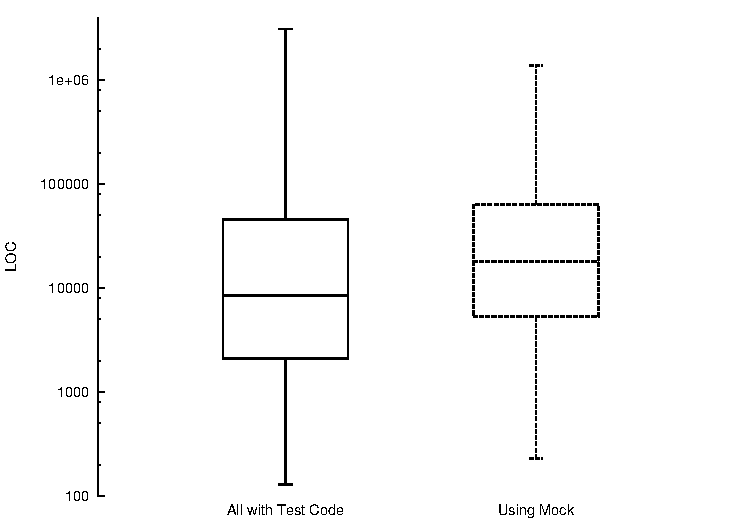
\includegraphics[width=100mm, height=60mm]{mocking/boxplot.pdf}

  \caption{\label{fig:box} Size comparison of software projects using mocking frameworks and all software projects with test code}


\end{figure}

                       
On top of the popularity of mocking frameworks in open source software projects, we are also interested in the market share of various popular mocking frameworks. Therefore, we studied the usage of different mocking frameworks and presented the results in Table~\ref{table:var}. From the table, we can see that, among the four major mocking frameworks, Mockito is the most widely used and is used in more than 70\% of software projects that use mocking frameworks. EasyMock and JMock rank second and third, and are used in about 20\% and 10\% of software projects using frameworks, respectively. JMockit is the least widely used among the four. It should be noted that this observation may not be generalized because it is from 5,000 randomly selected Java projects from GitHub. 

Furthermore, we found that 45 software projects use more than one mocking frameworks. We further studied the projects and found that the main reason for software developers to use multiple mocking frameworks is that, different software testers are more familiar with different mocking frameworks so that they use different mocking frameworks in the testing. Another reason is that the software project is moving from one framework to another. 

\begin{table}
\caption{Popularity of Mocking Frameworks}
\small

\label{table:var}
\centering
\begin{tabular}{|c|r|}
\hline
 Mocking Framework & \# Projects\\
\hline
 Using Mockito & 340\\
 Using EasyMock & 106\\
 Using JMock & 45\\
 Using JMockit & 7\\
 Total & 459\\
 Multiple Mocking Frameworks & 45\\
\hline
\end{tabular}


\end{table}

We observed that mocking frameworks are used widely in software projects. However, the data above just reveals whether a software project involves mocking frameworks in any test class. It is still not known whether mocking frameworks are used in many test classes or only  a small number of test classes. To answer this question, we further studied the number and proportion of test classes that use mocking frameworks and present the results in Table~\ref{table:testclass}

From the table, we can see that, in software projects that use mocking frameworks, on average, 16.8 test classes are using mocking frameworks, accounting for about 29.8\% of all test classes. This observation shows that software testers are not using mock objects for all dependencies. Also, it is not the case that mock objects are used very rare and in only some special cases. 

\begin{table}
\caption{Usage of Mocking Frameworks in Test Classes}
\small

\label{table:testclass}
\centering
\begin{tabular}{|c|r|r|r|r|}
\hline
 & Avg. & Med. & Max. & Min\\
\hline
\# Test Files &16.8&5&1037&1\\
Proportion of Test files &29.8\%&20\%&100\%&0.3\%\\
\hline
\end{tabular}

\end{table}

Moreover, we studied the number of mock objects in one test class and present the results in Table~\ref{table:num}. From the table, we can see that most test classes (77.2\%) have created 3 or less mock objects. Second, we try to understand, for test class that uses mocking frameworks, how many dependency classes are mocked and checked. Specifically, we deem a test class as dependency class if it is imported by the test class. The results are presented in Table~\ref{table:prop}. The table shows that on average about 17\% of dependency classes are mocked by the software testers. Thus, software testers seem to mock only a small portion of all dependency classes of a test class. 

\begin{table}

\caption{Number of Mock Objects in Test Classes}
\small

\label{table:num}
\centering
\begin{tabular}{|c|r|r|}
\hline
\# Mock Objects & \# Test Files & Proportion\\
\hline
1&1270 & 45.3\%\\
2&587 & 21.0\%\\
3&333 & 11.9\%\\
4&210 & 7.5\%\\
5&135 & 4.8\%\\
6&73 & 2.6\%\\
7&49 & 1.7\%\\
8&40 & 1.4\%\\
9&22 & 0.8\%\\
10+&82 & 2.9\%\\
\hline
\end{tabular}

\end{table}


\begin{table}
\caption{Proportion of Mocked Classes}
\small
\label{table:prop}
\centering
\begin{tabular}{|c|r|r|r|r|}
\hline
&Avg. & Med. & Max & Min\\
\hline
\# Mocked Classes &2.7&2&40&1\\
\# Dependency Classes &17.0&14&215&1\\
Proportion of Mocked Clases &17.8\%&14.3\%&100\%&0.9\%\\
\hline
\end{tabular}

\end{table}


\subsection{Usage of Mocking Frameworks}
\label{subsec:usage}


\begin{table}
\caption{Most popular ten APIs in Mockito}
\small
\label{table:mockito}
\centering
\begin{tabular}{|r|r|p{2.6in}|}
\hline
API & Frequency & Description\\
\hline
Mockito.verify&2249 & verify tester's specification of the mock object\\
Mockito.mock&1678 & create an empty mock object\\
Mockito.when&1471 & specify a method in the mock object to be invoked\\
Mockito.spy&403      & partially mock an existing class\\
Mockito.times&232   & specify how many times a method is invoked\\
Mockito.given&161   & Alias of ``when'' for behavior driven development style\\
Mockito.never&152  & specify that a method is never invoked\\
Mockito.verifyNoMoreInteractions & 98 & specify that there are no more interactions between the component under testing and the mock object\\ 
Mockito.doReturn & 85 & specify the return value of a method invocation\\
Mockito.verifyZeroInteractions & 74 & specify that there are no interactions between the component under testing and the mock object\\ 
\hline
\end{tabular}

\end{table}



To answer the second research question, we try to study what APIs in mocking frameworks are most widely used. Since different mocking frameworks have different API sets, in this phase, we study only Mockito and EasyMock, which are the most and second most widely used mocking frameworks. The results are presented in Table~\ref{table:mockito} and Table~\ref{table:easymock}


From Table~\ref{table:mockito} and Table~\ref{table:easymock}, we have the following two main observations. First of all, verification of mock objects are extensively used. This fact shows that software testers do not use mocking frameworks simply as a convenient tool for generating normal test stubs or fake objects, but are using the core features of mock objects (i.e., specifying and verifying interactions between the component under test and the software dependency). Second, several advanced APIs in Mockito are widely used. Such APIs include ``spy'' which partially mock an existing class (i.e., use the mock object for specified method invocations, but the real dependency for other method invocations), ``times'' that specify how many times a certain method is invoked, etc. 

\begin{table}
\caption{Most popular ten APIs in EasyMock}
\small
\label{table:easymock}
\centering
\begin{tabular}{|r|r|p{3in}|}
\hline
API & frequency & description\\
\hline
EasyMock.expect&671& specify a method in the mock object to be invoked\\
EasyMock.createmock&647 & create an empty mock object\\
EasyMock.replay&638 & notice the mock object that the testing of component under testing starts\\
EasyMock.verify&510&verify tester's specification of the mock object\\
EasyMock.expectLastCall&144 &alias for ``expect'' for void methods\\
EasyMock.eq & 90 & expect an value that is equals with a given value\\
EasyMock.createNiceMock & 67 &create a mock object that check the order of method invocations\\
EasyMock.anyObject & 64 & match with any type of arguments when specifying the invocation of a method\\
EasyMock.reportMatcher & 58 & specify a matcher of arguments for specification of method invocations\\
EasyMock.capture & 53 & capture a matched value for later access\\
\hline
\end{tabular}

\end{table}

\subsection{Mocked Dependencies}
\label{subsec:mock}


To answer the third research question, we studied the classes that are mocked by software testers using mocking frameworks. Specifically, we try to find out whether software testers tend to mock library classes and what are the mostly mocked library classes. To find the answer, we check whether the mocked classes are library classes (i.e., classes that are not in the source code base of the software project), and present the results in Table~\ref{table:lib}.The results show that about 39\% of all mocked classes are library classes, so software testers actually tend to mock more classes in the source code, compared with library classes. This shows that the major reason for software testers to perform mocking may be parallel development, instead of accelerating testing process and verifying interactions of classes with dependencies. 


\begin{table}
\caption{Mocking of Library Classes}
\small
\label{table:lib}
\centering
\begin{tabular}{|c|r|r|r|r|}
\hline
&Avg. & Med. & Max & Min\\
\hline
\# Mocked Library Classes &0.85&0.0&18&0\\
Proportion of Library Classes &39.4\%&0\%&100\%&0\%\\
\hline
\end{tabular}

\end{table}

In Table~\ref{table:mostlib}, we present the top 10 mostly mocked library classes. Specifically, the frequencies are the times that the specific class is mocked in all the studied open source software projects. From the table, we can observe that the two major source of mostly mocked classes are the package ``javax.servlet'', and the package ``javax.jcr''. Specifically, the former package is about HTTP request and responses, and the latter package is about the operation of Java Content Repositories. 

\begin{table}
\caption{Mostly Mocked Library Classes}
\small
\label{table:mostlib}
\centering
\begin{tabular}{|r|r|}
\hline
Mocked Library Class& Frequency \\
\hline
javax.servlet.http.HttpServletRequest&44\\
org.fest.assertions.description.Description&41\\
javax.servlet.ServletContext&33\\
javax.jcr.Node&32\\
rx.Observer&24\\
org.openqa.selenium.WebDriver&23\\
javax.servlet.http.HttpServletResponse&22\\
javax.jcr.Property&20\\
javax.jcr.Session&20\\
java.io.InputStream&17\\
\hline
\end{tabular}

\end{table}


\subsection{Summary}
\label{subsec:summary}


To sum up, the major findings of our empirical study are as below.
\begin{itemize}
\item Mocking frameworks and mock objects are used widely among open source Java software projects. However, software testers usually mock only a small number and portion of software dependencies.

\item Verification is widely used to check the specified interaction between the component under testing and the mocked object. Special APIs in both Mockito and EasyMock are widely used, which implies an incompleteness of features for a single mocking framework. 

\item Software testers tend to mock source code classes than libraries, while library classes also take a substantial proportion (40\%) in all mocked classes. The mostly mocked library classes are classes from packages handling HTTP requests / responses, and content repositories. 

\end{itemize}


\subsection{Threats to Validity}
\label{subsec:threat}


The major threat to the internal validity of our study is the potential errors in the programs analyzing the collected software projects and performing statistics. To reduce the threat, we tried our best to write the code carefully to avoid any bugs in the programs. The major threat to the external validity of our study is that our observations may be specific to the subject software projects, and cannot be generalized other software projects. To reduce this threat, we use a large number of subject software projects, and choose the subjects randomly. Also, it is possible that our findings are specific to Java software projects. To further reduce this threat, we plan to carry out similar empirical studies on subjects written with other major programming languages in the future. 






	\vspace{-0.2cm}
\section{Related Work}
\label{sec:related}
	\vspace{-0.1cm}
	
\textbf{Performance Testing and Faults.} Previous work focuses on generating performance test infrastructures and test cases, such as automated performance benchmarking~\cite{KALIBERA}, model-based performance testing framework for workloads~\cite{BARNA11}, using genetic algorithms to expose performance regressions~\cite{LUO16}, learning-based performance testing~\cite{GRECHANIK12}, symbolic-execution-based load-test generation~\cite{ZHANG11}, probabilistic symbolic execution~\cite{Chen2016}, and profiling-based test generation to reach performance bottlenecks~\cite{luoinput2016}. Pradel et al.~\cite{PradelISSTA2014} propose  an approach to support generation of multi-threaded tests based on single-threaded tests. Kwon et al.~\cite{ATC2013} propose an approach to predict execution time of a given input for Android apps. Bound analyses~\cite{SPEED} try to statically estimate the upper bound of loop iterations regarding input sizes, but they cannot be directly applied as the size of collection variables under a  certain test can be difficult to determine. Most recently, Padhye and Sen~\cite{PadhyeICSE2017} propose an  approach to identify collection traversals in program code; such approach has the potential to be used for execution-time prediction. In contrast to such previous work, our approach focuses on prioritizing existing performance test cases. The most related work in this direction is done by Huang et al.~\cite{huang2014performance}, whose differences with our approach are elaborated in Section~\ref{sec:intro}. 

Another related area is research on performance faults, including studies on performance faults~\cite{JIN12, PerfBugStudy}, static performance-fault detection \cite{Nistor14, JOVIC11, KILLIAN10, YAN12}, debugging of known performance faults \cite{SHEN05,HAN12,LEUNG07,AGUILERA03}, automatic patches of performance faults \cite{Nistor15}, and analysis of performance-testing results~\cite{FOO11,FOO10}. 


%The default approach for regression testing is to retest all test cases after releasing a new version, which is an expensive proposition. To solve this problem, there are good collection of industry case studies and research effort on performance regression testing in software systems. 

\noindent\textbf{Test Prioritization and Impact Analysis.} Test prioritization is a well explored area in regression testing to reduce test cost~\cite{HARROLD93,BLACK04,ZHONG06} or to detect functional faults earlier~\cite{ELBAUM00,KIM02,LI07}. Mocking~\cite{MockStudy} is another approach to reduce test cost, but it does not work for performance testing as mocked methods do not have normal execution time. Another related area is test selection or reduction~\cite{ROTHERMEL97,CHEN94,Hao2009} which sets a threshold or other criteria to select/remove part of the test cases. Most of the proposed efforts are based on some coverage criterion for test cases, and/or impact analysis of code commits. The impact analysis falls into three categories: static change impact analysis~\cite{TURVERref,Arnoldref96,Wang2010ASE}, dynamic impact analysis
~\cite{LAW03,ORSO11,APIWATTANAPON05}, and version-history-based impact analysis~\cite{ZIMMERMANN04,SHERRIFF08,MengHima}. Our approach leverages a similar strategy to rank performance tests according to the change impact on them. However, we propose specific techniques to estimate performance impacts, such as collection-loop correlation and performance impact analysis. 

%Functional regression testing is a well explored area to reduce testing cost by test case selection based on test case property andcode modification(), test suite reduction by removing redundancy in test suite () and test cases prioritization orders test case execution in a way to hope (). Different from these work, our goal is to reduce performance regression testing overhead via test suite prioritization based on change impact analysis whether an operation is expensive or lies in hot path. 

%\noindent\textbf{Impact Analysis.} The evolution of software systems and ongoing changes demand for explicit means to assess the impact of a change on existing artifacts and concepts. Thus, software change impact analysis is in the focus of researchers in software engineering. The important difference is that Our proposed method focus on the performance test suite prioritization  via performance impact implication of change.



\section{Conclusion}
\label{sec:conclude}
In this paper, we direct a large scale empirical study on the usage of mocking frameworks in software testing. To perform the study, we collected 6,000 Java software projects from Github, and analyze the source code of the projects to answer a number of questions about the popularity of mocking frameworks, the usage of mocking frameworks, and the mocked classes. 
Our major findings include that mocking frameworks are widely used in practice, and a small portion of dependencies are mocked. This finding shows the requirement of more research on mocking frameworks, as well as on the reasons why developers choose to mock a class while not to mock the other. Furthermore, we find that a number of unique features in Mockito and EasyMock are widely used. This implies that it is possible to build better mocking frameworks by incorporating the most popular features of existing mocking frameworks. We also find that software developers tend to do more mocks on source code classes than library classes, which is not as we expected. 

In the future, we plan to extend our work in the following directions. First of all, we plan to direct similar studies on software projects written in programming languages other than Java to check whether our findings can be generalized. Second, we plan to develop techniques to help software developers and testers make decisions on whether or not a class should be mocked. Third, we plan to develop techniques to generate mock objects automatically with mocking frameworks in automatic unit testing. 


\chapter{An Empirical Study on the Usage of Mocking Frameworks in Software Testing}

\section{Introduction}
\label{sec:intro}
During software evolution, frequent code changes, often including problematic changes, may degrade software performance. For example, a study~\cite{huang2014performance} found that upgrading from MySQL 4.1 to 5.0 caused the loading time of the same web page to increase from 1 second to 20 seconds in a production e-commerce website. Even small performance degradation may result in severe consequence. For example, Google could lose 20\% traffic due to an increase of 500ms latency~\cite{Google}. Amazon could have 1\% decrease in sales due to a 100ms delay in page rendering~\cite{Stevefamov}. \\

Developers can apply systematic, continuous performance regression testing to reveal such performance regressions in early stages~\cite{foxref,poliniref,TSEPerform,MITCHELL,KALIBERA}. But due to its high overhead, performance regression testing is expensive to conduct frequently. Actually, the typical execution cost of popular performance benchmarks varies from tens of minutes to tens of hours~\cite{huang2014performance}, so it is impractical to run all performance test cases for each code commit. Recently, PerfScope~\cite{huang2014performance} was proposed to predict whether a code commit may significantly affect software performance and thus require performance testing. Specifically, PerfScope extracts various features from the original version and the code commit, and trains a classification model for prediction. Although PerfScope helps reduce code commits for performance regression testing, its empirical evaluation shows that a non-trivial proportion of code commits still require performance testing; thus, there is still a strong need of reducing the cost of conducting performance regression testing on a code commit, even after applying PerfScope in practice.\\

%Such problematic changes are referred to as performance regressions in this paper. and GCC from 4.3 to 4.5, Mozilla developers experienced an up to 19\% performance regression, which forced them to consider a complete switchover.Performance regression testing is a major approach to detecting performance regressions, This is widely advocated in academia, open source community and industry .for web servers is 3 minute to 1 hr, for databases is 10 minutes to 3 hrs, for compilers is 1 hr to 20 hrs and for operating systems is 2 hrs to 24 hrs . With the high revision frequency and high testing cost, 


%
%it does not consider the performance impact of code commits on individual test cases, and thus results in two limitations. First,
%

To address such strong need, developers shall prioritize performance test cases on a code commit for three main reasons. First, there can be high cost to execute all performance test cases on a code commit for large systems in practice. Second, as reported in a previous industrial study~\cite{TSEPerform} and our study in Section~\ref{sec:motivation}, various random factors may affect the observed execution time, so it typically requires a large number of repetitive executions to confirm a performance regression. Therefore, with prioritized test cases, developers can better distribute testing resources  (i.e., do more executions on test cases likely to trigger performance regressions). 
Third, a code commit may accelerate some test cases while slowing down others. It is often important for the developers to understand the performance of their software under different scenarios, while a coarse-grained commit-level technique is not helpful on this requirement. \\



%research effort by addressed this problem with PerfScope, or regressional performance testing. Specifically, for each new code commit, PerfScope applied to the code change various program analysis (e.g., hot path analysis, bound analysis, and data dependency analysis) to  to 

%For example, our study shows that it averagely requires 150 executions to confirm a 10\% performance difference, which is typically considered significant, and dynamic techniques bringing in more than 10\% overhead are typically not considered for deployment-time usage~\cite{}. 


%Mozilla’s Talos performance regression detection system~\cite{firefoxTalos} runs performance tests every time a change is pushed to the Firefox source repository~\cite{firefoxperf}. In our empirical evaluation, we observe that one code commit may affect more than 100 test cases. 


 


%There is a useful work on the performance risk implication of code change. But their approach may not accurately assess the risk of performance regression issues because of generic nature of static modeling and lacking profiling information. Furthermore, prioritizing commits is not enough to address performance regression because  a code changes touches several test cases is very common during the evolution of software. In our study, we found that some commits touches more than 100 test cases. So the key difference is that we focus  on the prioritizing test cases in regressional performance testing via performance impact analysis of code changes that includes one time profiling and static modeling.

To develop an effective test-prioritization solution for performance regression testing, we focus on \textit{collection-intensive software}, an important type of modern software whose execution time is heavily spent on loading, manipulating, and writing collections of data. Collections are widely used in software for scalable data storage and processing, and thus collection-intensive software is very common. Examples include libraries for data structures, text formating and parsing, mathematics, image processing, etc. Also, collection-intensive software is often used as components in complex systems. Moreover, a recent study~\cite{JIN12} shows that a large portion of performance bugs are related to loops, which are often used to iterate through collections. Our statistics show that 89\% and 77\% of loops iterate through collections for our two subjects Xalan and Apache Commons Math, respectively.\\

%improper iteration on collections has been identified as one of the most
%

For collection-intensive software, a straightforward approach to prioritizing performance test cases on a code commit would be measuring collection iterations (e.g., loops) impacted by the code commit and executed by each test case. However, such an approach may not be precise enough to differentiate test cases in the presence of newly added iterations, manipulations, and processing of collections, as well as their effect on existing collection iterations. Consider the simplified code example from Xalan in Listing~\ref{list:example-p3}. The code commit involves a new loop, and its location may or may not be at the hot spot for all or most test cases. Therefore, its impact on different test cases may largely depend on the different iteration counts of the added loop, the side effect of changing variable \CodeIn{list}, and the operations in the loop. Since Loop$_B$ depends on a collection variable \CodeIn{limits}, which further depends on Loop$_A$, we can infer the test-case-specific iteration count of Loop$_B$ from that of Loop$_A$; such iteration count can be acquired by profiling the base version for all test cases. Furthermore, we can infer the effect of adding \CodeIn{list.add(...)} on \CodeIn{list} with the iteration count of Loop$_B$, and update the iteration count of loops dependent on \CodeIn{list}. Moreover, we can enhance the estimation precision by using test-case-specific execution time of operations (e.g., \CodeIn{new Arc(...)}). 


{\fontsize{10}{10}
	\begin{lstlisting}[columns=flexible,language=Java,caption=Collection Loop Correlation, label={list:example-p3}]
	  while(i <= m\_size){ //Loop A
	    limits.add(new Limit(...))
	    ...
	  }
	  ...
	+ Collections.sort(limits);
	+ for (int i = 0; i < limits.size()-1; i++) { //Loop B
	+   list.add(new Arc(limits.get(i), ...));
	+ }
	\end{lstlisting}
}


These observations inspire us for three main insights to effectively model a code commit and its effect on existing collections and their iterations. First, collection sizes (e.g., \CodeIn{limits.size()}) and loop-iteration counts (e.g., Loop$_B$) can often be correlated, so collection sizes can be inferred from loop-iteration numbers and vice versa. Also, collection variables (e.g., \CodeIn{limits}) can be used as bridges to infer iteration counts of new loops (e.g., Loop$_B$) from existing loops (e.g., Loop$_A$). Second, collection manipulations (e.g., \CodeIn{list.add(...)}) are often inside loops, so the size of collections referred by collection variables (e.g. \CodeIn{list}) can be estimated from loop-iteration counts (e.g., Loop$_B$). Third, due to the large number of elements in collections, the average processing time of elements (e.g., \CodeIn{new Arc(...)}) is relatively stable, so a method's average execution time in the new version may be estimated from that in the base version.\\ 

Based on the three insights, we propose PerfRanker, which consists of four automatic steps. First, on a base version, we execute each test case in a profiling mode to collect information about the test execution, including the runtime call graph and the iteration counts of all executed loops. We also perform static analysis to capture the dependency among collection objects and loops. Second, based on the profiling information, we construct a performance model for each test case. Third, given a code commit, we estimate the execution time of each test case on the new version (formed by the code commit) by extending and revising its old performance model. We use profiling information and loop-collection correlations to infer parameters of the new performance model, and refer to this step as \textit{Performance Impact Analysis}. Fourth, we rank all the test cases based on the performance impact on them.\\

%its impact on each test case from two aspects: the execution time of the added and removed code in the revised method, and the execution time of the loops affected by the collection objects which are return values of revised methods. 




%To address the two limitations above, we propose a novel approach to prioritize individual test cases in performance regression testing via performance impact analysis, which estimates the impact of a given code revision on the execution time of a given test case. 



%our algorithm automatically takes the information in each code commit by statically analyzing the added code and removed code from automatically generated diff of each commit. Incorporating the profile and static information into each test case's call graph we determine the run-time cost and the execution frequency of the code affected by code changes. 

We implement our approach and apply it on two sets of code commits collected from popular open source collection-intensive projects: Apache Commons Math and Xalan. To measure the effectiveness of test case prioritization for a code commit in performance regression testing, we use three metrics: (1) \textit{APFD-P} (Average Percentage Fault Detected for Performance), an adapted version of the APFD metric~\cite{AlexeyAPFD} for performance testing, (2) \textit{DCG}~\cite{NDCG}, a general metric for comparing the similarity of two sequences, and (3) \textit{Top-N Percentile}, which calculates the percentage of test cases needed to be executed to cover the top N test cases whose execution time is most affected by the code commit. Our evaluation results show that, compared with the best of the three other baseline approaches, our approach achieves an average improvement of 17.6 percentage points on \textit{APFD-P} and 27.4 percentage points on DCG. Furthermore, for Apache Commons Math and Xalan, our approach is able to rank top 1 affected test case within top 8\% and top 16\% test cases, and top 3 affected test cases within top 37\% and 30\% test cases, respectively. 

%Since we are not aware of previous research efforts on prioritizing test cases for performance regression testing, we developed  for Apache Commons Math, and an improvement of 16.6 percentage points on APFD and 27.2 percentage points on DCG for Xalan, respectively

%calculated impact score is used with adaptive APFD and DCG metric formula to rank the test case which shows that they can significantly reduce the cost of performance regression. 


This paper makes the following major contributions:
  \vspace{-0.1cm}
\begin{itemize}
  \item A novel approach to prioritizing test cases in performance regression testing of collection-intensive software.
  
  
%supported by a novel technique called performance impact analysis which estimates the performance impact of code revisions on test cases.
  
%  \item A motivation study on the number of executions required to acquire stable performance testing results.
    
    
  \item Adaptation of the APFD metric to measure the result of test prioritization for performance regression testing. 
    
  \item An evaluation of our approach on real-world code commits from two popular open source collection-intensive projects. 
  
\end{itemize}
  
  
%The rest parts of this paper are organized as follows. In Section~\ref{sec:motivation}, we present a motivation study showing that multiple test executions are required to confirm a performance regression. In Section~\ref{sec:approach}, we introduce our approach and performance impact analysis in details. We present our evaluation results in Section~\ref{sec:evaluation}, and discuss some related issues in Section~\ref{sec:discuss}. Before we conclude in Section~\ref{sec:conclusion}, we introduce related research efforts in Section~\ref{sec:related}, and indicate some future work in Section~\ref{sec:future}.

\section{Background}
\label{sec:backgroundmock}
In this section, we first introduce some basic background knowledge on mocking objects. Then, we introduce the mechanism of mocking frameworks and some major mocking frameworks.
\subsection{Mocking Objects}

Mocking objects are used in software testing to simulate software dependencies so that the testing process can be accelerated and the testing scope can be limited to the component under test (instead of going beyond the interface of dependencies and invoke potential bugs relevant to dependencies). To simulate real dependencies, mock objects typically have the same interface as the objects they mimic. Therefore, the client object remains unaware of whether it is using a real object or a mock object. 

%The major difference between mock object and other test doubles (i.e., objects simulating software dependencies, such as test stubs, fake objects) is that, on top of simulating software dependencies, mock objects also contain assertions of their own. Mock objects will examine the context of each invocation of their methods, on whether a method is invoked, whether several methods are invoked in correct order, and whether arguments of the methods are passed in correctly. 

For example, when testing an email client, software testers may not use the real email server which has slow response and random failures. By contrast, they may construct a fake email server object (a mock object) that returns whatever expected by the software testers. The expected return value can be either a simple success code for the testing of normal functioning of the email client, or a server error code for the testing of error handling of the email client. Such a fake email server helps to reduce testing time as well as to explore the handling of server errors that are very hard to invoke with a real server. However, when such a simplified email server is used, it is hard for testers to tell whether the email client has invoked the email server in a correct order (if multiple-step configuration of the server is required), or whether the client has passed correct arguments to the server. 

Therefore, the software testers may further have some code in the fake email server to check whether the client interacts with it correctly and passes correct arguments. With such a mock email server, software testers can perform quick and controllable testing of the email client without losing the thorough exploration of the interface between the email client and the email server.


\subsection{Mocking Frameworks}

As mentioned in the previous section, mocking objects are desirable for simulating software dependencies in software testing. However, since mock objects need to perform various checking of the invocations, it is usually nontrivial to write such mock objects, and thus the benefit of using mock objects can be undermined by the effort spent on writing mock objects. 

To solve this problem, in the past decade, people have developed various mocking frameworks to generate mock objects automatically. A code sample of using a mocking framework is presented below. With a mocking framework, software testers first create an empty mock object (Line 3). Then, for the created mock object, software testers can specify a number of invocation for the object to check, both on the order of the invocations and the correctness of the arguments (Line 6). After that, in the test code, testers run the component under test as usual but with created mock objects (Line 8). During the execution, if the specified invocation order or arguments are not satisfied, the mock object will throw a test failure so that the software testers know that something wrong happened (Line 9). \\


\begin{lstlisting}[language=Java]
1: @Test
2: public void testEmailClient(){
3:     Server sv = EasyMock.
            CreateMock(Server.class); 
4:     Client c = new Client(sv);         
5:     Email em = new Email(...)
        //record
6:     EasyMock.expect(sv.send(em)).
            andReturn(0);
        //replay
7:     EasyMock.replay(sv);
8:     c.send(em)
9:     EasyMock.verify(sv)
10:}
\end{lstlisting}


For each major programming language, there have been a number of mocking frameworks developed, such as Mockito, EasyMock, and JMock for Java, pmock, mox for Python, and NMock, Moq for C\#. All of these mocking frameworks support the basic features of mocking including the creation of mock objects, the specification of invocation orders and arguments, and the verification of the specifications. The differences between these mocking frameworks are mainly on the design of APIs and supporting of advanced specifications such as checking the number of invocations of a certain method. 


\section{Design}
\label{sec:design}
In this section, we introduce the design of our empirical study on the usage of mocking frameworks among developers of open source software projects. 
\vspace{-0.2cm}

\subsection{Research Questions}
\label{subsec:rq}
\vspace{-0.2cm}

In this study, we design an experiment to answer the following research questions. By answering these questions, we try to understand whether and how software developers and testers use mocking frameworks to handle dependencies in the testing of open source software projects. 
\begin{itemize}
\item \textbf{RQ1:} How popular are mocking frameworks that are used in the testing of open source Java software projects? Are developers trying to mock most or all of dependencies?
\item \textbf{RQ2:} What features of mocking frameworks are most frequently used in the testing of open source software projects?
\item \textbf{RQ3:} What types of dependencies developers tend to mock?
\end{itemize}
\vspace{-0.2cm}

\subsection{Subjects}
\vspace{-0.2cm}

To perform our empirical study, we randomly downloaded 5,000 Java software projects from Github. We choose to focus on Java software projects because Java is one of the most widely used object-oriented programming language, and due to the popularity of Java in the open source community, a large number of open source Java software projects may serve as subjects. When selecting subject projects, we first search Java projects in Github with 26 keywords from 'a' to 'z', and then, we randomly sample 5000 projects from the merged search results. For each project, we consider only the most recent version. 

The basic information of the 5,000 Java software projects are presented in Table~\ref{table:basic}.

\begin{table}
\caption{Basic Information of Subjects Used in Study}
\label{table:basic}
\centering
\begin{tabular}{|c|r|r|r|r|}
\hline
Info Type & Avg. & Med. & Max. & Min\\
\hline
\# Java Files &153&18&10,141&1\\
LOC  &25,305&1,833&3,094,265&0\\
\# Test Files  &16.4&0&3,335&0\\
\# Developers  &3.0&1&39&1\\
\# Versions  &11.4&1&1694&1\\
\hline
\end{tabular}
\end{table}

In Table~\ref{table:basic}, we present five types of basic information of the collected software projects, which are in the Lines 2-6 of the table. Specifically, Line 2 presents the number of Java Files in the project. It should be noted that some of the software projects may be developed in multiple programming languages and may involve other types of source code files. In our study, we focus only on the Java part of such software projects. Line 3 presents the total lines of source code in the Java source files. Line 4 presents the number of test files in the software projects. Specifically, we consider a Java source file as a test file if it uses any library classes from JUnit or TestNG, which are the two major test frameworks for Java and the only test frameworks we notice the collected software projects are using. It should be noted that, in some software projects, a test class $C$ may extend a library class in test frameworks, and other test files use only $C$ but not any library classes in test frameworks. So in our study, we also consider the test files that indirectly use library classes in test frameworks by using classes like $C$. Line 5 and Line 6 present the number of developers and the number of versions (i.e. code commits) of the software projects. 

Due to the large number of subjects, we are not able to present the basic information of individual software projects. Instead, we present the statistical information of the software projects. Column 2-5 present the average, medium, maximum and minimum of all types of information, respectively.  

From Table~\ref{table:basic}, we can see that the chosen subjects vary largely in their sizes, testing efforts, number of developers, and history. The average size of the subjects are 25KLOC, and the largest subject has more than 3 million lines of code. Furthermore, more than half of the subjects have no test code (the medium of number of test files is 0), and the average number of test classes is 16.4. 
\vspace{-0.2cm}

\subsection{Process}
\vspace{-0.2cm}

To answer the research questions listed in Section~\ref{subsec:rq}, for each of the collected subject, we first identify all the Java source files and test files. Then, we parse these files to extract the code relevant to mocking frameworks. 

In particular, we consider the four most popular Java mocking frameworks in our study: Mockito, EasyMock, JMock, and JMockit. PowerMock is another popular mocking framework, but it is actually an extension of Mockito and EasyMock frameworks, and typically software projects using PowerMock will use at least one of Mockito or EasyMock frameworks, so we do not consider PowerMock in our study. 

The four investigated frameworks have some specific characteristics. EasyMock
requires developers to specify the type of the mock object at the creation point (i.e., whether the mock object is strict or not, and whether to raise exceptions when there are unexpected methods invoked). Typically, EasyMock is more strict to raise more run time errors, and the interface is not very easy to learn (comments from StackOverflow). Mockito actually origins from EasyMock, and it
provides a very simple API interface to create mocking objects (not strict by default) and support annotations to specify the classes to be mocked. Mockito also provides very good spy features that verifies the dependency-related interaction of the class under testing on the real dependency classes. JMock is similar to EasyMock in most aspects. JMockit uses class-map as its underlying technique for mocking and thus can mock final classes. 


From the relevant code, we extract the information that can help answer our research questions, Specifically, we extract a data set of API signatures of each mocking framework from their API documents, and developed a AST-tree-based code analyzer analyze the source code of subject projects extract all relevant API invocations. Based on these API invocations, we are able to identify the API method in mocking frameworks used, the dependency classes being mocked, etc. 


\section{Empirical Study Results}
\label{sec:studymock}


In this section, we present the details and results of our empirical study. Specifically, we present the study to answer the research questions 1 to 3 in Section~\ref{subsec:pop}, Section~\ref{subsec:usage}, and Section~\ref{subsec:mock}, respectively. We summarize our findings in Section~\ref{subsec:summary}, and present the threats to validity in Section~\ref{subsec:threat}. 

\subsection{Popularity of Mocking Frameworks}
\label{subsec:pop}


To answer the first research question, we study the number of software projects using mocking frameworks among the 5,000 downloaded software projects. Specifically, among the 5,000 software projects, 2,046 has at least one test class (a class importing and use any class from JUnit or TestNg). Among the 2,046 projects, 459 projects (23\%) uses at least one mocking framework. We guess that developers of large software projects tend to use mocking frameworks, so we compare the size distribution of software projects using mocking frameworks with the size distribution of all software projects having test code, and present the results in Figure~\ref{fig:box}. The figure shows that the size of software projects using mocking frameworks tends to be larger than other software projects with test code. Specifically, the median size of software projects using mocking frameworks is 16KLOC,  compared to 8.4KLOC of all software projects with test code (software projects in the latter set include software projects in the former set). At the same time, we also found that there are many large software projects do not use any of the investigated mocking frameworks. Furthermore, among the software projects (with test code) that are larger than 10KLOC, and 100KLOC, the proportion of software projects using mocking frameworks goes up to 30\% and 34\%, respectively. 

\begin{figure}


  \center
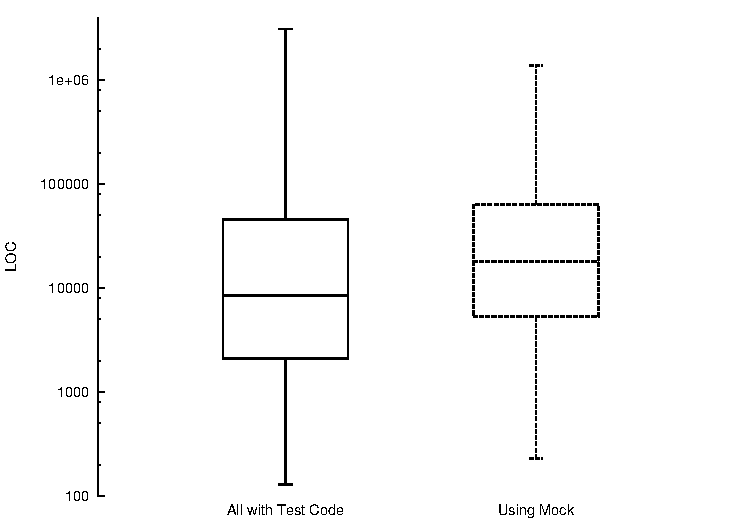
\includegraphics[width=100mm, height=60mm]{mocking/boxplot.pdf}

  \caption{\label{fig:box} Size comparison of software projects using mocking frameworks and all software projects with test code}


\end{figure}

                       
On top of the popularity of mocking frameworks in open source software projects, we are also interested in the market share of various popular mocking frameworks. Therefore, we studied the usage of different mocking frameworks and presented the results in Table~\ref{table:var}. From the table, we can see that, among the four major mocking frameworks, Mockito is the most widely used and is used in more than 70\% of software projects that use mocking frameworks. EasyMock and JMock rank second and third, and are used in about 20\% and 10\% of software projects using frameworks, respectively. JMockit is the least widely used among the four. It should be noted that this observation may not be generalized because it is from 5,000 randomly selected Java projects from GitHub. 

Furthermore, we found that 45 software projects use more than one mocking frameworks. We further studied the projects and found that the main reason for software developers to use multiple mocking frameworks is that, different software testers are more familiar with different mocking frameworks so that they use different mocking frameworks in the testing. Another reason is that the software project is moving from one framework to another. 

\begin{table}
\caption{Popularity of Mocking Frameworks}
\small

\label{table:var}
\centering
\begin{tabular}{|c|r|}
\hline
 Mocking Framework & \# Projects\\
\hline
 Using Mockito & 340\\
 Using EasyMock & 106\\
 Using JMock & 45\\
 Using JMockit & 7\\
 Total & 459\\
 Multiple Mocking Frameworks & 45\\
\hline
\end{tabular}


\end{table}

We observed that mocking frameworks are used widely in software projects. However, the data above just reveals whether a software project involves mocking frameworks in any test class. It is still not known whether mocking frameworks are used in many test classes or only  a small number of test classes. To answer this question, we further studied the number and proportion of test classes that use mocking frameworks and present the results in Table~\ref{table:testclass}

From the table, we can see that, in software projects that use mocking frameworks, on average, 16.8 test classes are using mocking frameworks, accounting for about 29.8\% of all test classes. This observation shows that software testers are not using mock objects for all dependencies. Also, it is not the case that mock objects are used very rare and in only some special cases. 

\begin{table}
\caption{Usage of Mocking Frameworks in Test Classes}
\small

\label{table:testclass}
\centering
\begin{tabular}{|c|r|r|r|r|}
\hline
 & Avg. & Med. & Max. & Min\\
\hline
\# Test Files &16.8&5&1037&1\\
Proportion of Test files &29.8\%&20\%&100\%&0.3\%\\
\hline
\end{tabular}

\end{table}

Moreover, we studied the number of mock objects in one test class and present the results in Table~\ref{table:num}. From the table, we can see that most test classes (77.2\%) have created 3 or less mock objects. Second, we try to understand, for test class that uses mocking frameworks, how many dependency classes are mocked and checked. Specifically, we deem a test class as dependency class if it is imported by the test class. The results are presented in Table~\ref{table:prop}. The table shows that on average about 17\% of dependency classes are mocked by the software testers. Thus, software testers seem to mock only a small portion of all dependency classes of a test class. 

\begin{table}

\caption{Number of Mock Objects in Test Classes}
\small

\label{table:num}
\centering
\begin{tabular}{|c|r|r|}
\hline
\# Mock Objects & \# Test Files & Proportion\\
\hline
1&1270 & 45.3\%\\
2&587 & 21.0\%\\
3&333 & 11.9\%\\
4&210 & 7.5\%\\
5&135 & 4.8\%\\
6&73 & 2.6\%\\
7&49 & 1.7\%\\
8&40 & 1.4\%\\
9&22 & 0.8\%\\
10+&82 & 2.9\%\\
\hline
\end{tabular}

\end{table}


\begin{table}
\caption{Proportion of Mocked Classes}
\small
\label{table:prop}
\centering
\begin{tabular}{|c|r|r|r|r|}
\hline
&Avg. & Med. & Max & Min\\
\hline
\# Mocked Classes &2.7&2&40&1\\
\# Dependency Classes &17.0&14&215&1\\
Proportion of Mocked Clases &17.8\%&14.3\%&100\%&0.9\%\\
\hline
\end{tabular}

\end{table}


\subsection{Usage of Mocking Frameworks}
\label{subsec:usage}


\begin{table}
\caption{Most popular ten APIs in Mockito}
\small
\label{table:mockito}
\centering
\begin{tabular}{|r|r|p{2.6in}|}
\hline
API & Frequency & Description\\
\hline
Mockito.verify&2249 & verify tester's specification of the mock object\\
Mockito.mock&1678 & create an empty mock object\\
Mockito.when&1471 & specify a method in the mock object to be invoked\\
Mockito.spy&403      & partially mock an existing class\\
Mockito.times&232   & specify how many times a method is invoked\\
Mockito.given&161   & Alias of ``when'' for behavior driven development style\\
Mockito.never&152  & specify that a method is never invoked\\
Mockito.verifyNoMoreInteractions & 98 & specify that there are no more interactions between the component under testing and the mock object\\ 
Mockito.doReturn & 85 & specify the return value of a method invocation\\
Mockito.verifyZeroInteractions & 74 & specify that there are no interactions between the component under testing and the mock object\\ 
\hline
\end{tabular}

\end{table}



To answer the second research question, we try to study what APIs in mocking frameworks are most widely used. Since different mocking frameworks have different API sets, in this phase, we study only Mockito and EasyMock, which are the most and second most widely used mocking frameworks. The results are presented in Table~\ref{table:mockito} and Table~\ref{table:easymock}


From Table~\ref{table:mockito} and Table~\ref{table:easymock}, we have the following two main observations. First of all, verification of mock objects are extensively used. This fact shows that software testers do not use mocking frameworks simply as a convenient tool for generating normal test stubs or fake objects, but are using the core features of mock objects (i.e., specifying and verifying interactions between the component under test and the software dependency). Second, several advanced APIs in Mockito are widely used. Such APIs include ``spy'' which partially mock an existing class (i.e., use the mock object for specified method invocations, but the real dependency for other method invocations), ``times'' that specify how many times a certain method is invoked, etc. 

\begin{table}
\caption{Most popular ten APIs in EasyMock}
\small
\label{table:easymock}
\centering
\begin{tabular}{|r|r|p{3in}|}
\hline
API & frequency & description\\
\hline
EasyMock.expect&671& specify a method in the mock object to be invoked\\
EasyMock.createmock&647 & create an empty mock object\\
EasyMock.replay&638 & notice the mock object that the testing of component under testing starts\\
EasyMock.verify&510&verify tester's specification of the mock object\\
EasyMock.expectLastCall&144 &alias for ``expect'' for void methods\\
EasyMock.eq & 90 & expect an value that is equals with a given value\\
EasyMock.createNiceMock & 67 &create a mock object that check the order of method invocations\\
EasyMock.anyObject & 64 & match with any type of arguments when specifying the invocation of a method\\
EasyMock.reportMatcher & 58 & specify a matcher of arguments for specification of method invocations\\
EasyMock.capture & 53 & capture a matched value for later access\\
\hline
\end{tabular}

\end{table}

\subsection{Mocked Dependencies}
\label{subsec:mock}


To answer the third research question, we studied the classes that are mocked by software testers using mocking frameworks. Specifically, we try to find out whether software testers tend to mock library classes and what are the mostly mocked library classes. To find the answer, we check whether the mocked classes are library classes (i.e., classes that are not in the source code base of the software project), and present the results in Table~\ref{table:lib}.The results show that about 39\% of all mocked classes are library classes, so software testers actually tend to mock more classes in the source code, compared with library classes. This shows that the major reason for software testers to perform mocking may be parallel development, instead of accelerating testing process and verifying interactions of classes with dependencies. 


\begin{table}
\caption{Mocking of Library Classes}
\small
\label{table:lib}
\centering
\begin{tabular}{|c|r|r|r|r|}
\hline
&Avg. & Med. & Max & Min\\
\hline
\# Mocked Library Classes &0.85&0.0&18&0\\
Proportion of Library Classes &39.4\%&0\%&100\%&0\%\\
\hline
\end{tabular}

\end{table}

In Table~\ref{table:mostlib}, we present the top 10 mostly mocked library classes. Specifically, the frequencies are the times that the specific class is mocked in all the studied open source software projects. From the table, we can observe that the two major source of mostly mocked classes are the package ``javax.servlet'', and the package ``javax.jcr''. Specifically, the former package is about HTTP request and responses, and the latter package is about the operation of Java Content Repositories. 

\begin{table}
\caption{Mostly Mocked Library Classes}
\small
\label{table:mostlib}
\centering
\begin{tabular}{|r|r|}
\hline
Mocked Library Class& Frequency \\
\hline
javax.servlet.http.HttpServletRequest&44\\
org.fest.assertions.description.Description&41\\
javax.servlet.ServletContext&33\\
javax.jcr.Node&32\\
rx.Observer&24\\
org.openqa.selenium.WebDriver&23\\
javax.servlet.http.HttpServletResponse&22\\
javax.jcr.Property&20\\
javax.jcr.Session&20\\
java.io.InputStream&17\\
\hline
\end{tabular}

\end{table}


\subsection{Summary}
\label{subsec:summary}


To sum up, the major findings of our empirical study are as below.
\begin{itemize}
\item Mocking frameworks and mock objects are used widely among open source Java software projects. However, software testers usually mock only a small number and portion of software dependencies.

\item Verification is widely used to check the specified interaction between the component under testing and the mocked object. Special APIs in both Mockito and EasyMock are widely used, which implies an incompleteness of features for a single mocking framework. 

\item Software testers tend to mock source code classes than libraries, while library classes also take a substantial proportion (40\%) in all mocked classes. The mostly mocked library classes are classes from packages handling HTTP requests / responses, and content repositories. 

\end{itemize}


\subsection{Threats to Validity}
\label{subsec:threat}


The major threat to the internal validity of our study is the potential errors in the programs analyzing the collected software projects and performing statistics. To reduce the threat, we tried our best to write the code carefully to avoid any bugs in the programs. The major threat to the external validity of our study is that our observations may be specific to the subject software projects, and cannot be generalized other software projects. To reduce this threat, we use a large number of subject software projects, and choose the subjects randomly. Also, it is possible that our findings are specific to Java software projects. To further reduce this threat, we plan to carry out similar empirical studies on subjects written with other major programming languages in the future. 






	\vspace{-0.2cm}
\section{Related Work}
\label{sec:related}
	\vspace{-0.1cm}
	
\textbf{Performance Testing and Faults.} Previous work focuses on generating performance test infrastructures and test cases, such as automated performance benchmarking~\cite{KALIBERA}, model-based performance testing framework for workloads~\cite{BARNA11}, using genetic algorithms to expose performance regressions~\cite{LUO16}, learning-based performance testing~\cite{GRECHANIK12}, symbolic-execution-based load-test generation~\cite{ZHANG11}, probabilistic symbolic execution~\cite{Chen2016}, and profiling-based test generation to reach performance bottlenecks~\cite{luoinput2016}. Pradel et al.~\cite{PradelISSTA2014} propose  an approach to support generation of multi-threaded tests based on single-threaded tests. Kwon et al.~\cite{ATC2013} propose an approach to predict execution time of a given input for Android apps. Bound analyses~\cite{SPEED} try to statically estimate the upper bound of loop iterations regarding input sizes, but they cannot be directly applied as the size of collection variables under a  certain test can be difficult to determine. Most recently, Padhye and Sen~\cite{PadhyeICSE2017} propose an  approach to identify collection traversals in program code; such approach has the potential to be used for execution-time prediction. In contrast to such previous work, our approach focuses on prioritizing existing performance test cases. The most related work in this direction is done by Huang et al.~\cite{huang2014performance}, whose differences with our approach are elaborated in Section~\ref{sec:intro}. 

Another related area is research on performance faults, including studies on performance faults~\cite{JIN12, PerfBugStudy}, static performance-fault detection \cite{Nistor14, JOVIC11, KILLIAN10, YAN12}, debugging of known performance faults \cite{SHEN05,HAN12,LEUNG07,AGUILERA03}, automatic patches of performance faults \cite{Nistor15}, and analysis of performance-testing results~\cite{FOO11,FOO10}. 


%The default approach for regression testing is to retest all test cases after releasing a new version, which is an expensive proposition. To solve this problem, there are good collection of industry case studies and research effort on performance regression testing in software systems. 

\noindent\textbf{Test Prioritization and Impact Analysis.} Test prioritization is a well explored area in regression testing to reduce test cost~\cite{HARROLD93,BLACK04,ZHONG06} or to detect functional faults earlier~\cite{ELBAUM00,KIM02,LI07}. Mocking~\cite{MockStudy} is another approach to reduce test cost, but it does not work for performance testing as mocked methods do not have normal execution time. Another related area is test selection or reduction~\cite{ROTHERMEL97,CHEN94,Hao2009} which sets a threshold or other criteria to select/remove part of the test cases. Most of the proposed efforts are based on some coverage criterion for test cases, and/or impact analysis of code commits. The impact analysis falls into three categories: static change impact analysis~\cite{TURVERref,Arnoldref96,Wang2010ASE}, dynamic impact analysis
~\cite{LAW03,ORSO11,APIWATTANAPON05}, and version-history-based impact analysis~\cite{ZIMMERMANN04,SHERRIFF08,MengHima}. Our approach leverages a similar strategy to rank performance tests according to the change impact on them. However, we propose specific techniques to estimate performance impacts, such as collection-loop correlation and performance impact analysis. 

%Functional regression testing is a well explored area to reduce testing cost by test case selection based on test case property andcode modification(), test suite reduction by removing redundancy in test suite () and test cases prioritization orders test case execution in a way to hope (). Different from these work, our goal is to reduce performance regression testing overhead via test suite prioritization based on change impact analysis whether an operation is expensive or lies in hot path. 

%\noindent\textbf{Impact Analysis.} The evolution of software systems and ongoing changes demand for explicit means to assess the impact of a change on existing artifacts and concepts. Thus, software change impact analysis is in the focus of researchers in software engineering. The important difference is that Our proposed method focus on the performance test suite prioritization  via performance impact implication of change.



\section{Conclusion}
\label{sec:conclude}
In this paper, we direct a large scale empirical study on the usage of mocking frameworks in software testing. To perform the study, we collected 6,000 Java software projects from Github, and analyze the source code of the projects to answer a number of questions about the popularity of mocking frameworks, the usage of mocking frameworks, and the mocked classes. 
Our major findings include that mocking frameworks are widely used in practice, and a small portion of dependencies are mocked. This finding shows the requirement of more research on mocking frameworks, as well as on the reasons why developers choose to mock a class while not to mock the other. Furthermore, we find that a number of unique features in Mockito and EasyMock are widely used. This implies that it is possible to build better mocking frameworks by incorporating the most popular features of existing mocking frameworks. We also find that software developers tend to do more mocks on source code classes than library classes, which is not as we expected. 

In the future, we plan to extend our work in the following directions. First of all, we plan to direct similar studies on software projects written in programming languages other than Java to check whether our findings can be generalized. Second, we plan to develop techniques to help software developers and testers make decisions on whether or not a class should be mocked. Third, we plan to develop techniques to generate mock objects automatically with mocking frameworks in automatic unit testing. 


\chapter{Beyond API Signatures: Behavioral Backward Incompatibilities of Java Software Libraries}

\section{Introduction}
\label{sec:intro}
During software evolution, frequent code changes, often including problematic changes, may degrade software performance. For example, a study~\cite{huang2014performance} found that upgrading from MySQL 4.1 to 5.0 caused the loading time of the same web page to increase from 1 second to 20 seconds in a production e-commerce website. Even small performance degradation may result in severe consequence. For example, Google could lose 20\% traffic due to an increase of 500ms latency~\cite{Google}. Amazon could have 1\% decrease in sales due to a 100ms delay in page rendering~\cite{Stevefamov}. \\

Developers can apply systematic, continuous performance regression testing to reveal such performance regressions in early stages~\cite{foxref,poliniref,TSEPerform,MITCHELL,KALIBERA}. But due to its high overhead, performance regression testing is expensive to conduct frequently. Actually, the typical execution cost of popular performance benchmarks varies from tens of minutes to tens of hours~\cite{huang2014performance}, so it is impractical to run all performance test cases for each code commit. Recently, PerfScope~\cite{huang2014performance} was proposed to predict whether a code commit may significantly affect software performance and thus require performance testing. Specifically, PerfScope extracts various features from the original version and the code commit, and trains a classification model for prediction. Although PerfScope helps reduce code commits for performance regression testing, its empirical evaluation shows that a non-trivial proportion of code commits still require performance testing; thus, there is still a strong need of reducing the cost of conducting performance regression testing on a code commit, even after applying PerfScope in practice.\\

%Such problematic changes are referred to as performance regressions in this paper. and GCC from 4.3 to 4.5, Mozilla developers experienced an up to 19\% performance regression, which forced them to consider a complete switchover.Performance regression testing is a major approach to detecting performance regressions, This is widely advocated in academia, open source community and industry .for web servers is 3 minute to 1 hr, for databases is 10 minutes to 3 hrs, for compilers is 1 hr to 20 hrs and for operating systems is 2 hrs to 24 hrs . With the high revision frequency and high testing cost, 


%
%it does not consider the performance impact of code commits on individual test cases, and thus results in two limitations. First,
%

To address such strong need, developers shall prioritize performance test cases on a code commit for three main reasons. First, there can be high cost to execute all performance test cases on a code commit for large systems in practice. Second, as reported in a previous industrial study~\cite{TSEPerform} and our study in Section~\ref{sec:motivation}, various random factors may affect the observed execution time, so it typically requires a large number of repetitive executions to confirm a performance regression. Therefore, with prioritized test cases, developers can better distribute testing resources  (i.e., do more executions on test cases likely to trigger performance regressions). 
Third, a code commit may accelerate some test cases while slowing down others. It is often important for the developers to understand the performance of their software under different scenarios, while a coarse-grained commit-level technique is not helpful on this requirement. \\



%research effort by addressed this problem with PerfScope, or regressional performance testing. Specifically, for each new code commit, PerfScope applied to the code change various program analysis (e.g., hot path analysis, bound analysis, and data dependency analysis) to  to 

%For example, our study shows that it averagely requires 150 executions to confirm a 10\% performance difference, which is typically considered significant, and dynamic techniques bringing in more than 10\% overhead are typically not considered for deployment-time usage~\cite{}. 


%Mozilla’s Talos performance regression detection system~\cite{firefoxTalos} runs performance tests every time a change is pushed to the Firefox source repository~\cite{firefoxperf}. In our empirical evaluation, we observe that one code commit may affect more than 100 test cases. 


 


%There is a useful work on the performance risk implication of code change. But their approach may not accurately assess the risk of performance regression issues because of generic nature of static modeling and lacking profiling information. Furthermore, prioritizing commits is not enough to address performance regression because  a code changes touches several test cases is very common during the evolution of software. In our study, we found that some commits touches more than 100 test cases. So the key difference is that we focus  on the prioritizing test cases in regressional performance testing via performance impact analysis of code changes that includes one time profiling and static modeling.

To develop an effective test-prioritization solution for performance regression testing, we focus on \textit{collection-intensive software}, an important type of modern software whose execution time is heavily spent on loading, manipulating, and writing collections of data. Collections are widely used in software for scalable data storage and processing, and thus collection-intensive software is very common. Examples include libraries for data structures, text formating and parsing, mathematics, image processing, etc. Also, collection-intensive software is often used as components in complex systems. Moreover, a recent study~\cite{JIN12} shows that a large portion of performance bugs are related to loops, which are often used to iterate through collections. Our statistics show that 89\% and 77\% of loops iterate through collections for our two subjects Xalan and Apache Commons Math, respectively.\\

%improper iteration on collections has been identified as one of the most
%

For collection-intensive software, a straightforward approach to prioritizing performance test cases on a code commit would be measuring collection iterations (e.g., loops) impacted by the code commit and executed by each test case. However, such an approach may not be precise enough to differentiate test cases in the presence of newly added iterations, manipulations, and processing of collections, as well as their effect on existing collection iterations. Consider the simplified code example from Xalan in Listing~\ref{list:example-p3}. The code commit involves a new loop, and its location may or may not be at the hot spot for all or most test cases. Therefore, its impact on different test cases may largely depend on the different iteration counts of the added loop, the side effect of changing variable \CodeIn{list}, and the operations in the loop. Since Loop$_B$ depends on a collection variable \CodeIn{limits}, which further depends on Loop$_A$, we can infer the test-case-specific iteration count of Loop$_B$ from that of Loop$_A$; such iteration count can be acquired by profiling the base version for all test cases. Furthermore, we can infer the effect of adding \CodeIn{list.add(...)} on \CodeIn{list} with the iteration count of Loop$_B$, and update the iteration count of loops dependent on \CodeIn{list}. Moreover, we can enhance the estimation precision by using test-case-specific execution time of operations (e.g., \CodeIn{new Arc(...)}). 


{\fontsize{10}{10}
	\begin{lstlisting}[columns=flexible,language=Java,caption=Collection Loop Correlation, label={list:example-p3}]
	  while(i <= m\_size){ //Loop A
	    limits.add(new Limit(...))
	    ...
	  }
	  ...
	+ Collections.sort(limits);
	+ for (int i = 0; i < limits.size()-1; i++) { //Loop B
	+   list.add(new Arc(limits.get(i), ...));
	+ }
	\end{lstlisting}
}


These observations inspire us for three main insights to effectively model a code commit and its effect on existing collections and their iterations. First, collection sizes (e.g., \CodeIn{limits.size()}) and loop-iteration counts (e.g., Loop$_B$) can often be correlated, so collection sizes can be inferred from loop-iteration numbers and vice versa. Also, collection variables (e.g., \CodeIn{limits}) can be used as bridges to infer iteration counts of new loops (e.g., Loop$_B$) from existing loops (e.g., Loop$_A$). Second, collection manipulations (e.g., \CodeIn{list.add(...)}) are often inside loops, so the size of collections referred by collection variables (e.g. \CodeIn{list}) can be estimated from loop-iteration counts (e.g., Loop$_B$). Third, due to the large number of elements in collections, the average processing time of elements (e.g., \CodeIn{new Arc(...)}) is relatively stable, so a method's average execution time in the new version may be estimated from that in the base version.\\ 

Based on the three insights, we propose PerfRanker, which consists of four automatic steps. First, on a base version, we execute each test case in a profiling mode to collect information about the test execution, including the runtime call graph and the iteration counts of all executed loops. We also perform static analysis to capture the dependency among collection objects and loops. Second, based on the profiling information, we construct a performance model for each test case. Third, given a code commit, we estimate the execution time of each test case on the new version (formed by the code commit) by extending and revising its old performance model. We use profiling information and loop-collection correlations to infer parameters of the new performance model, and refer to this step as \textit{Performance Impact Analysis}. Fourth, we rank all the test cases based on the performance impact on them.\\

%its impact on each test case from two aspects: the execution time of the added and removed code in the revised method, and the execution time of the loops affected by the collection objects which are return values of revised methods. 




%To address the two limitations above, we propose a novel approach to prioritize individual test cases in performance regression testing via performance impact analysis, which estimates the impact of a given code revision on the execution time of a given test case. 



%our algorithm automatically takes the information in each code commit by statically analyzing the added code and removed code from automatically generated diff of each commit. Incorporating the profile and static information into each test case's call graph we determine the run-time cost and the execution frequency of the code affected by code changes. 

We implement our approach and apply it on two sets of code commits collected from popular open source collection-intensive projects: Apache Commons Math and Xalan. To measure the effectiveness of test case prioritization for a code commit in performance regression testing, we use three metrics: (1) \textit{APFD-P} (Average Percentage Fault Detected for Performance), an adapted version of the APFD metric~\cite{AlexeyAPFD} for performance testing, (2) \textit{DCG}~\cite{NDCG}, a general metric for comparing the similarity of two sequences, and (3) \textit{Top-N Percentile}, which calculates the percentage of test cases needed to be executed to cover the top N test cases whose execution time is most affected by the code commit. Our evaluation results show that, compared with the best of the three other baseline approaches, our approach achieves an average improvement of 17.6 percentage points on \textit{APFD-P} and 27.4 percentage points on DCG. Furthermore, for Apache Commons Math and Xalan, our approach is able to rank top 1 affected test case within top 8\% and top 16\% test cases, and top 3 affected test cases within top 37\% and 30\% test cases, respectively. 

%Since we are not aware of previous research efforts on prioritizing test cases for performance regression testing, we developed  for Apache Commons Math, and an improvement of 16.6 percentage points on APFD and 27.2 percentage points on DCG for Xalan, respectively

%calculated impact score is used with adaptive APFD and DCG metric formula to rank the test case which shows that they can significantly reduce the cost of performance regression. 


This paper makes the following major contributions:
  \vspace{-0.1cm}
\begin{itemize}
  \item A novel approach to prioritizing test cases in performance regression testing of collection-intensive software.
  
  
%supported by a novel technique called performance impact analysis which estimates the performance impact of code revisions on test cases.
  
%  \item A motivation study on the number of executions required to acquire stable performance testing results.
    
    
  \item Adaptation of the APFD metric to measure the result of test prioritization for performance regression testing. 
    
  \item An evaluation of our approach on real-world code commits from two popular open source collection-intensive projects. 
  
\end{itemize}
  
  
%The rest parts of this paper are organized as follows. In Section~\ref{sec:motivation}, we present a motivation study showing that multiple test executions are required to confirm a performance regression. In Section~\ref{sec:approach}, we introduce our approach and performance impact analysis in details. We present our evaluation results in Section~\ref{sec:evaluation}, and discuss some related issues in Section~\ref{sec:discuss}. Before we conclude in Section~\ref{sec:conclusion}, we introduce related research efforts in Section~\ref{sec:related}, and indicate some future work in Section~\ref{sec:future}.

\section{Research Scope}

%As the basis of our study, we clarify our definition of \textit{behavioral backward incompatibilities} in this section. In our paper, \textit{Behavioral backward incompatibilities} refers behavioral changes of a public or protected method / field (i.e., changing the default value of a field) between two consecutive versions of a software library, while the signature of the method / field remains unchanged in the two versions. The behavioral changes include any public accessible value difference of the argument / return value, or different effects on the user interface or the underlying system, after invoking the method or accessing the field. Unlike signature incompatibilities, behavioral incompatibilities are difficult to detect, and the reasons and characteristics of behavior incompatibilities have not been well studied. This is the reason why we try to acquire more understanding of behavioral incompatibilities through studies in this paper.  

%From the aspect of library-developer's intention, BBIs can be divided to intentional behavioral changes and regression faults. Actually, the barrier between the two is often vague, and both types of incompatibilities are causing similar failures at the client side, so we do not differentiate these two types of incompatibilities in our study. We discuss how this may affect our study results in Section~\ref{sec:discuss}. 

In our study, we try to answer the five research questions as follows. 


%\subsection{Research Questions}
%\label{subsec:libRQ}


\begin{itemize}

	\item \textbf{RQ1:} Are BBIs prevalent between consecutive version pairs of Java software libraries?

	\item \textbf{RQ2:} Are most BBIs distribute in the major version upgrades, so that minor version updates are safer?

	\item \textbf{RQ3:} What are the characteristics of BBIs and why library developers bring them in?

	\item \textbf{RQ4:} How are BBIs detected in regression testing compare with BBIs causing real-world bugs?

	\item \textbf{RQ5:} How are the BBI-related bugs fixed in software practice?
\end{itemize}

With the answers of these questions, we expect to understand: (1) whether BBIs are prevalent in the Java software libraries, and a problem that software developers need to face frequently, (2) whether BBIs are distributed most in major version upgrades, which are supposed to have some software interface changes, (3) whether it is possible to classify BBIs into several categories by their characteristics and reasons brought in, so that they can be avoided or detection and resolution techniques can be developed accordingly, (4) whether there are mismatches on the categories of BBIs being most detected and the categories of BBIs mostly likely to cause bugs, and (5) whether BBIs are fixed by library or client developers, and whether there exists certain fixing patterns on BBI related bugs. 

%To answer the four research questions, we designed a study that applies cross-version testing to 68 versions in 15 top Java software libraries, and another study that involves manual inspection of bugs related to behavioral backward incompatibilities in real world.

%\subsection{Types of Backward Incompatibilities}
%\label{subsec:incompType}
%As mentioned in Section~\ref{sec:intro}, in our study, we consider the following two categories of backward incompatibilities\footnote{In the description of the rest of this paper, we consider only public or protected classes, interfaces, methods, fields, unless indicated otherwise.}.

%\textbf{Signature Incompatibilities} are backward incompatibilities caused by the interface signature changes of a software library. They can typically be detected with a recompilation of the client code and the new version of software library, although there are some exceptions such as when the client software is using reflections to invoke library methods. In our study, we considered the following three types of signature incompatibilities in Java software libraries. 

%\begin{itemize}
%	\item Class Incompatibilities: Removal of an existing class / interface, or revision of modifiers (e.g., \CodeIn{static}, \CodeIn{final}) of a class / interface. 

%	\item Hierarchy Incompatibilities: Changing the ancestors of an existing class / interface. Note that such changes will result in compilation or runtime errors in type casts and \CodeIn{instanceof} expressions. 

%	\item Member Incompatibilities: Removal or changing the signature (e.g., parameter / return types, modifiers) of an existing method / field. We also consider as method incompatibilities the addition of an abstract method or a method to an interface, because such additions may result in new implementation requirements in client software. 
%\end{itemize}

%It should be noted that, for some special client software, adding any method to any library class may result in runtime errors (e.g., the client code uses reflection to iterate all methods, and put them into an array wit hard-coded size). However, we believe that such cases are very rare, so we do not deem general addition of classes / methods / fields as backward incompatibilities. 



\section{Cross-Version Testing Study}
\label{sec:studylib}
In this section, we introduce our experimental study\footnote{Our data for this study and the following bug study are both available at \url{https://sites.google.com/site/incompemp2017/}.} on consecutive versions of Java libraries with cross-version testing. 

\subsection{Study Setup}
\subsubsection{Subject Libraries}
In our experimental study, we used 15 popular Java libraries as our subjects as shown in Column 1 of Table~\ref{table:basicInfo}. Specifically, we include in our subjects the two most widely used Java libraries: OpenJDK and the Android framework. Actually, since these two libraries have corresponding runtime platforms (i.e., JVM and Android OS), their BBIs are more likely to cause runtime errors, because the old version of client software may be executed in JVM or Android without recompile, and thus may result in runtime errors. Our subjects also include 7 libraries from Apache, and 6 other third-party libraries. All these libraries are from different domains and are the most popular software libraries in their domains according to a statistics~\cite{MockStudy}~\cite{techstat} of class imports among top 5,000 Java software projects in Github.

%To make our study results more representative, we performed a preliminary study on the usage of software libraries in 10,000 most popular (by the number of stars) Github Java projects. In each Java project, we checked the import statements in Java source files, and for each package prefix (first 3 terms in a package name, or the whole package name if it has less than 3 terms), we count it appears in the import statements of how many different projects. Then, we ranked the package prefixes, and did some manual adjustment (e.g., separating apache commons libraries by looking for first 4 terms, and merge multiple android and Java package prefixes). Finally, we acquired a list of most popular Java software libraries. 

%From the list, we choose the top 2 libraries: Java Runtime and Android Platform, as well as 25 other libraries that are open source, have sufficient test code, history long enough, and standard test code organization (i.e., Maven style organization of test code) to facilitate the automation of our study. Note that least popular library in our subject set ranked 41st in the list. 

\subsubsection{Selection of Version Pairs}
Software developers use different levels of versions to mark different granularity of milestones in software evolution. In our study, we first rule out the alpha and beta versions which are typically immature versions and are not widely used by client software developers. Then, we also need to differentiate major versions and minor versions. According to Semantic Versioning~\cite{SemVer}\cite{SCAM2014}, backward-incompatible API changes can be allowed in major versions (e.g., Java 6), but not minor versions (e.g., Java6u32). Also, major versions are typically developed in separate branches, while minor versions just corresponds to certain commits in the trunk or a branch. 

To acquire a full picture, in our study, we study backward incompatibilities both between two consecutive major versions and within a major version. If a major version has more than two minor versions, we choose the first minor version and the last minor version to form an inner-major-version version pair. For example, ElasticSearch has four minor versions (1.0.0 through 1.0.3) for major version 1.0, and three minor versions (1.1.0 through 1.1.2) for major version 1.1. So, in our study, we choose four versions (1.0.0, 1.0.3, 1.1.0, 1.1.2), and form 1 major version pairs (1.0.3 to 1.1.0) and two minor version pairs (1.0.0 to 1.0.3, 1.1.0 to 1.1.2). We combine minor versions within a major version because they typically contain very small amount of changes (e.g., fixing a bug), and may be inverted in the later updates if bringing in bugs or BBIs. So the combination will remove temporary BBIs (brought in and fixed with in a major version) which may not affect client developers much. We also ruled out the versions that raise compilation errors, or unit test failures / errors\footnote{For JDK and Android, we used the versions despite test failures and errors because some test cases require hardware support that we do not have. For JDK and Android versions, we ignore the test cases that fail on their own version.}. Finally, we use only versions up to Jan. 2015, so that their status  (e.g., documentation content) is relatively stable. Details of our selected versions as presented in Column 2-4 of Table~\ref{table:basicInfo} (Column 5-6 present the release time of the first and last version of the subject used in our study).

%, and the full list of version pairs used in our study are at our project website\footnote{\url{http://xywang.100871.net/empIncomp.html}}.
\begin{table}
	\center 
	\caption{\label{table:basicInfo} Basic Information of Studied Subjects and Versions}
	\begin{tabular}{|l|r|r|r|r|r|}
		\hline 
	      	Subject & St. V.& End V. & \# V.  & St. Time & End Time \\
    		\hline 
			OpenJDK & 7b157 & 8b13 & 2 &  2011-7 & 2014-3 \\
			Android & 4.3.1 & 5.0.1 & 2 &  2013-10 & 2014-12\\
			log4j & 2.0.0 & 2.1 &2 & 2014-7& 2014-10\\
			maven & 3.0.0 & 3.2.5 & 4& 2010-10& 2014-12\\
			bukkit &  1.2.3& 1.7.2 & 6& 2011-12 & 2013-12\\
			beanutils & 1.9.0 & 1.9.2 & 1 &  2008-9 & 2013-12\\
			codec & 1.6 & 1.7 & 1 &  2011-11 & 2012-9\\
			fileupload & 1.2.0 & 1.3.1 & 3 & 2007-2 & 2014-2\\
			commons-io & 2.0 & 2.4  & 4 & 2007-7& 2012-4\\
			ela. Search & 1.0.3 & 1.3.9 & 7& 2014-4& 2015-2\\
			http-core & 4.0.1 & 4.3.3 & 6& 2009-2 & 2014-2\\
			jodatime & 2.0  & 2.7 & 7 & 2011-5& 2015-1\\
			jsoup & 1.1.1 &1.7.3  & 10& 2010-6& 2013-11\\
			neo4j & 1.8.3 & 2.0.3 & 5&  2012-11& 2015-2\\
			snakeyaml & 1.3 & 1.11 & 8 &  2009-7 &2012-9\\
			\hline
	\end{tabular}
	\vspace{1cm}
\end{table}
%			antlr   & 3.0 & 3.5.2 & 7& 2007-5 & 2014-3\\ %
%			collections & 3.2.1 & 4.0 & 1& 2008-4 & 2013-11\\
%			cm-lang & 3.0.0 & 3.3.2 & 4&  2011-7 &2014-4\\
%			groovy & 1.0  & 1.8.8 & 9 & 2007-1 &2012-9\\
%			gson & 1.0 & 2.3 & 13 & 2008-5& 2014-8\\
%			guice & 1.0  & 3.0 & 2& 2007-3& 2011-3\\
%			hadoop & 2.0.0 &2.5  & 5& 2012-5 &2014-8\\
%			hibernate & 3.2 & 3.6.10 & 4& 2006-10& 2012-2\\
%			jfreechart & 1.0.14 & 1.0.19 & 5 & 2011-11& 2014-7\\
%			quartz & 1.7.0 & 2.2 & 8&  2010-2& 2013-9\\
%			slf4j & 1.1.0 & 1.7.10 & 11&  2006-12& 2015-1\\
%						cli & 1.1 & 1.2 & 1 & 2007-7 & 2009-3\\


%also tried to build and to run unit testing (using the version's own test code) on the versions, and
%Typically, ,minor versions corresponds to , and consecutive pairs (e.g., Java6u32 and Java6u40) of minor versions are not maintained simultaneously. 


%According to Semantic Versioning~\cite{semver}, \textit{Major Versions} as we consider Regarding mature versions, we observe that they mainly fall into two levels. The first level of versions involve major changes in software features and usages, and we refer to them as . Typically, , and consecutive pairs (e.g., Java 6 and Java 7) of major versions are maintained simultaneously by software developers . By contrast,  the second level of versions are mainly for bug fixes and minor changes inside a major version, and we refer to them as \textit{Minor Versions}. 



%Since the code difference between different levels of version pairs varies, the selection of version pairs may have a large impact to our study results. 




\subsubsection{Detection of BBIs}
\label{subsec:incompDetect}
%To detect signature incompatibilities, we simply compare the class / interface / method / field signatures, as well as inheritance hierarchies between a pair of versions, and calculate the difference. Note that, for simplicity and to avoid repetition, when counting member incompatibilities, we do not add the members that are removed due to class or hierarchy incompatibilities (i.e., removing a class results in removal of all its members, and removing an ancestor of a class results in removal of all the members inherited from the ancestor). Also, for a changed or removed member in a class, we count it for one member incompatibility in the class where the member is actually changed or removed, no matter how many sub-classes of the class are affected. 

Not all test cases in the old version compile with the source code of the new version (typically because they suffer from signature incompatibilities). Therefore, to detect behavioral incompatibilities, for each version pair, we automatically recompiled the test code of previous version with the source code of the new version, and iteratively remove the test cases that do not compile with the new version of source code, until all test cases can be compiled successfully. Finally, we executed all the remaining test cases and collected test failures and errors. Specifically, test compilation errors appear in 37 versions from 12 subjects (except for BeanUtils, FileUpload, and Codec), and in total 2,590 of 57,208 test cases (4.5\%) are removed due to compilations errors. 

Since one BBI may causes multiple test failures and errors, we further manually inspected these test failures and errors and grouped them into BBIs. For each test error/failure, we extracted the error messages, the version diff of the failed test code, and the version diff of the test class and the source class being tested. Then, we categorize multiple test errors/failures as one BBI if the test errors/failures are caused by the same API method and result in the same error message, exception, or wrong value of the same output/side effect. Note that, among 296 backward incompatibilities, library developers have revised test cases (e.g., changing test oracles or ways of invocation) for 267 incompatibilities, and deleted test cases for the other 11. For the rest 18 incompatibilities, change was made in other places of the test suite such as revising the setting up code or upgrading referred libraries. We found that revised test cases can help a lot in understanding the behaviors of BBIs. This categorization was done by first 2 authors separately, with the third author as a judge for conflicts. %Subjectivity is unavoidable in such an exploratory process, so we provide all test failures/errors and detailed categorization information on the project website, which supports replicate studies.

 
%\textbf{Clustering of Backward Incompatibility Groups.}
%To cluster test failures and errors in to incompatibility groups, we leverage the observation th at, if two test methods do not refer to the same set of methods in the source code of the software library, their failure must not be caused by the same backward incompatibility. It should be noted that, it is still possible that the behaviors of two methods in the software library change due to a same root cause. However, they are typically considered as two backward incompatibilities of the software library because two different APIs are affected. Therefore, in our algorithm, we first clustered all test cases in one test class to a cluster. The reason is that, they may fail due to a same error in the setup method of the test class. After that, for each pair of test classes, if they invoke a same method in the source code of the library, we deem them as interfered. Then, we clustered the test cases based on the closure of the interference relationship. For OpenJDK, there are two packages that are very commonly used: \CodeIn{java.lang} and \CodeIn{java.util}, so we ruled out methods in these packages when calculating interference, and manually inspected test failures / errors in test cases of these two packages. Note that the way we clustered backward incompatibilities is also conservative, which is consistent with the detection process. Therefore, we can guarantee that all of the identified incompatibility groups are truly incompatibility groups, and the number we report in this paper is an under-estimation of the number of behavioral backward incompatibilities. 


%simply check whether two test cases (failed or with error) 

\subsection{BBIs in Popular Libraries}
\label{subsubsec:prevIncomp}

To answer \textbf{RQ1}, we present the detected test failures / errors from software-library consecutive version pairs in Table~\ref{table:incompatibilities}. The first column of the table presents the subject name. Columns 2-3 present the total number of test failures detected in all version pairs of a specific subject (abbreviated as $T.$), and the number of versions where test failures are detected (denoted as $I$) divided by all version pairs of the subject (denoted as $A$). Columns 4-5 and 6-7 present similar data for test errors and BBIs (after grouping). Note that a test failure is raised when an assertion in the test case fails, while a test error is raised when the test case throws an unhandled exception or fails to complete. We also carefully checked the corresponding release notes, API documents, and migration guides (for Android) of the corresponding version pairs, and present the results in Column 8 of Table~\ref{table:incompatibilities}.


\begin{table}
	\center 
	\caption{\label{table:incompatibilities} BBIs in Software-Library Version Pairs}
		
		
	\begin{tabular}{|p{2.2cm}|R{1cm}|R{1.2cm}|R{1.15cm}|R{1cm}|R{1.1cm}|R{1cm}|R{1cm}|R{1.1cm}|R{1cm}|}
		\hline 
		Subject & \multicolumn{2}{c|}{Failure} & \multicolumn{2}{c|}{Error} & \multicolumn{3}{c|}{B-Incomp.} \\ 		
		\cline{2-8}
		        & T. & I/A  & T. & I/A  & T. & I/A & Doc. \\
        \hline
		OpenJDK & 203  & 2/2 & 15   & 2/2 & 35   & 2/2 & 13\\
		Android & 112  & 2/2 &  11  & 2/2 & 56  & 2/2 & 20\\ % 44 3 7 // 68 8 34
		log4j  &  21  & 2/2  & 0  & 0/2 & 4 & 2/2 &1\\			
		maven  & 14  & 3/4 & 226  & 4/4 & 19 & 4/4 &3\\		
		bukkit    & 15  & 2/6& 31  & 3/6 & 7  &4/6 &0\\		
		beanutils &  0 &  0/1 & 0  & 0/1 & 0  & 0/1 &0\\
		codec    & 4  &  1/1  & 6  & 1/1 & 6 & 1/1 &3\\
		fileupload & 0  & 0/3 & 12  & 2/3 & 2   & 2/3 & 0\\
		commons-io   &  4  & 1/4 & 2  & 1/4 & 3  & 2/4 & 0\\
		ela. Search  & 36   & 4/7 & 98  & 3/7 & 24  & 4/7 & 5\\
		http-core & 60  & 5/6 & 15  & 4/6 & 32  & 5/6 & 10\\		
		jodatime & 15   & 5/7 & 6  & 2/7 & 17  & 5/7 & 7\\
		jsoup  & 54  & 9/10 & 2   & 1/10  &  36  & 9/10 & 3\\
		neo4j   & 3   & 2/5 & 7  & 1/5 & 6 & 2/5 & 0\\
		snakeyaml & 108  & 8/8 & 14  & 4/8& 49& 8/8 & 17 \\
		\hline
		\NameEntry{2}{\textbf{Tot.}} & \NameEntry{2}{\textbf{649}} & \textbf{46/} & \NameEntry{2}{\textbf{445}}& \textbf{28/} &\NameEntry{2}{\textbf{296}} & \textbf{52/} & \NameEntry{2}{\textbf{82}}\\
		              &      & \textbf{68}  &      &  \textbf{68} &     & \textbf{68}&\\
		\hline
	\end{tabular}
\end{table}


From Table~\ref{table:incompatibilities}, we make our observation as follows. Considering that cross-version testing may generate an under approximation of the number of BBIs, the prevalence of BBIs may be much higher than what is shown in the table.


\medskip\vspace{+0.05cm}
\noindent\begin{tabular}{|p{16cm}|}
	\hline
	\textbf{Observation 1:} BBIs between version pairs are prevalent among Java software libraries. We detect 296 BBIs in 14 of 15 subjects (93.3\%), and 52 of 68 version pairs (76.5\%). Averagely each version pair suffers from 4.4 BBIs, and only 82 of the 296 BBIs are documented\\
	\hline
\end{tabular}
\medskip\vspace{+0.2cm}

%Second, on average, we detected 9.5 test failures, 6.5 test errors, and 4.4 BBIs for each version pair, showing that one version pair typically suffers from multiple BBIs. 




%\textbf{Documentation of BBIs.} 
%\begin{table}
	\center 
	\caption{\label{table:test-doc} Average Test Compilation Failures and Documented Incompatibilities cross Version Pairs}
	\begin{tabular}{|p{0.5cm}|r|r||r|r|}
		\hline 
		Sbj. & \multicolumn{2}{c||}{Comp. Status} & \multicolumn{2}{c|}{Documentation}  \\ 		
		\cline{2-5}
		        & \#No Comp. Error & \#All & \#Doc. BBI & \#All BBI \\
        \hline
		JDK & 5,940 & 6,212 & 14 & 35  \\
		and & 13,788 & 14,010 & 24 &  56 \\ % 44 3 7 // 68 8 34
		log  & 2,107 & 2,215 & 1  & 4   \\			
		mav  & 2,536 & 2,598 & 3 & 19 \\		
		buk    & 1,124 & 1,139  & 0& 7 \\		
		bea &  1,263 & 1,263 & 0 & 0  \\
		cod    & 408 & 408 &  1  & 6  \\
		fil & 25 & 25 & 0 & 2 \\
		cio   &  744  & 767 & 1 & 3 \\
		ela  & 14,347  & 16,220 & 5 & 24 \\
		htt & 5,726 & 6,322 & 3 & 32 \\		
		jod & 15  & 2.2 & 5 & 17 \\
		jso  & 54 & 5.4 & 5 & 36  \\
		neo   & 3 &  0.6  & 0 & 6 \\
		sna & 108 &13.5 & 8 & 49  \\
		\hline
		\textbf{Tot.} & \textbf{649} & \textbf{9.5} & \textbf{70} & \textbf{296}\\
		\hline
	\end{tabular}
	\vspace{1cm}
\end{table}



\textbf{Distribution of BBIs between / within major versions.} Beyond the overall status of backward incompatibilities between consecutive version pairs of software libraries, we further studied the difference between major and minor version pairs. The results are presented in Table~\ref{table:incompVersions}.
From Table~\ref{table:incompVersions}, we have the observation as follows. 

\medskip\vspace{+0.05cm}
\noindent\begin{tabular}{|p{16cm}|}
	\hline
	\textbf{Observation 2:} Major version pairs and minor version pairs suffered from 4.7 and 3.5 backward incompatibilities on average, respectively, and 76\% of both types of version pairs 
	are backward incompatible. Since BBIs are still prevalent within a major version, continuous minor version updates are still not safe, although they are slightly safer than major version upgrades. \\
	\hline
\end{tabular}
\medskip\vspace{+0.05cm}


\begin{table}
	\center 
	\caption{\label{table:incompVersions} Distribution of BBIs in Different Version Pairs}
		
		
	\begin{tabular}{|l|r|r|r|r|r|r|}
		\hline 
        Subject& 
        \multicolumn{2}{c|}{Total} & \multicolumn{2}{c|}{Average} & \multicolumn{2}{c|}{Incomp. V / All V}\\
        \cline{2-7}
                & Mj. & Mn. & Mj.  & Mn. & Mj. & Mn.        \\
        \hline
		JDK &  23 & 12 & 23 & 12   &  1/1 & 1/1  \\
		Android & 56 & N/A & 28 & N/A  & 2/2 &  N/A \\ % 44 3 7 // 68 8 34
		log4j  & 3  & 1 & 3  &  1   &  1/1 & 1/1  \\
		maven  &  10  & 9  & 5 & 4.5  & 2/2  & 2/2 \\
		bukkit & 3 & 4 & 0.8 & 2  & 3/4  & 1/2 \\
		beanutils & N/A & 0 & N/A & 0  & N/A &  0/1 \\
		codec & 6 &  N/A & 6 &  N/A &  1/1 & N/A \\
		fileupload & 0 & 2 & 0 & 1  & 0/1  & 2/2  \\
		commons-io  &  3 & N/A  & 0.8 & N/A &  2/4 & N/A  \\
		ela.Search  & 0  & 24 & 0 & 6  & 0/3 & 4/4 \\
		http-core &15  & 17 & 5 & 5.7 & 2/3 & 3/3 \\		
		jodatime  & 17 & N/A & 2.4 & N/A  &5/7  & N/A \\
		jsoup  & 31 & 5 & 4.4 & 1.2 &  7/7 & 3/4 \\
		neo4j  &  6 & 0 &  2  & 0  & 2/3 & 0/2  \\
		snakeyaml & 49 & N/A &4.9 & N/A & 10/10  & N/A \\
		\hline
		\textbf{Total} & \textbf{222} & \textbf{74} & \textbf{4.7} & \textbf{3.5} & \textbf{36/47}  & \textbf{16/21} \\
		\hline
	\end{tabular}
	\vspace{0.5cm}	
\end{table}



%To rule out signature-level incompatibilities, we delete the test cases that do not compile in our cross-version testing. Since major version pairs have more signature-level incompatibilities, less test cases are being used in cross-version testing. Therefore, the similar numbers in the table may not imply similar severity of backward incompatibility. However, the table does show that there are many backward incompatibilities between minor version pairs, which is not good news, because minor version pairs are typically supposed to be used for patching and minor changes, and are thus expected to be backward compatible. 

\subsection{Categorization of BBIs}
\label{subsec:cats}

To answer \textbf{RQ3}, we categorize BBIs according to their incompatible behaviors, invocation conditions, and the reasons why library developers brought them in. 

For the categorization of incompatibilities from 3 aspects (behaviors, invocation constraints, and reasons), it is exploratory so we do not have a criterion available beforehand. We predefined high-level categories (e.g. return value change as a high-level category of incompatible behaviors). Then, first 2 authors went through the incompatibilities separately and classify them to the categories. They also annotate each BBI with labels made up by themselves. Then, all authors discussed and merged labels with similar meanings, and removed too-narrow labels to get the final set of finer-grained categories. If we found a finer-grained category cannot be put into predefined high-level categories (e.g., Environment in Figure~\ref{figure:condition}), we made them separate high-level categories. Due to the complexity of BBIs, the categorization process is not easy, especially when the BBI involves multiple API methods. 

Consider Example~\ref{example:Method}, which is a test code sample from Jsoup 1.7.1. In the test case, an HTML document object is generated from HTML text, and then the document is printed out using \CodeIn{doc.body().html()} after setting char set to ascii and turn on escape mode. In Jsoup 1.7.3, the translation of some special characters for escape under ascii char set becomes different, so the printed HTML text will be changed. After inspection, we found that the change is made in method \CodeIn{html()}. Therefore, until \CodeIn{html()} is called, the memory status remains the same for both versions. In such a scenario, we determine that \CodeIn{html()} is the API method for the BBI, and the four API methods called before it are invocation constraint of the BBI. 

\begin{example}
	\begin{verbatim}
Document doc = 
    Jsoup.parse("<p title=p> & < > ...");
doc.outputSettings().charset("ascii");
doc.outputSettings().escapeMode();
assertEquals("...", doc.body().html());
	\end{verbatim}
	\caption{Identification of BBI-Related API Method} 
	\label{example:Method} 
\end{example}

\subsubsection{Incompatible Behaviors}

From the 296 BBIs, we identified the following major categories of incompatible behaviors. 

\textbf{Exceptions and Crashes} indicates that, in the new version of the software library, an API method throws exceptions in a different way. This category contains 4 sub-categories. \textit{New Exception} indicates that the API method throws an exception in the new version but not in the old version. \textit{Different Exception} indicates that the API method throws exceptions both versions, but the exceptions are different. \textit{No Exception} indicates that, the API method throws an exception in the old version, but not in the new version. \textit{Infinite Loop} indicates infinite loop in the new version. 

\textbf{Return Variable Change} indicates that, the return value of an API method changes in the new version under certain usage scenario and input. Specifically, we divide this category into four sub-categories. \textit{Value Change} indicates that a primitive value (e.g., integer, boolean, String) is changed. The BBI in Example~\ref{example:Method} belongs to this category. \textit{Field Change} indicates a field of the return object is changed. \textit{Type Change} indicates that the actual type of the return value is changed, although the signature itself remain unchanged. This typically happens when the return type in the API method signature has many subtypes (e.g., \CodeIn{java.lang.Object}). \textit{Structure Change} indicates that, no primitive values in the return object is changed, but the object is organized differently (i.e., values of reference-type fields or sub-fields of the return object are changed). 

\textbf{Other Effects} indicates that an API method causes a different side effect on other parts of the software itself or the operating system, such as value changes of other variables in \textit{Memory}, changes of the \textit{GUI}, and \textit{File System}. 

The distribution of 296 BBIs is presented in Figure~\ref{figure:behavior}. From the figure, we can see that the categories of \textit{Return Variable Change} and \textit{Exception and Crash} account for 162 and 105 BBIs, respectively, and they combined to account for more than 90\% of the BBIs. The two major subcategories for \textit{Return Variable Change} are changes of primitive return value or field value changes of object-type return values, which account for more than 90\% of the category. Such a distribution implies either most BBIs cause exceptions / simple return value changes, or such BBIs are more likely to be detected by regression testing. We will try to answer this question to some extent with our field bug study, but in either case, the following observation is true. 

\medskip\vspace{+0.05cm}
\noindent\begin{tabular}{|p{16cm}|}
	\hline
	\textbf{Observation 3:} Most BBIs detected by regression testing will cause either exceptions or value changes of the return variable or its fields, while side effects and environment effects are seldom detected.\\
	\hline
\end{tabular}
\medskip

%Another observation is that, incompatibilities detected in JDK and Android distribute more averagely amount all categories. The reason of the two observations may be, unhandled exceptions and value changes are more easily to be caught by unit testing. Since the test suites of JDK and Android are more comprehensive, they are able to detect incompatibilities in more various categories. 

%\begin{table}
 
	\caption{\label{table:Behave} Incompatible Behaviors}
	\begin{tabular}{|l|r|r|r|r|r|r|r|r|r|r|}
		\hline
		&  \multicolumn{4}{c|}{Exceptions}          &    \multicolumn{3}{c|}{Ret. Val. Change}  & \multicolumn{3}{c|}{Other Effects}\\
\cline{2-4} \cline{6-11}
Sbj. & UE & NE & DE & IL & VC & TC & SC & ME & UI & FS\\
\hline
JDK & 15 & 2 & 0 & 0 & 11 & 4 & 1 & 0 & 2 & 0\\
and & 9 & 6 & 2 & 3 & 19 & 1 & 3 & 3 & 6 & 4\\
log & 0 & 0 & 0 & 0 & 2 & 0 & 0 & 0 & 0 & 2\\
mav & 13 & 0 & 0 & 0 & 5 & 0 & 1 & 0 & 0 & 0\\
buk & 5 & 0 & 0 & 0 & 2 & 0 & 0 & 0 & 0 & 0\\
bea & 0 & 0 & 0 & 0 & 0 & 0 & 0 & 0 & 0 & 0\\
cod & 4 & 0 & 0 & 0 & 2 & 0 & 0 & 0 & 0 & 0\\
fil & 2 & 0 & 0 & 0 & 0 & 0 & 0 & 0 & 0 & 0\\
cio & 0 & 0 & 2 & 0 & 1 & 0 & 0 & 0 & 0 & 0\\
ela & 9 & 2 & 0 & 0 & 11 & 1 & 0 & 0 & 0 & 0\\
htt & 5 & 2 & 1 & 0 & 12 & 0 & 0 & 12 & 0 & 0\\
jod & 5 & 0 & 0 & 0 & 12 & 0 & 0 & 0 & 0 & 0\\
jso & 2 & 0 & 0 & 0 & 34 & 0 & 0 & 0 & 0 & 0\\
neo & 4 & 0 & 0 & 0 & 2 & 0 & 0 & 0 & 0 & 0\\
sna & 8 & 4 & 0 & 0 & 34 & 2 & 1 & 0 & 0 & 0\\
\hline
\textbf{Tot.} & \textbf{81} & \textbf{16} & \textbf{5} & \textbf{3} & \textbf{147} & \textbf{8} & \textbf{6} & \textbf{15} & \textbf{8} & \textbf{6}\\
\hline
	\end{tabular}	
	\vspace{1cm}
\end{table}
\begin{figure}
	\centering
	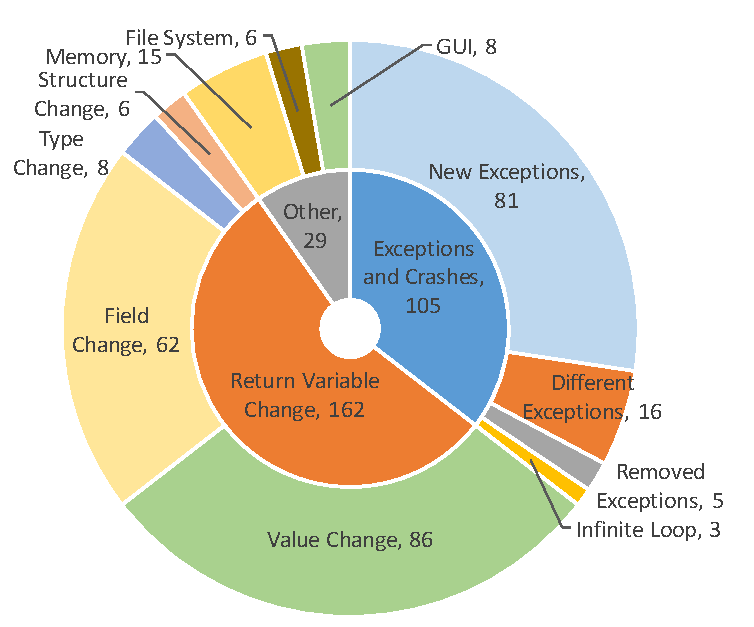
\includegraphics[width=0.4\textwidth]{backward/figs/Behavior.pdf}
	\caption{BBI Distribution on Incompatible Behaviors}
	\label{figure:behavior}
	\vspace{0.3cm}
\end{figure}

\subsubsection{Invocation Constraints}

We further investigated the conditions under which BBIs can be invoked, and identified the following five major types of such conditions. 

\textbf{Always} indicates that the BBI always happens as long as the corresponding API method is invoked.

%However, it should be noted that such incompatibilities may not be easily detected in the client software, because the relevant API method may not easily invoked, and the incompatible behavior (e.g., changed return value) may be overwritten by other code and thus cannot be observed under certain conditions. %Such incompatibilities can be easily detected by regression unit testing, so they are more likely to be intended behavioral changes.

\textbf{Error} indicates that the BBI happens only when an error happens. An example is the change of error message when a network error is invoked. 

\textbf{Environment} indicates that the BBI happens only under certain environments of the application (e.g., operating systems, language settings). 

\textbf{Multiple APIs} indicates that a number of other API methods must be invoked before the backward incompatible API method to invoke the BBI. Example~\ref{example:Method} belongs to this category. 

\textbf{Input} indicates that the BBI happens when a certain input value is fed into the corresponding API method. Specifically, we divide this category into five sub-categories. \textit{Trivial Value} indicates a null pointer or an empty string / list as the input. \textit{String Format} indicates that strings with specific structure as the input. \textit{Special Field} indicates that objects with specific values at a certain field as the input. \textit{Special Value} indicates that certain primitive values (not including strings) as the input. \textbf{Special Type} indicates the argument of the API method must be of a specific subtype of its parameter type.

The distribution of 296 backward incompatibilities in the above categories is presented in Figure~\ref{figure:condition}. We can observe that, the top 3 categories of invocation conditions are \textit{Always}, \textit{Specific Value}, and \textit{String Format}. The commonality among the 3 categories of BBIs is that they can be invoked with one API method invocation. By contrast, the BBIs requiring multiple API methods to invoke are not common in those detected by regression testing. 


%253 of 296 (85.5\%) detected BBIs alway happen whenever the API method is invoked, or happen under certain inputs. In the \textit{input} category, 129 BBIs are invoked by simple input values, while the rest 32 are fields of complicated inputs. 



%The dominance of category \textit{Always (\textbf{AL})} may be because they are easier to detect.

%Also, we observed that the distribution of categories in some projects are uneven. For example, JSoup, as the most popular HTML parser with 36 incompatibilities in total, contributes 30 of the 43 incompatibilities in the category of  \textit{String Format (\textbf{SF})}. Actually, while incompatibilities are distributed evenly in general libraries like JDK and Android. For library of narrower usage such as JSoup, Elastic Search and SnakeYaml (a data presentation library), more than 70\% of incompatibilities concentrate in \CodeIn{Jsoup.parse()}, \CodeIn{Client.prepareSearch()} and \CodeIn{Yaml.dump()}, the most widely used APIs in the libraries. 

%\begin{table}
	\center 
	\caption{\label{table:Cond} Invocation Conditions of Incompatibilities}
	\begin{tabular}{|l|r|r|r|r|r|r|r|r|r|}
		\hline
		&        &                &             &            &              & \multicolumn{4}{c|}{Input}\\
		\cline{7-10}
Subject & AL & ER & EV & ST & MA & TR & SF & FI & SV\\
\hline
JDK & 2 & 2 & 2 & 0 & 6 & 2 & 2 & 6 & 13\\
and & 18 & 4 & 2 & 1 & 4 & 11 & 3 & 4 & 9\\
log & 2 & 0 & 0 & 1 & 0 & 0 & 0 & 0 & 1\\
mav & 13 & 0 & 0 & 0 & 0 & 0 & 6 & 0 & 0\\
buk & 5 & 0 & 0 & 0 & 0 & 1 & 0 & 0 & 1\\
bea & 0 & 0 & 0 & 0 & 0 & 0 & 0 & 0 & 0\\
cod & 2 & 0 & 0 & 0 & 0 & 0 & 0 & 0 & 4\\
fil & 2 & 0 & 0 & 0 & 0 & 0 & 0 & 0 & 0\\
cio & 1 & 2 & 0 & 0 & 0 & 0 & 0 & 0 & 0\\
ela & 6 & 2 & 0 & 2 & 4 & 2 & 1 & 7 & 0\\
htt & 8 & 4 & 0 & 0 & 3 & 3 & 0 & 7 & 7\\
jod & 5 & 1 & 0 & 0 & 0 & 8 & 0 & 0 & 3\\
jso & 0 & 1 & 0 & 0 & 2 & 1 & 30 & 0 & 2\\
neo & 3 & 0 & 0 & 0 & 0 & 1 & 0 & 2 & 0\\
sna & 25 & 2 & 0 & 6 & 2 & 2 & 1 & 6 & 5\\
\hline
\textbf{Total} & \textbf{92} & \textbf{18} & \textbf{4} & \textbf{10} & \textbf{21} & \textbf{31} & \textbf{43} & \textbf{32} & \textbf{45}\\
\hline
	\end{tabular}
		\vspace{1cm}
\end{table}
\begin{figure}
	\centering
	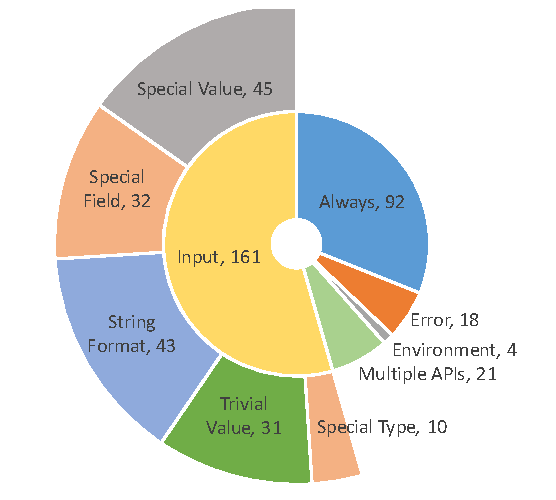
\includegraphics[width=0.4\textwidth]{backward/figs/Condition.pdf}
	
	\caption{BBI Distribution on Invoking Conditions}
	
	\label{figure:condition}
	\vspace{0.3cm}
\end{figure}


\subsubsection{Reasons for Bringing in BBIs}

Since the library developers revised the test cases to accommodate the changes, we can find out the reasons and the purposes of the behavior change from the revised test code. We identified the following 3 major categories of reasons, which contains 13 sub-categories. 

\textbf{Usage Change} indicates that the library developers expect to keep the normal behavior of the library, but also expect client developers to change their usage pattern. This category has 4 sub-categories, which are \textit{API Pattern Change} indicating changes on expected API sequences, \textit{Enforce Rules} indicating rejecting of some poor input, \textit{Enable Poor Inputs} indicating the support to some poor input, and \textit{Input Format} indicating the change on the format of string type inputs. 

\textbf{Better Output} indicates that the library developers expect to change the normal behavior of the API, while not expecting client developers to change their input. This category also has 5 sub-categories, which are \textit{More Reasonable Output/Effect} indicating behavior change of an API method under a normal input to make it more reasonable\footnote{For example, in log4j 2.0.2, the time stamp on the log is changed from when the log is initialized to when the time stamp line is printed. }, \textit{Change Default Setting} indicating changing of the default setting (often a constant such as the default screen size), \textit{Error Message} indicating change of reported errors, \textit{Explicit Report} indicating explicitly throwing exceptions for errors, and \textit{Output Format} indicating format change of string output. 

\textbf{Other} indicates reasons not in the above 2 categories, including \textit{Exposure of Internal Structure Change}, \textit{Signature Change exposed with Reflection}, and \textit{Upgrade Library}, in which the first two categories are regression faults.  

The distribution of 296 backward incompatibilities in the above categories is presented in Figure~\ref{figure:reason}. From the table, we can see the top 3 reasons for bringing incompatible behaviors are \textit{More Reasonable Output/Effect}, \textit{Output Format}, and \textit{Enforce Rules}. We also find that, \textit{Enable Poor Inputs}, the opposite of \textit{Enforce Rules}, is the 4th popular reasons. Such contradiction reflects hesitation of library developers on whether responsibilities (e.g., input validation checking) should be at the library side or client side. Also, we did observe library developers moving back-and-forth on some incompatibilities. For example, in SnakeYaml, whether the dump output should include class name of the data value is changed 3 times through versions 1.3 to 1.6. Furthermore, although \textit{More Reasonable Output/Effect} is the largest sub-category in \textit{Better Output}, 93 of 165 BBIs in the category are not semantic changes, but presentation changes (e.g., error message, explicit exceptions, output formats). The 17 BBIs on change of default setting also related to client developers' preference. To sum up, we have the following observation. 

\medskip\vspace{+0.05cm}
\noindent\begin{tabular}{|p{16cm}|}
	\hline
	\textbf{Observation 4:} Developers bring in a large portion of BBIs because they want to allow more or less inputs, or change the output presentation or option. This implies that the root cause of most BBIs is the different requirement of client developers, so the BBIs can be avoided if library developers understand requirement better (e.g., through surveys or code statistics on client projects), or have design for dual support.
	\\
	\hline
\end{tabular}
\medskip

%\begin{table}
\centering
	\caption{\label{table:reason} Reasons for Bringing in Incompatibilities}
	\begin{tabular}{|p{0.5cm}|R{0.5cm}|R{0.5cm}|R{0.5cm}|R{0.5cm}|R{0.5cm}|R{0.5cm}|R{0.5cm}|R{0.5cm}|R{0.5cm}|R{0.5cm}|R{0.5cm}|R{0.5cm}|R{0.5cm}|}
		\hline
		&  \multicolumn{5}{c|}{Usage Change}      &   \multicolumn{5}{c|}{Behavior Change}  & \multicolumn{3}{c|}{Other}\\
		\cline{2-14}
Sbj & AP & ER & EL & RE & IF & RB & CD & EM & DE & OF & IS & SR & UL\\
\hline
jdk & 6 & 13 & 3 & 1 & 0 & 7 & 2 & 0 & 1 & 1 & 1 & 0 & 0\\
and & 4 & 6 & 8 & 1 & 0 & 14 & 8 & 0 & 3 & 7 & 2 & 3 & 0\\
log & 2 & 1 & 0 & 0 & 0 & 1 & 0 & 0 & 0 & 0 & 0 & 0 & 0\\
mav & 0 & 0 & 1 & 1 & 0 & 2 & 0 & 1 & 0 & 0 & 1 & 1 & 12\\
buk & 0 & 1 & 0 & 0 & 0 & 0 & 0 & 0 & 0 & 2 & 0 & 4 & 0\\
bea & 0 & 0 & 0 & 0 & 0 & 0 & 0 & 0 & 0 & 0 & 0 & 0 & 0\\
cod & 0 & 4 & 0 & 0 & 0 & 2 & 0 & 0 & 0 & 0 & 0 & 0 & 0\\
fil & 0 & 0 & 0 & 0 & 1 & 0 & 0 & 0 & 0 & 0 & 0 & 0 & 1\\
cio & 0 & 0 & 0 & 0 & 0 & 1 & 0 & 0 & 2 & 0 & 0 & 0 & 0\\
ela & 1 & 2 & 3 & 5 & 0 & 3 & 1 & 4 & 0 & 2 & 1 & 2 & 0\\
htt & 2 & 4 & 5 & 3 & 1 & 10 & 2 & 0 & 1 & 4 & 0 & 0 & 0\\
jod & 0 & 3 & 1 & 6 & 1 & 0 & 1 & 0 & 1 & 3 & 1 & 0 & 0\\
jso & 0 & 2 & 8 & 0 & 3 & 13 & 0 & 0 & 0 & 10 & 0 & 0 & 0\\
neo & 0 & 3 & 1 & 0 & 0 & 1 & 1 & 0 & 0 & 0 & 0 & 0 & 0\\
sna & 2 & 2 & 3 & 2 & 0 & 1 & 2 & 16 & 1 & 15 & 3 & 2 & 0\\
\hline
\textbf{Tot.} & \textbf{17} & \textbf{41} & \textbf{33} & \textbf{19} & \textbf{6} & \textbf{55} & \textbf{17} & \textbf{21} & \textbf{9} & \textbf{44} & \textbf{9} & \textbf{12} & \textbf{13}\\
\hline
	\end{tabular}	
	\vspace{1cm}
\end{table}

\begin{figure}
	\centering
	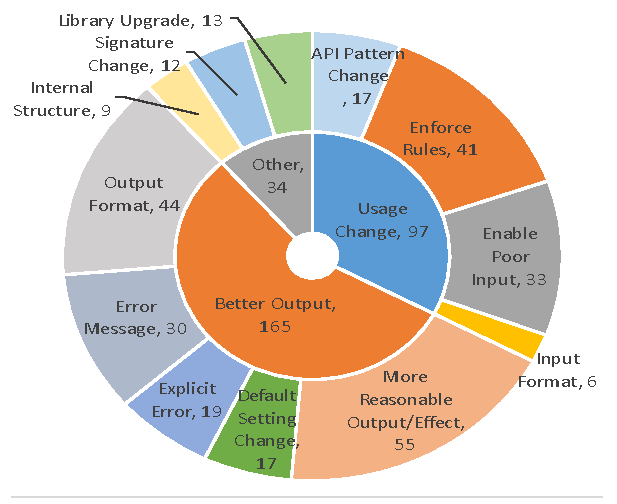
\includegraphics[width=0.4\textwidth]{backward/figs/Reason.pdf}
	
	\caption{BBI Distribution on Reasons}
	
	\label{figure:reason}
	\vspace{0.3cm}
\end{figure}


\section{Real-world Bug Study}
\label{sec:studybug}
In this section, to answer the \textbf{RQ4} and \textbf{RQ5}, we present the study result on real world bug reports related to BBIs, and explore how BBIs are affecting the client software developers. The basic information of the collected bug reports are presented in Table~\ref{table:basicbug}. 

%In the following subsections, we first identify bug reports that are related to signature incompatibilities, and cross-software duplicate bug reports. Then, we categorize bug-inducing behavior incompatibilities and map them back to categories in our library study, and study their documentation status. Finally, we study how these bug are fixed or resolved by library developers and client developers. 

\subsection{Collection of Bug Reports}
To collect bug reports caused by BBIs. We searched two large on-line open bug repositories: JIRA and GitHub, on their project-specific bug report search engine. Specifically, we used as keywords the combination of terms related to software upgrading (e.g., ``upgrade'', ``update'', ``version''), and the names of the software libraries listed in Table~\ref{table:basicInfo}. From the collected bug reports, we \textit{randomly} selected 500 bug reports, and carefully inspected these bug reports. During the inspection, we read the developers' comments and other references from the bug report to check whether they are confirmed by the developers to be caused by BBIs, and retain all the bug reports that are caused by BBIs. 

We collected only bugs that are closed before Jan. 1st 2015 and never re-opened after that. We believe that these bugs are not likely to be re-opened so their status should be confirmed. We collect both bugs that are closed and fixed and bugs that are closed but not fixed due to developers' decision. 

The reason is that, BBIs bugs are related to both software libraries and client software, so they can be fixed either at the library side or at the client side. Also, there are cases that a BBI bug is never fixed because the software library developers refuse to revert their changes, and the client developers did not find a way to work around it. In such cases, the developers may choose to not to support the new version of software library (not likely for runtime libraries such as OpenJDK and Android because not supporting the updated platform will cause dysfunction in client software), or have the users to tolerate the bug if the bug is relatively minor. 

With the process above, we collected 126 bugs, and divided these bugs into two groups: \textit{library bugs} that are submitted to software library projects that have BBIs, and \textit{client bugs} that are submitted to software client projects because they triggers BBIs of their software libraries. The breakdown of collected bugs is shown in Table~\ref{table:basicbug}.

\begin{table}
	\center
	\caption{\label{table:basicbug} Basic Information of Bugs}
				
	\begin{tabular}{|l|r|r|r|}
		\hline
		Subject & Library Bugs& Client Bugs & Total\\ 
		\hline
		Java SDK &        8      &     10   & 18   \\
		Android &         13     &     64   & 77  \\
		Other   &         29     &    2    & 31  \\
		\hline
			Total   & 50             &  76     & 126     \\
		\hline
	\end{tabular}
	\vspace{+0.3cm}			
\end{table}

From the table, we can observe that, as we used a random selection of bugs, the majority of selected bug reports are from Android and Java SE. The reasons are two fold. First, Java SE and Android are much popular than other software libraries studied. Second, Java SE and Android are both runtime platforms, so that client software developers do not have control on which version of JVM and Android system their software will be executed on. Therefore, BBIs may be revealed after a Java or Android update at the users' side, and get reported to the client software developers. This also explains another observation that, the majority of bugs of Android and Java SE are client bugs, while the majority of bugs of other libraries are library bugs, because Android and Java BBIs are more likely to be reported by end users, while BBIs in other libraries are more likely to be reported by client software developers to library software as library bugs. Sampling from unbalanced bug sets is difficult. Random sampling will be ruled by dominating classes (e.g., JVM and Android). Giving quota to classes, samples will not reflect the actual data distribution, and proper quota size needs to be determined. We chose random sampling in our study to see the actual impact of BBIs in the field. 

%Obviously, Java SE is used in all Java projects. Furthermore, in our previous study on API popularity among 10,000 random Github projects~\cite{QSICStudy}, Android libraries are used in 34\% of the 10,000 projects , while Apache Http, which ranks the 3rd after Java SE and Android, is used in only 10\% of the projects. By contrast, most of the other libraries in our study are packaged with the client software. Thus, client software developers are able to test the backward compatibility of a new software-library version, and work around the backward incompatibilities before the software is released to the users. 

%\subsubsection{Selecting Test Errors / Failures for Manual Inspection}

%When selecting test errors and failures for manual inspection, we expect our subset to be selected random, as well as representative enough to cover all the studied subject libraries. Therefore, we use the strategy of senate-house election. Specifically, we first randomly selected 1 test error / failure from each subject library, and then we randomly select 100 test errors / failures from all the rest test errors and failures. So, finally we form a selected subset with 127 test failure and errors, from which we identified 1xx behavioral incompatibilities with manual inspection. 

\subsection{Study on Bug-Inducing BBIs}

In this subsection, we categorize the bug-inducing BBIs and compare them to the BBI distribution in our library study. Specifically, among the 126 bugs, we find 13 bugs (12 client bugs from Android and 1 library bug from http-core) that can be directly mapped to the BBIs found in our library study. This shows that the test cases in regression testing are far from sufficient for identifying all bug-inducing BBIs, but it also implies that, if the regression testing results can be well documented or conveyed to client developers in better ways, some bugs can be avoided. 


%\subsubsection{Signature Incompatibilities}

%Since the bug reports are randomly collected, some of the bug reports are related to signature-level incompatibilities. As we mentioned in Section~\ref{sec:intro}, since signature-level incompatibilities fail compilation, they are not likely to result in real world bugs. 

%Among the 144 bug reports, we do find 18 of then related to signature-level incompatibilities. Specifically, 6 of the 18 bugs are library bugs, which are reported by client developers to request of the recovery of a removed API method. Other 6 of the 18 bugs are runtime errors from client software running on Android, Java, and Bukkit. Because these libraries serve as runtime environments, when automatic updates happen, the software running on them will throw exceptions such as ``NoSuchFieldException'' or ``UnSupportedOperationException''. 

%The rest 6 of the 18 bug reports are more interesting. As for these bugs, the developers of relevant client software use reflections to invoke the API methods with signature changes, or use ``instanceof'' operations, or downcasts on the classes whose inheritance hierarchy has changed. Thus the signature incompatibilities become latent, and cannot be detected by compilers. It should be noted that, 4 of the 6 bug reports are related to Android. Reflection is encouraged in Android to address backward incompatibilities (i.e., call different API methods for different Android versions), so it seems that reflection serves as a double-edge sword here. 

%\framebox{\parbox{\dimexpr\linewidth-2\fboxsep-2\fboxrule}{\textbf{Finding 1}: An important group of runtime bugs related to signature incompatibilities are due to invoking library methods with reflection or checking class hierarchy of the library.}}Besides the 18 bug reports discussed above, the rest 126 bug reports are all related to behavioral incompatibilities. 


%\subsubsection{Behavioral Incompatibilities}

Before we perform more in-depth investigation, we first manually scanned the bug reports to detect \textit{cross-software duplicate bug reports}. Duplicate bug reports inside a project are typically labeled and we did not select them when collecting our bug report set. However, different client software may fail due to a same BBI of a same library, so these client bug reports are ``duplicate'' with each other. After the duplicate-bug-report detection, we identified 112 BBIs as presented in Table~\ref{table:basicIncomp}. 

\begin{table}
	\center 
	\caption{\label{table:basicIncomp} Bug-Causing BBIs}
	
	\begin{tabular}{|l|r|r|r|}
		\hline
		Subject & Cause Library Bugs& Cause Client Bugs & Total\\ 
		\hline
		JDK &        8      &     10   & 18   \\
		Android &         13     &     51   & 64  \\
		Other   &         29     &    1    & 30  \\
		\hline
		Total   & 50             &  62      & 112     \\
		\hline
	\end{tabular}
	\vspace{+0.3cm}		
\end{table}

\subsubsection{Incompatible Behaviors}

\begin{example}
	\begin{verbatim}
In Android 4.4, SMS apps are no longer able 
to send SMS to the SMS provider (rejected 
silently) in the Android system, unless they 
are reset to receive a broadcast 
SMS_DELIVER_ACTION. 	
 \end{verbatim}
	\caption{Bug-408: Be able to configure as a default 
		SMS app in KitKat (\small{from WhisperSystems/TextSecure})} 
	\label{example:sys}
\end{example}

The breakdown of bug-inducing BBIs per incompatible behaviors is presented in Table~\ref{table:behavior}. Note that, in our bug study, we use the same categories as defined in Section~\ref{subsec:cats}. For incompatible behaviors, we found 2 BBIs that cannot be put into any defined categories, so we add a new category \textit{Sys. Event}, which indicates changes in system events (Example~\ref{example:sys}).

\begin{table}
	\center
	\caption{\label{table:behavior} Categorization of Incompatible Behaviors}
			
	\begin{tabular}{|l|l|r|r|r|r|r|r|r|}
		\hline
		\multicolumn{2}{|l|}{Behavior} & \multicolumn{2}{|c|}{Android} & \multicolumn{2}{|c|}{JDK} & \multicolumn{2}{|c|}{Other} & All\\
		\cline{3-8}
		\multicolumn{2}{|l|}{}      & L & C & L & C & L & C& \\
		\hline
\NameEntry{2}{Exception and Crash}&New Exception &2 &  21&5&5&13&1 & 47\\ 
		&Infinite Loop &0 & 0  & 1&0& 0&  0& 1 \\ 
		\hline
		\NameEntry{4}{Ret. Var. Change}& Value Change &1 & 0& 0&1&2&0&4 \\
		& Field Change & 1 & 2 & 1 & 2 & 7 & 0 & 13\\
		& Type Change&1     & 2 &0 & 0 & 1 & 0 & 4  \\
		& Structure Change&0    & 0 & 0&1&3   & 0 & 4 \\
		\hline
		\NameEntry{4}{Other Effects}& Memory&3 & 4  &0&0&1 & 0& 8 \\         
		&  GUI     &5     &19 & 0&1 &1  &  0 & 26 \\
		& File Sys.   &0     &  2 & 0 &0 & 1&  0 &3  \\
		& Sys. Event    & 0    &  1 & 1 & 0& 0&  0 &2  \\		
		\hline 
	\end{tabular}	
\end{table}

In the table, Columns 2-3 present the number of library bugs (denoted as L) and client bugs (denoted as C) from Android. Columns 4-7 present similar data for Java and Other subjects. Column 8 presents the total of each line. Since Android and JDK dominates our bug report study set, in the rest of the paper, when comparing bug study results and library study results, we provide both overall library study results, and library study results for JDK and Android combined. From Table~\ref{table:behavior}, we have the following observations. 

First, \textit{New Exception} and \textit{Infinite Loop} account for 48 of the 112 (43\%) BBIs, which is higher than their proportion in the library study (28\% overall, 30\% for JDK+Android). These behaviors may be more likely to be reported as bugs due to their severity.

Second, \textit{Value Change} accounts for 4 BBIs (3\%), which is much smaller than its share in library study (29\% overall, 18\% for JDK+ Android). But \textit{Field Change} accounts for 13 BBIs, which is much more than \textit{Value Change} despite its lower share in library study. 

Third, categories \textit{Different Exception} and \textit{No Exception} do not cause any bugs in our data set. This may be because client developers tend to avoid exceptions in their code so they are not affected. This also indicates that such changes are safer at the library side. 

\begin{example}

		\begin{verbatim}
	In Android 4.4, a method that update the 
	padding setting must be invoked before 
	showing the date information, otherwise, 
	part of the date information can not be seen.
		\end{verbatim}
	\caption{Bug-46:Bold ZeroTopPaddingTextView displays cut off on 4.4 (\small{from derekbrameyer/android-betterpickers})} 
	\label{example:ui} 
	
\end{example}
	
Fourth, GUI changes accounts for 26 BBIs (22.3\%), which is the second largest category in bug study, but its share in library study is only 3\% overall. The large number of GUI-change BBIs may be related to the large proportion of Android-related bugs in our bug set. Although these BBIs may be specific to Android framework, they are still important and representative because of the popularity of Android apps, and the existence of similar frameworks. We discovered that, most bug-inducing GUI BBIs are changing settings of UI controls and thus affecting presentation. Examples of the settings include the position to put notification bars (top or bottom), box widths, etc. Example~\ref{example:ui} presents a GUI-related bug. The bug report is caused by a BBI between Android 4.3 and Android 4.4 about the changed value of padding settings. It should be noted that, user interface bugs are not just decoration problems, and they may largely affect software usages (i.e., information cannot be seen, or buttons go outside the screen and cannot be clicked). In general, we have the observation as follows.\\



\medskip
\noindent\begin{tabular}{|p{16cm}|}
	\hline
	\textbf{Observation 5:} Distribution of BBIs in library study and field bug study is mismatched on the incompatibility behavior categories. New Exception, GUI Changes, and other side-effects account for a higher proportion in field bug study, while other categories of BBIs account for a lower proportion.\\
	\hline
\end{tabular}
\medskip
\vspace{+0.2cm}




%Since Android and JDK dominates our bug report study set, in the rest of the paper, when comparing bug study results and library study results, we provide both overall library study results, and library study results for JDK and Android combined. 



%this proportion of 45\% is much more than their proportion (28\% overall, 30\% JDK+Android) in the library study at Figure~\ref{figure:behavior}). This implies that, library developers should be very careful when bringing in incompatibilities in this category. Also, simpler and more scalable techniques that target at unhandled-exception-related changes in the software library may be quite effective in detecting these bug-inducing backward incompatibilities. 


%(50\% overall, 33\% JDK+Android). It is possible that such incompatibilities are relatively simple and are thus easier for client developers to handle or they are not breaking client code bad enough to result in bug reports. This also shows that unit testing, which does well in checking return values under simple inputs and context, is not sufficient for identifying bug-inducing incompatibilities. 





%Such settings are often changed to achieve better presentation of the Android System GUI, but they may also affect the GUI of Android apps. By contrast, the GUI BBIs discovered in our library study are mostly about UI control actions such as dialog not showing or cursor not moving. 

	



\subsubsection{Invocation Constraints}

\begin{table}
	\center
	\caption{\label{table:condition} Categorization of Invocation Conditions}
		
	\begin{tabular}{|l|l|r|r|r|r|r|r|r|}
		\hline
		\multicolumn{2}{|l|}{Conditions} & \multicolumn{2}{|c|}{Android} & \multicolumn{2}{|c|}{Java} & \multicolumn{2}{|c|}{Other} & All\\
		\cline{3-8}
		 \multicolumn{2}{|l|}{}      & L & C & L & C & L & C& \\
		\hline
		\multicolumn{2}{|l|}{Always} &5 &  14  &2  & 1   & 2 &0& 24 \\ 
		\hline
		\multicolumn{2}{|l|}{Environment}  &0 & 1   & 0 & 0   & 1 &0& 2 \\ 
		\hline
		\multicolumn{2}{|l|}{Special Type} &0 &  2  & 0 &  0  & 2 &0& 4 \\ 	
		\hline		
		\multicolumn{2}{|l|}{Multiple APIs} &4& 21 & 1 & 5& 7 &1& 39 \\ 	
		\hline		
		
		\NameEntry{4}{Input}& Trivial Value &0 &  0  & 1 &  0  & 2 &0& 3 \\ 
		& String Format &2 &   2 & 3 &   3 & 6 &0& 16 \\ 
	    & Specific Field &0 & 4   & 0 &  0  & 0 &0& 4 \\ 
		& Specific Value &2 &  7  & 1 &  1  & 9 &0& 20 \\ 
		\hline
	\end{tabular}
	\vspace{+0.3cm}			
\end{table}


The breakdown of bug reports according to BBI-invoking conditions is presented in Table~\ref{table:condition}. From the table, we have the following observations. 

First of all, 24 of 112 (21\%) BBIs always happen (compared to 31\% overall and 22\% in JDK+Android in the library study), causing at least 15 client-side bugs. Second, only 2 of the BBIs are related to the environment. This may be largely due to the platform independence of Java, so we doubt whether this conclusion can be generalized to other programming languages. 
Third, 39 BBIs (35\%) occur only after certain other API methods are invoked and thus belong to the category of \textit{Multiple API}, compared to 7\% overall and 11\% JDK+Android in the library study. This actually implies that a lot of BBIs happen under special usage scenarios which are not covered by the library-side test code. In such cases, client code may be a good source to extract suitable test cases for detecting BBIs in a software library. 
Fourth, no BBIs fall into the \textit{Error} category of invocation-condition, which shows that BBIs in this category are less likely to cause client bugs or the client bugs they cause are difficult to detect. In general, we have the observation as follows.\\

\noindent
\begin{tabular}{|p{16cm}|}
	\hline
	\textbf{Observation 6:} Distribution of BBIs in library study and field bug study is mismatched on invocation constraints. Multiple APIs account for a much higher proportion in field bug study, compared to its share in library study. This implies that regression testing may need to be strengthened for usage patterns involving multiple API methods. 	
%	these categories (e.g., automatic GUI oracle checking, including multiple API usage patterns from client code into regression test suite)
	\\
	\hline
\end{tabular}
\medskip
\vspace{+0.05cm}
%\subsubsection{Call Backs}
%One interesting finding in the 112 studied incompatibilities is that, 6 of them are related to call backs. All 6 incompatibilities are from Android bugs (4 client bugs and 2 library bugs). 

%One example of call-back-related incompatibilities is \textit{Bug-62100: ``WebViewClient.onPageFinished() called multiple times''} of Android system. The bug is a library bug about a backward incompatibility between Android 4.3 and Android 4.4. Specifically, in Android 4.3, this call back method is called only once when a web view with multiple frames is closed. However, in Android 4.4, the developers added a new method \CodeIn{didFinishLoad(...)}, and invoke it when closing each frame (the added method is shown in the code sample below). Note that this method invokes the call back method \CodeIn{onPageFinished(...)}, so in Android 4.4, the call back method is called multiple times when closing a web view with multiple frames. Such a  change may cause severe problem, if the client developers close some resources (closing a closed resource may cause exceptions) or change some global objects such as counters, in the call back. This bug has been reported to and fixed by Android developers. In the fix, the developer added line 4 to check whether the frame to be closed is the main frame, and invoke the call back method only if the frame is a main frame.
	%\vspace{-0.2cm}

%\begin{CodeOut}
%\begin{alltt}
%1 @Override
%2 public void didFinishLoad(long frameId, String validatedUrl, 
%3   boolean isMainFrame) \{
%4+    if (isMainFrame)
%5       AwContentsClient.this.onPageFinished(validatedUrl);
% 	 ...
% \} 
%\end{alltt}	
%\end{CodeOut} %
%	\vspace{-0.2cm}
%Call-back backward incompatibilities can easily happen, because library developers may simply change the way they are calling a certain method inside their code, without noticing that this method is being overridden by client developers. Also, call-back backward incompatibilities are difficult to avoid, because library developers often cannot make any assumptions on the content of the call back. 
		
\subsection{Documentation Study}
\label{subsubsec:docIncomp}
To answer the third research question, we further studied the documentation status of the bug-inducing BBIs. Since these BBIs are bug inducing, we predict that they may be more poorly documented then the BBIs detected from cross-version testing (34\% documented), and the results shown in Table~\ref{table:documentation} confirm our guess. In Table~\ref{table:documentation}, the first column presents the documentation status (and the place if documented). The rest columns are organized similar to Table~\ref{table:behavior}. 

\begin{table}
	\center
	\caption{\label{table:documentation} Documentation Status of BBIs}
	\begin{tabular}{|l|l|r|r|r|r|r|r|r|}
		\hline
		\multicolumn{2}{|l|}{Behavior} & \multicolumn{2}{|c|}{Android} & \multicolumn{2}{|c|}{Java} & \multicolumn{2}{|c|}{Other} & All\\
		\cline{3-8}
		\multicolumn{2}{|l|}{}      & L & C & L & C & L & C& \\
		\hline
		\multicolumn{2}{|l|}{No Doc.} &12&43&7&6&  29&  1  & 98  \\
		\hline
		\multirow{3}{*}{Doc.}&Release Notes &1   & 1&1&3& 0 &  0 & 6  \\
		&JavaDoc       & 0  &  3 &0&1& 0 &   0  & 4  \\
		&Migration Guide &  0  & 4   &0&0& 0& 0  &  4  \\
		\hline 
	\end{tabular}
	\vspace{+0.3cm}	
\end{table}

From Table~\ref{table:documentation}, we can see that bug-inducing behavioral BBIs are very poorly documented. Only 14 (13\%) BBIs are documented.  Also, the documented changes are relatively scattered, especially for Android (in release notes, JavaDocs, and Migration guides). Also, 8 client bugs of Android and 4 client bugs of Java are related to documented behavioral changes. This implies that we may need a better way than documentation to convey the information of behavioral change and remind client software developers about such changes. 
		
\subsection{Bug Resolution Study}
		

To answer \textbf{RQ5}, we further studied how the real world bugs related to BBIs are resolved (note that they may be not fixed). Cross-software duplicate bugs may be fixed differently in different client software, so we view them as separate bugs in this subsection. 

\subsubsection{Resolution of Library Bugs}

The breakdown of bugs according to how they are resolved is shown in Table~\ref{table:libfix}. The first two columns present the types of resolution. If a library bug is fixed, we check whether it is fixed by a simple revert of the previous change, a patch of the previous change, or library developers decided to support both the previous behavior and the new behavior (typically by adding a parameter, and set either the previous behavior or the new behavior as default). If a library bug is not fixed, we study how library developers response to the bug report, and check whether it is intended behavior, or the developer is reporting a behavioral change on internal APIs which should not be used by client developers. 

\begin{table}
	\center
	\caption{\label{table:libfix} Resolution of Library Bugs}
			
	\begin{tabular}{|l|l|r|r|r|r|}
		\hline
		\multicolumn{2}{|l|}{Resolution} & Android & Java & Other & All\\
		\hline
		\NameEntry{3}{Fixed}& Reverted & 1   & 0 & 2    &   3\\
		& Patched&  6 &  4  &  16  &   26 \\
		& Double Support& 0  &  0  & 1   & 1   \\
		\hline
		\NameEntry{3}{Not Fixed}& Intended& 5  & 2 & 10  &  17 \\         
		& Discouraged     & 1  &2  &  0  & 3  \\		\hline 				
	\end{tabular}	
	\vspace{+0.3cm}	
\end{table}

From Table~\ref{table:libfix}, we have the following observations. 
First, 20 of 50 library bugs are not fixed. The major reason is that the behavior change described in the bug report is intentional. It should be noted that, since these behaviors are reported as library bugs, they may already cause some bugs or at least test failures at the client side, although the client bug may not be reported. Second, among the 30 bugs that are fixed, most of them are patched, which shows that the many bug-inducing BBIs are caused by side effect of other productive changes. 

\subsubsection{Resolution of Client Bugs}
The breakdown of client bugs according to how they are resolved is shown in Table~\ref{table:clifix}. The first two columns present the types of resolution. If a client bug is fixed, we check whether it is fixed by (1) changing the incompatible API method to another one; (2) changing the arguments of the incompatible API method to other constants, variable, or expressions; (3) adding an API invocation to set a certain internal-state field before or after the invocation of the incompatible API method; (4) converting the return value of the incompatible API invocation to the original value; (5) a global structural code change; (6) updating libraries; (7) changing configuration of software; or (8) bypassing the incompatibility behavior by skipping software features (see Example~\ref{example:libfix}).

\medskip
\begin{example}	
\begin{verbatim}
The cause of the bug is that, "ResourceNotFound 
Exception" is thrown in Android 5.0 when an 
"overall scroll glow drawer" is requested. 
In the fix, the client developers simply catch 
the exception without doing anything with it. 
Therefore, the request of "overall scroll glow 
drawer" is actually bypassed. 
\end{verbatim}
\caption{Bug-969: Android 5.0 crash when trying to open the app (\small{from open-keychain/open-keychain})} 
	\label{example:libfix}
\end{example}


%An example of bypassing is the resolution of \textit{}. 

For the client bugs that are not fixed, we discovered two resolutions. The first resolution is that the client developer simply decided to wait until a new version library is released. One reason of such resolution is that, the BBI is caused by a regression bug, so the client developer waits for the library developers to release a bug-free version. Another reason (and the major reason in our study) is that, the BBI affects a third-party library that the client developers are relying on. Since the client developers cannot change the code of the third-party library (sometime they even do not have access to the source code), they are not able to resolve the BBI, and have to wait for the new version of the third party library. The second solution is that, the client developer simply tolerate the behavior change (if the BBI does not cause crashes). They may simply ask their users to get used to the new behavior such as a UI change, or transfer the BBI to downstream developers. 

\begin{table}
	\center
	\caption{\label{table:clifix} Resolution of Client Bugs}
	\begin{tabular}{|l|l|r|r|r|r|}
		\hline
		\multicolumn{2}{|l|}{Resolution} & Android & Java & Other & All\\
		\hline
		\NameEntry{8}{Fixed}& Change API & 1   &  2 &   0  &  3  \\
		& Change Input& 13  & 0   &  1  & 14 \\
		& Add Set Field& 17   & 1   &   0  &  18  \\
		& Return Convert& 6  & 0   &  0  &  6  \\
		& Structural&  8 &   5 &   0  &  13  \\
		& Config&    2 &   0 &  0  & 2   \\
		& Lib. Update&  2   &  0  &  0     &  2  \\ 
		& Bypass&   4  &  0  & 0  &  4  \\ 
		
		\hline
		\NameEntry{2}{Not Fixed}& Wait Lib. Fix& 4  & 2 &  0  & 6  \\         
		& Tolerate  & 7  & 0 &  1  &  8 \\		
		\hline 
	\end{tabular}	
	\vspace{+0.3cm}		
\end{table}

Table~\ref{table:libfix} shows that 14 client bugs are not fixed. Note that, we find that most developers are willing to and have tried to fix the bugs, but BBI-related bugs are more difficult to fix, because they typically involve code written by other people. Regarding the fixed client bugs, we have the observation as follows. \\


\noindent\begin{tabular}{|p{16cm}|}
	\hline
	\textbf{Observation 7:} 41 of the 62 fixed client bugs are fixed through small changes including changing API, changing input value, add an API to set field, or convert the return value to the original value. \\
	\hline
\end{tabular}
\\

We present an example of client bug fixing with ``Add an API to set field'' in Example~\ref{example:fix}. The corresponding BBI is that, for Android 5.0, if the developer wants to start a service with an intent, the type of the intent must be explicitly set with the method \CodeIn{setClass(...)}, and the method \CodeIn{startService(...)} will check the \CodeIn{class} field of the intent and throw exceptions if the value is null. %For this example, if we can summarize the addition of field checking in the library code, it will be not difficult to generate the patch code based on the summary. 

\begin{example}
	\begin{verbatim}
 Intent intent = new Intent(
 Actions.NOTIFICATION_SET_FOR_DEVICE); 
+intent.setClass(context, 
     NotificationIntentService.class);
 intent.putExtra(BundleExtraKeys.DEVICE_NAME
     , deviceName);          
 ...
 context.startService(intent); 
	\end{verbatim}
	\caption{Fix: Bug-812: Lollipop notification settings won't work \small{(from klassm/andFHEM)}} 
	\label{example:fix}
\end{example}

		

\subsubsection{Reporting to Library Developers. } In our study, we further studied whether client developers would like to report their bugs to the library developers. Among the 76 client bug reports, we find that the symptom is reported to library developers in only 6 bug reports. In most of the cases, the developers simply search through the Internet to find a workaround. Also, for the 6 reported bugs, only 3 are fixed by the library developers, while the other 3 are rejected because the corresponding BBIs are intended behaviors. 


\section{Discussion}
\label{sec:discuss}
In this section, we discuss the lessons learned, limitations and the threats to our study, and regression faults.
%\subsection{Summary of Major Findings}

%\textbf{At the end of our study, we highlight our major findings in two studies as follows.}

%\begin{enumerate}	

	
%	\item Behavioral backward incompatibilities are prevalent in library evolution. They appear frequently in both major and minor versions, and cause many real-world bugs. 

%	\item The top reasons of bringing in behavioral backward incompatibilities are making behavior more reasonable, enhancing string output format, enforcing input rules, and enable lousy inputs. 

%	\item There is a mismatch between distribution of incompatibilities in our library study and bug study, implying that some incompatibilities are safer or easier to detect, while others are more destructive or difficult to detect. 

%	\item Half of the 12 runtime errors caused by signature incompatibilities are related to the usage of reflection or class-hierarchy checking such as downcast. 
%	\vspace{-0.1cm}
	
%	\item The most common backward incompatible behaviors are unhandled exception and GUI changes, which account for 42\% (47 of 112) and 23\% (26 of 112) of backward incompatibilities. 
%	\vspace{-0.1cm}
	
%	\item As a backward incompatible behavior, change of return value accounts for only 15\% (17 of 112) backward incompatibilities. 
%	\vspace{-0.1cm}
	
%	\item 39 of 112 backward incompatibilities can be revealed only when certain other APIs are invoked before or after the backward incompatible API. 
%	\vspace{-0.1cm}
	
%	\item Most backward incompatibilities (98 of 112) causing the bug reports we studied are not documented at all. 

%	\item Most client bugs are fixed by client developers, and 65\% fixed bugs (49 of 75) are fixed with simple changes such as replacing the input arguments, converting the return values, and add an invocation to a certain field-setting API method before or after the backward incompatible API invocation.

	%
%\end{enumerate}
		

\subsection{Lessons Learned}
		
The final goal of our study is to find actionable goals for library / client developers to avoid or resolve bugs caused by behavioral backward incompatibilities. 


\subsubsection{Avoidance of BBI Bugs}
\textbf{Enforcing Old Tests on Release.} In our study, we are surprised by the large number of BBIs found with simple cross-version testing. Note that all tests come with the project and developers are supposed to run them every time they build the code. Our study shows that, most tests detecting BBIs are changed accordingly or deleted when BBIs were brought in, so they can never detect the BBIs. Therefore, we suggest to enforce testing with old tests when releasing a new version. Such a feature can be added to IDEs or version control systems. It is unnecessary that all old tests pass but developers should provide document or workaround for failed tests, especially on minor version releases. 

\textbf{Augmenting Regression Tests.} Our results in Figure~\ref{figure:behavior} shows that, although 105 BBIs cause different exception / crash status and 86 BBIs cause primitive return value changes, the remaining 105 of 296 BBIs (36\%) cause memory state change (e.g., certain field of the returned object) or other side effects (e.g., GUI, file systems). Such BBIs can be revealed only with extra API calls or side-effect checking. Furthermore, Table~\ref{figure:behavior} shows that such BBIs cause 60 of 112 (54\%) studied BBI-related bugs. Some side effects, such as file and UI change can be difficult to detect using normal assertions. Augmented regression tests with more advanced memory revealing assertions will detect more bug-inducing BBIs, and automatic test augmentation techniques such as Ostra~\cite{OOPSLA06} may be helpful. 



%(1) Library developers should perform cross-version testing when they release a new version. 

%Our first study finds averagely 3 behavioral backward incompatibilities with basic cross-version testing. This is surprising because all the test code we use comes with the source code and the test code are executed each time the project is built. The major reason for the missing 


\textbf{BBI Recommendation.} Our study reveals mismatches between the distribution of BBIs in various categories and the corresponding distribution of BBI-related bugs, which shows that certain categories of BBIs are more likely to result in bugs. For example, GUI changes as incompatible behaviors and multiple APIs as invocation conditions has a much higher population in the studied bug-related BBIs, and none of studied bugs are caused by BBIs related to different exceptions or changed error messages. Also, APIs that are frequently used, once have BBIs, are more likely to result in multiple client-side bugs, which is also observed in our study. Furthermore, our study also observed contradictory reasons of behavioral changes (e.g., allowing lousy input and enforce input rules) and several reverted or double-supported BBIs, which shows that developers are not always clear about the consequences of involving BBIs. Therefore, based on the category and API-usage frequency information (together with other factors such as major or minor version released, development status, etc.), a recommendation system can be helpful for developers when they make decisions on involving a BBI in a release. 

\textbf{Test Change Tracking.} Our study shows that, for 267 of 296 BBIs (90.2\%), developers change their test code to accommodate the behavior change. Therefore, change of test code on public APIs can be a sign of BBIs, and tracking test code changes may provide more information about the happening and evolution of BBIs. 




\subsubsection{Detection and Resolution of BBI-Related Bugs}
\textbf{BBI Notification.} Our study shows that the documentation status of behavioral incompatibilities is very poor. Even when a behavioral change is documented, there are still many relevant client bugs. We believe that, advanced techniques on documentation of behavioral incompatibilities is in a great need and will help reduce many bugs related to backward incompatibilities. The technique should be able to directly check the client code (e.g., finding code clones of a failed library-side test case) and raise warnings about potential relevant behavioral backward incompatibilities. 

\textbf{Advanced GUI Testing.} We find that, GUI behavior change is one of the major cause of BBI-related client bugs. Many of such bugs cannot be easily detected by normal assertions, such as the bugs on text invisibility due to color and size change of UI controls (Example~\ref{example:ui}). Some BBI bugs can be detected only with human eyes. Automatic oracle checking is straightforward for unit regression testing, but hard for GUI regression testing. This calls for more advanced user-interface checking techniques to support automatic regression testing of GUI applications. 

\textbf{Test Code Reference.} Since developers change their test code to accommodate BBIs, the test code change can be used as examples of how to work around BBIs. When using certain API methods, client developers may consider watching the library-side test-code changes, or searching for relevant test-code changes for workarounds when resolving the BBIs from client side. The resource of test code changes can also be used in documentation, BBI notifications, or automatic BBI resolution tools for the client side. 

\textbf{Automatic Fixing of Client Bugs.} Our study shows that, 67\% bugs (41 of 62) fixed from client are based on simple changes such as replacing the input arguments, converting the return values, and add an invocation to a certain field-setting API method before or after the BBI API invocation. Consider Example 5, where an Intent object's field needs to be set before it is used. In many such BBIs, a validation is added in library code to check the field (e.g., checking class field of Intent for accessible classes) and an exception is thrown there. The existence of such patterns shows possibilities that many BBI-related bugs can be fixed automatically by adding new change rules to automatic bug fixing tools.
\vspace{-3ex}
\subsection{Limitations and Threats}
\label{subsec:limit}
\textbf{Limitations.} First, we use cross-version testing to detect BBIs in software libraries. This result in an under-estimation of the number of BBIs between version pairs. Also, since we require all test cases pass in their original versions, the detected BBIs are biased to the intended behavioral changes (since the relevant test cases are already fixed). However, the major goal of our study on regression testing is to show the prevalence of BBIs, and we believe the above mentioned limitations do not affect our conclusion. Second, when studying BBI-related bugs, we searched the bug repositories with keywords such as ``update''. Bugs related to BBIs do not have obvious keywords, such as ``deadlock'' for concurrency bugs. In particular, some BBI-related bugs may stay in the software for a long time, and the client developers may not realize the root cause of the bug even after it is fixed. Thus, our selected bugs may be biased to those bugs that are easily found to be relevant to BBIs. 


%As an early step towards better understanding of behavioral backward incompatibilities, our study has a number of limitations. 




%Third, in our study on bug reports, we largely depend on the comments and code commits of developers to determine whether a bug is fixed or not, and the fix locations. So developers' mistakes may affect the precision of our results. 

%Fourth, in our study of documentation status, we carefully checked release notes, migration guides, and API JavaDocs. However, it is still possible BBIs are documented elsewhere, such as in bug repositories. Thus, we may miss documented BBIs. However, the places we check are also the places client developers may refer to. If the BBIs are documented somewhere hard to find, it is still not well documented. 

\textbf{Threats to Validity.} The major threats to internal validity of our study is the potential errors and mistakes in the process of building software and performing regression testing, studying the bugs, and doing the statistics. To reduce this threat, we carefully wrote all the tools we used, and manually checked the results for correctness. The major threats to external validity is that, our conclusion may hold for only Java software libraries, and the libraries under study. Furthermore, our conclusion may hold for only the bugs studied. Since our bug dataset is dominated by Android and Java, some conclusions (e.g., about GUI) may be specific to these libraries. To reduce this threat, we chose the most popular Java software libraries, as well as randomly chose the bugs to be studied. 


\subsection{Detailed Classification of BBIs}

\textbf{Intention of Behavior Changes.} In our paper, we do not differentiate regression bugs from other BBIs and treat them exactly the same. Our second study shows that, both regression bugs and intentional BBIs cause real-world client bugs. Also, it is very hard to tell whether a behavioral change is intentional because an intentional behavioral change can have unexpected side effects. 

%In our first study, developers updated test cases accordingly for 267 of 296 incompatibilities. These incompatibilities are more likely to be intentional because changes on test code show that developers are aware of the changes, and we have manually found reasons of the BBIs. In our second study, we can infer whether a bug is a regression fault from how they are fixed. For library bugs, according to Table~\ref{table:libfix}, 20 of 50 bugs that are not fixed or resolved with supporting both behaviors should not be regression faults, while others may be regression faults. For client bugs, according to Table~\ref{table:clifix}, only 9 bugs are either fixed with library update or waiting for library fixes. However, this number may not be very informative for client bugs because some client bugs may be temporarily fixed by workarounds and will be fixed with library update in future.


%Though there are still other possibilities such as developer temporarily disabling test cases for the software to build successfully. 

\textbf{Contract-based Classification of Behaviors.} In our paper, we manually categorized incompatible behaviors and invocation constraints in an intuitive way. In future, we plan to apply analysis tools to categorize incompatibilities in a more formal manner. Specifically, we plan to categorize incompatibilities to precondition violations where the new upgraded function requires more from its inputs than the old one(e.g., an non-null input is required) and postcondition violations where the return values of the new function do not subsume the old ones, or the new function throws different exceptions or has different side effects. 


%For two consecutive software versions, regression faults are bugs in the later version that are caused by the changes between the two versions. Since regression bugs also cause behavioral changes between two versions, they can be viewed as a category of behavioral backward incompatibilities that are unintentionally brought in by library developers. 

%In our first study on cross-version testing, we believe that most of detected test failures and errors are NOT regression bugs. The reason has been mentioned in Section~\ref{subsec:limit} (we require all test cases pass in their original versions). This fact implies that the library developers intentionally changed the test code in the new version to avoid test failures / errors. 

%



%This validation (may be located from stack trace of the thrown exception) can provide information on which field to set, and constraint for the value to be set. With such information, automatic fixing tool may exhaust accessible values in the scope to generate fix candidates for further validation with test suite.

%(1) Automatic repair techniques may be helpful for resolving client-side bugs

%(2) Library test cases can be a source to find resolution of client-side bugs


%Generally, findings in our paper show that library developers and client developers need to be more involved to each other's side to reduce behavioral backward incompatibilities and relevant bugs. 


%\textbf{Prevalence of Behavioral Incompatibilities.} Our study shows that behavioral incompatibilities are very common in popular Java software libraries. Although cross-version testing is able to reveal only a small portion of potential backward incompatibilities, we still detected 1094 test failures and errors, as well as identified 296 incompatibility groups. We also find that behavioral incompatibilities do cause lots of real bugs in the real world. 

%\textbf{For Library Developers:} Our study shows that library developers of all popular libraries are not documenting cross-version test failures. A potential reason is that, it has been common practice to build and test at code commit time. So library developers tend to change the test code as their library evolves. An enforcement of cross-version testing at release time would be helpful for documenting incompatibilities. Also, based on such information, library developers could better distribute their changes in major and minor versions. Furthermore, according to our findings, some behavioral changes, such as changing exceptions, are safer, while others, such as change API usage patterns and GUI settings, are more destructive. It would also be desirable for library developers (with proper tool support) to check how the changed API methods are used in client side, and test library code with those code. 





%Our study shows that, the invocation conditions of behavioral incompatibilities vary, and the invocation of other APIs is one of the major condition. This implies that testing an API method together with other methods that may change relevant internal memory state may benefit the detection of behavioral incompatibilities. We also find that, user interface change is one of the major symptom of behavioral incompatibilities. This calls for automatic user-interface checking techniques to support automatic oracle in regression testing of GUI applications. 

%\textbf{For Client Developers:} When upgrading library, client developers should check carefully on newly thrown exceptions (may be from regression test results of library code), 
%latent reference of APIs such as reflections and call-backs, as well as GUI components potentially affected by the upgraded library. Changed library test cases (if available) can be a good source to find solution or workarounds of client-side incompatibility bugs. 


%\textbf{For Researchers:} Our study shows that the documentation status of behavioral incompatibilities is very poor. Even when a behavioral change is documented, there are still many relevant client bugs. We believe that, advanced techniques on documentation of behavioral incompatibilities is in a great need and will help reduce many bugs related to backward incompatibilities. The technique should be able to directly check the client code (e.g., finding code clones of a failed library-side test case) and raise warnings about potential relevant behavioral backward incompatibilities. 



%Our study shows that the documentation status of behavioral incompatibilities is very poor. Even if a behavioral change is documented, there are still many relevant client bugs. We believe that, advanced techniques on documentation of behavioral incompatibilities is in a great need and will help reduce many bugs related to backward incompatibilities. The technique should be able to document various factors of behavioral changes such as the APIs that help to invoke behavioral incompatibilities, and the changes on the user interface. 

%\textbf{Resolution of Behavioral Incompatibilities.} Our study shows that, there are a number of simple change patterns for fixing bugs related to behavioral incompatibilities. Specifically, a lot of bugs are fixed through direct adjustment or replacement of the input values, or conversion of the return values. Also, we find that many bugs are fixed by directly setting proper values to a field whose value is changed or checked due to the behavioral change of the API method. The existence of such patterns shows possibilities that many bugs related to behavioral incompatibilities can be fixed automatically. 




	\vspace{-0.2cm}
\section{Related Work}
\label{sec:related}
	\vspace{-0.1cm}
	
\textbf{Performance Testing and Faults.} Previous work focuses on generating performance test infrastructures and test cases, such as automated performance benchmarking~\cite{KALIBERA}, model-based performance testing framework for workloads~\cite{BARNA11}, using genetic algorithms to expose performance regressions~\cite{LUO16}, learning-based performance testing~\cite{GRECHANIK12}, symbolic-execution-based load-test generation~\cite{ZHANG11}, probabilistic symbolic execution~\cite{Chen2016}, and profiling-based test generation to reach performance bottlenecks~\cite{luoinput2016}. Pradel et al.~\cite{PradelISSTA2014} propose  an approach to support generation of multi-threaded tests based on single-threaded tests. Kwon et al.~\cite{ATC2013} propose an approach to predict execution time of a given input for Android apps. Bound analyses~\cite{SPEED} try to statically estimate the upper bound of loop iterations regarding input sizes, but they cannot be directly applied as the size of collection variables under a  certain test can be difficult to determine. Most recently, Padhye and Sen~\cite{PadhyeICSE2017} propose an  approach to identify collection traversals in program code; such approach has the potential to be used for execution-time prediction. In contrast to such previous work, our approach focuses on prioritizing existing performance test cases. The most related work in this direction is done by Huang et al.~\cite{huang2014performance}, whose differences with our approach are elaborated in Section~\ref{sec:intro}. 

Another related area is research on performance faults, including studies on performance faults~\cite{JIN12, PerfBugStudy}, static performance-fault detection \cite{Nistor14, JOVIC11, KILLIAN10, YAN12}, debugging of known performance faults \cite{SHEN05,HAN12,LEUNG07,AGUILERA03}, automatic patches of performance faults \cite{Nistor15}, and analysis of performance-testing results~\cite{FOO11,FOO10}. 


%The default approach for regression testing is to retest all test cases after releasing a new version, which is an expensive proposition. To solve this problem, there are good collection of industry case studies and research effort on performance regression testing in software systems. 

\noindent\textbf{Test Prioritization and Impact Analysis.} Test prioritization is a well explored area in regression testing to reduce test cost~\cite{HARROLD93,BLACK04,ZHONG06} or to detect functional faults earlier~\cite{ELBAUM00,KIM02,LI07}. Mocking~\cite{MockStudy} is another approach to reduce test cost, but it does not work for performance testing as mocked methods do not have normal execution time. Another related area is test selection or reduction~\cite{ROTHERMEL97,CHEN94,Hao2009} which sets a threshold or other criteria to select/remove part of the test cases. Most of the proposed efforts are based on some coverage criterion for test cases, and/or impact analysis of code commits. The impact analysis falls into three categories: static change impact analysis~\cite{TURVERref,Arnoldref96,Wang2010ASE}, dynamic impact analysis
~\cite{LAW03,ORSO11,APIWATTANAPON05}, and version-history-based impact analysis~\cite{ZIMMERMANN04,SHERRIFF08,MengHima}. Our approach leverages a similar strategy to rank performance tests according to the change impact on them. However, we propose specific techniques to estimate performance impacts, such as collection-loop correlation and performance impact analysis. 

%Functional regression testing is a well explored area to reduce testing cost by test case selection based on test case property andcode modification(), test suite reduction by removing redundancy in test suite () and test cases prioritization orders test case execution in a way to hope (). Different from these work, our goal is to reduce performance regression testing overhead via test suite prioritization based on change impact analysis whether an operation is expensive or lies in hot path. 

%\noindent\textbf{Impact Analysis.} The evolution of software systems and ongoing changes demand for explicit means to assess the impact of a change on existing artifacts and concepts. Thus, software change impact analysis is in the focus of researchers in software engineering. The important difference is that Our proposed method focus on the performance test suite prioritization  via performance impact implication of change.

%\section{Future Works}
\label{sec:future}
In the future, we plan to further explore the following research directions. 

First of all, our study focuses on Java software libraries, so our conclusion may not be generalized to other programming languages. Therefore, we plan to conduct similar studies on software libraries written in other languages, especially non-object-oriented languages to confirm or extend our conclusion. We also plan to inspect more backward-incompatibility-related bug reports. 

Second, as we mentioned in Section~\ref{sec:studylib}, regression testing with developers' test suite may find only a small portion behavioral incompatibilities, and thus results in a very course underestimation of the number of behavioral incompatibilities. In the future, we plan to leverage automatic test generation and more advanced automatic test oracles to better detect behavioral backward incompatibilities. 

Third, due to the difference in the popularity of API methods, the potential influence of backward incompatibilities varies. A backward incompatibility is more important if the relevant API method is used (directly or indirectly) more widely. We plan to further study the influence of behavioral incompatibilities and signature incompatibilities. 

Fourth, in our study, we find a number of challenges and research opportunities including behavioral incompatibilities related to reflections, call backs, GUI, and execution environments, better documentation of behavioral incompatibilities, etc. We plan to address some of these challenges in the future. 
\section{Conclusion}
\label{sec:conclude}
In this paper, we direct a large scale empirical study on the usage of mocking frameworks in software testing. To perform the study, we collected 6,000 Java software projects from Github, and analyze the source code of the projects to answer a number of questions about the popularity of mocking frameworks, the usage of mocking frameworks, and the mocked classes. 
Our major findings include that mocking frameworks are widely used in practice, and a small portion of dependencies are mocked. This finding shows the requirement of more research on mocking frameworks, as well as on the reasons why developers choose to mock a class while not to mock the other. Furthermore, we find that a number of unique features in Mockito and EasyMock are widely used. This implies that it is possible to build better mocking frameworks by incorporating the most popular features of existing mocking frameworks. We also find that software developers tend to do more mocks on source code classes than library classes, which is not as we expected. 

In the future, we plan to extend our work in the following directions. First of all, we plan to direct similar studies on software projects written in programming languages other than Java to check whether our findings can be generalized. Second, we plan to develop techniques to help software developers and testers make decisions on whether or not a class should be mocked. Third, we plan to develop techniques to generate mock objects automatically with mocking frameworks in automatic unit testing. 



\chapter{Lesson Learned}
From our large scale empirical study on the usage of mocking frameworks in software testing, we have learned that mocking frameworks are widely used in practice, and a small portion of dependencies are mocked - developer most likely to mock network, database and time consuming services API. The reason of mocking is that software dependencies such as web services and databases are very slow when they are invoked. Thus involving such dependencies in testing will slow down the whole testing process,
which may be fine for system testing, but not acceptable in unit testing and regression testing which are typically performed whenever a change is committed.\\

Regression performance testing is an important but time/resource consuming process. Developers need to detect performance regressions
as early as possible to reduce their negative impact and fixing cost. But in the evolution of a code it is very challenging 
that a code commit may include any type and scope of code changes, from one line revision, to feature addition and interface revision. 
A code commit may contain newly added code, especially new loops. No execution information of such code is available, but given that loops can have high impact
on performance, there is a strong need of estimating the code commits execution time and frequency. Even if the execution time of changed code in a code commit has little impact on performance, the code commit may include changes on collection variables, eventually
affecting the performance of unchanged code. From our study, we can conclude that it better to replace mocking with real code when code change performance impact is high.\\

Our finding from BBIs study shows that BBIs are prevalent among Java software libraries and majority of BBI bugs
are not documented. There is little difference between major version pairs and minor version pairs suffered from backward incompatibilities on average,
so they are equally important for BBI testing. Furthermore, majority client bugs are fixed through small changes including changing
API, changing input value, add an API to set field, or convert the return value to the original value which signifies that majority of BBI can be
fixed automatically. Cross version testing is an important way to find BBI bugs bolster that developer should be careful when to mock and when not. 





\chapter{Future Directions}

\section{Prioritization Regression Tests}
The challenge of static analysis without profiling and input may not may not accurately assess the risk of sophisticated performance
regression issues such as resource contention, caching effect. Improve the accuracy our cost model include context sensitive
profiling information. Our current work consider single threaded program because of thread context switch,
it is hard to capture execution time accurately. It would be better to consider thread contention as a feedback to
our model to handle multi threaded program.\\ 

To provide more information about the changes on API methods, there have also been research efforts trying to summarize changes between two consecutive versions of a software library. On the signature level, Wu et al.~\cite{Wu:AUCA} proposed AUCA, an auditor for API changes, that reports a large variety of signature-level changes of APIs. Moreno et al.~\cite{Moreno:ARENA} proposed ARENA, an automatic tool to summarize software-library changes and generate release notes. There is a good research direction to combine with our approach to make better hybrid model.\\


On the behavior level, McCamant and Ernst~\cite{McCamant:FSEUpgrade,McCamant:ECoopUpgrade} proposed to represent behavior API methods with program invariants generated with Daikon. Person et al.~\cite{Person:FSEDiffSE,Person:PLDIIncreSE} proposed differential symbolic execution to summarize as symbolic expressions of inputs the semantic difference between two versions of a method. Lahiri et. al~\cite{Lahiri:CAVSymDiff} proposed SymDiff, a tool that leverages a modularized approach to check semantic equivalence of different code versions, and calculate program paths that can reveal code behavioral difference.\\

There is no research to prioritize regression tests based on backward incompatibility. Behavioral Backward incompatibility is our another research study where we categorize the behavioral bug beyond api signature change. It would be excellent research direction to prioritization regression tests based on backward incompatibility.

\section{Augmenting Regression Tests}
Software engineers use regression testing to validate software as it evolves. To do this cost-effectively, they often begin by running
existing test cases. Existing test cases, however, may not be adequate to validate the code or system behaviors that are present in a
new version of a system. Test suite augmentation techniques address this problem, by identifying where new test
cases are needed and then creating them with reuse of existing test cases for augmentation. This is because existing test cases provide a rich source of data on potential inputs and code reachability, and existing test cases are naturally available as a starting point in the regression testing context. To create effective test suite augmentation techniques we need to understand the influence of the foregoing factors. Based on such an understanding, It would be better to create augmentation
techniques that leverage test cases in a cost-effective manner. Input of test case are foreign element that effect the performance, how an existing test-generation tool to generate new test inputs to augment the existing test suite would be an excellent idea to go forward.\\

Our existing performance model can be extended easily by correlating input to collection or array. We can easily model the
input change and amplify performance change that depends on input. It will be good tool to tune application performance on
the average case and also for performance debugging. Behavioral bug like file change and UI layout change can be difficult to detect using normal assertions. Augmented regression tests with more advanced memory revealing code and assertions will detect more bug-inducing BBIs, and automatic test augmentation techniques such as Ostra~\cite{OOPSLA06} may be helpful. So augmented test suite would be better approach to expose more behavioral bug automatically.

\section{Logging}
 Inappropriate provisioning of resources may lead to unexpected performance bottlenecks or memory overflow. So there is an essential need to system monitoring. Monitoring a computer on which System Monitor is running can affect computer performance slightly. Therefore, either log the System Monitor data to another disk (or computer) so that it reduces the effect on the computer being monitored, or run System Monitor from a remote computer. Using the logging trace System can predict resource usage and integrating with our performance model would be able to predict more sophisticated performance impact. 

\appendix




\bibliographystyle{plain}
\nocite{*}
\bibliography{sampleThesis}



\end{document}
